%%%%%%%%%%%%%%%%%%%%%%%%%%%%%%%%%%%%%%%%%
% Important note:
% Chapter heading images should have a 2:1 width:height ratio,
% e.g. 920px width and 460px height.
%
%%%%%%%%%%%%%%%%%%%%%%%%%%%%%%%%%%%%%%%%%
%----------------------------------------------------------------------------------------
%	CUSTOM COMMANDS

% common symbols
\newcommand{\FS}{\mathfrak{S}}
\newcommand{\CP}{\mathcal{P}}
\newcommand{\CB}{\mathcal{B}}
\newcommand{\Lip}{\mathcal{L}}
\newcommand{\Normal}{\mathcal{N}}
% fields
\newcommand{\C}{\mathbb{C}}
\newcommand{\Q}{\mathbb{Q}}
\newcommand{\R}{\mathbb{R}}
% vectors
\newcommand{\vb}{\mathbf{b}}
\newcommand{\vc}{\mathbf{c}}
\newcommand{\ve}{\mathbf{e}}
\newcommand{\vpi}{\mathbf{\pi}}
\newcommand{\vmu}{\mathbf{\mu}}
\newcommand{\valpha}{\mathbf{\alpha}}
\newcommand{\vlambda}{\mathbf{\lambda}}
\newcommand{\vtheta}{\mathbf{\theta}}
\newcommand{\vu}{\mathbf{u}}
\newcommand{\vv}{\mathbf{v}}
\newcommand{\vw}{\mathbf{w}}
\newcommand{\vx}{\mathbf{x}}
\newcommand{\vy}{\mathbf{y}}
\newcommand{\vz}{\mathbf{z}}
\newcommand{\vzero}{\mathbf{0}}
\newcommand{\vuhat}{\hat{\vu}}
\newcommand{\thetahat}{\hat{\theta}}
\newcommand{\vh}{\mathbf{h}}

% matrices
\newcommand{\MA}{\mathbf{A}}
\newcommand{\MB}{\mathbf{B}}
\newcommand{\MC}{\mathbf{C}}
\newcommand{\ME}{\mathbf{E}}
\newcommand{\MM}{\mathbf{M}}
\newcommand{\MU}{\mathbf{U}}
\newcommand{\MV}{\mathbf{V}}
\newcommand{\MW}{\mathbf{W}}
\newcommand{\MQ}{\mathbf{Q}}
\newcommand{\MI}{\mathbf{I}}
\newcommand{\MP}{\mathbf{P}}
\newcommand{\MD}{\mathbf{D}}
\newcommand{\ML}{\mathbf{L}}
\newcommand{\MX}{\mathbf{X}}
\newcommand{\bSigma}{\mathrm{\Sigma}}
% operators
\newcommand{\rank}{\mathrm{rank}}
\newcommand{\kernel}{\mathrm{ker}}
\newcommand{\image}{\mathrm{im}}
\newcommand{\spann}{\mathrm{span}}
\newcommand{\inv}{\mathrm{inv}}
\newcommand{\Fro}{\mathrm{Fro}}
\newcommand{\trace}{\mathrm{Tr}}
\newcommand{\argmin}{\mathrm{argmin}}
\newcommand{\argmax}{\mathrm{argmax}}
\newcommand{\softmax}{\mathrm{softmax}}
\newcommand{\diag}{\mathrm{diag}}
\newcommand{\define}[1]{\textit{#1}}
\newcommand{\norm}[1]{\left\lVert#1\right\rVert}
\newcommand{\abs}[1]{\lvert#1\rvert}
\newcommand{\Ev}{\mathbb{E}} % expected value
% words
\newcommand{\cvx}{convex}

\newcommand{\twopartdef}[4]
{
	\left\{
		\begin{array}{ll}
			#1 & \mbox{if } #2 \\
			#3 & \mbox{elif } #4
		\end{array}
	\right.
}
%----------------------------------------------------------------------------------------

%----------------------------------------------------------------------------------------
%	PACKAGES AND OTHER DOCUMENT CONFIGURATIONS
%----------------------------------------------------------------------------------------


\documentclass[11pt,fleqn]{book} % Default font size and left-justified equations

\includeonly{
    chapter9,
}

\usepackage{algorithm} % Package for displaying blocks of pseudocode
\usepackage{algpseudocode} % Package for displaying blocks of pseudocode 

\usepackage{float}
\usepackage[tight,footnotesize]{subfigure}

\usepackage[top=3cm,bottom=3cm,left=3.2cm,right=3.2cm,headsep=10pt,letterpaper]{geometry} % Page margins

\usepackage{xcolor} % Required for specifying colors by name
\definecolor{ocre}{RGB}{52,177,201} % Define the orange color used for highlighting throughout the book

% Font Settings
\usepackage{avant} % Use the Avantgarde font for headings
%\usepackage{times} % Use the Times font for headings
\usepackage{mathptmx} % Use the Adobe Times Roman as the default text font together with math symbols from the Sym­bol, Chancery and Com­puter Modern fonts
\usepackage{microtype} % Slightly tweak font spacing for aesthetics
\usepackage[utf8]{inputenc} % Required for including letters with accents
\usepackage[T1]{fontenc} % Use 8-bit encoding that has 256 glyphs
\usepackage{amsthm}

% To align math equations on a character
\usepackage{amsmath}
% To center math equations
\usepackage[fleqn]{nccmath}

\usepackage{tikz}
\usepackage{pgfplots}

% Bibliography
\usepackage[style=alphabetic,sorting=nyt,sortcites=true,autopunct=true,babel=hyphen,hyperref=true,abbreviate=false,backref=true,backend=biber]{biblatex}
\addbibresource{bibliography.bib} % BibTeX bibliography file
\defbibheading{bibempty}{}

\input{structure} % Insert the commands.tex file which contains the majority of the structure behind the template

%----------------------------------------------------------------------------------------
%	Definitions of new commands
%----------------------------------------------------------------------------------------

\usetikzlibrary{positioning}
\tikzstyle{inputNode}=[circle,draw=blue!50,fill=blue!10,minimum size=10pt,inner sep=0pt]
\tikzstyle{stateTransition}=[-stealth, thick]
\def\R{\mathbb{R}}
\begin{document}

%----------------------------------------------------------------------------------------
%	TITLE PAGE
%----------------------------------------------------------------------------------------

\begingroup
\thispagestyle{empty}
\AddToShipoutPicture*{\put(0,45){\includegraphics[width=1.45\textwidth,height=1.5\textheight,keepaspectratio]{Main/midjourney_cover}}} % Image background
\centering
\vspace*{9cm}
\par\normalfont\fontsize{35}{35}\sffamily\selectfont
\textbf{MAT 180 FALL 2022}\\
{\LARGE Mathematics of Machine Learning}\par % Book title
\vspace*{1cm}
{\Huge Lecture Notes}\par % Author name
\endgroup

%----------------------------------------------------------------------------------------
%	COPYRIGHT PAGE
%----------------------------------------------------------------------------------------

\newpage
~\vfill
\thispagestyle{empty}

%\noindent Copyright \copyright\ 2014 Andrea Hidalgo\\ % Copyright notice

\noindent \textsc{Special Topics Course, University of California, Davis}\\

\noindent \textsc{github.com/alexchandler100}\\ % URL

\noindent This course was taught by Dr. Alex Chandler as MAT 180: The Mathematics of Machine Learning in the Fall 2022 Quarter at UC Davis with the aid of the teaching assistant Gregory DePaul.\\ % License information

\noindent \textit{First release, January 2023} % Printing/edition date

%----------------------------------------------------------------------------------------
%	TABLE OF CONTENTS
%----------------------------------------------------------------------------------------

\chapterimage{Main/machine_learning1.png} % Table of contents heading image

\pagestyle{empty} % No headers

\tableofcontents % Print the table of contents itself

%\cleardoublepage % Forces the first chapter to start on an odd page so it's on the right

\pagestyle{fancy} % Print headers again

\chapter{Linear Algebra Background}

%\chapterimage{Main/head1.png} % chapter 1

In this chapter we go through a quick overview of the mathematical foundations needed in order to properly understand the fine details of deep learning. In Section \ref{vec-spaces} we recall the basics of vector spaces, norms, and linear maps. This leads us to the important concepts of eigenvalue and singular value decompositions in Section \ref{eig-sing}. 

%In Section \ref{prob-theory} we review the basics of probability theory: random variables, probability distributions, expectation values, variance, and so on. Finally we conclude with Section \ref{optim} where we discuss some numerical computation techniques useful in the field of optimization. 

\section{Vector Spaces and Linear Maps}\label{vec-spaces}

We assume the reader has some familiarity with linear algebra so we simply review some of the major concepts needed to proceed, often without proof. The main object of study in linear algebra is the vector space. We begin our study with the definition of a vector space.

\begin{definition}
A \define{vector space} over a field $\mathbb F$ is a set $V$ closed under addition and scalar multiplication satisfying the properties: For any $\vu, \vv, \vw \in V$ and $c, d \in \mathbb F$,
\begin{enumerate}
\item $\vu + \vv = \vv + \vu$ 
\item $(\vu + \vv) + \vw = \vu + (\vv + \vw)$ 
\item There exists a zero vector $\vzero$ such that $\vu + \vzero = \vu$
\item For each $\vu \in V,$ there exists a vector $-\vu$ such that $\vu + (-\vu) = \vzero$
\item  $c(\vu + \vv) = c\vu + c\vv$
\item $(c+ d) \vu = c\vu + d\vu$
\item $c(d\vu) = (cd) \vu$
\item $1 \vu = \vu$
\end{enumerate}
\end{definition}

\begin{remark}
    One often studies vector spaces over more general fields, but for our purposes we work only over $\mathbb{R}$ and $\mathbb C$.
\end{remark}

The most common vector space we will use is the space $\R^n$ of all $n$-tuples of real numbers. We always write the elements of $\R^n$ as column vectors between square brackets:
$$\vx = \begin{bmatrix}x_1\\x_2\\\dots\\x_n\end{bmatrix}$$
but sometimes we may wish to save space and write them as row vectors, in which case we may use the transpose notation (which we wait until Definition \ref{trans-def} to introduce formally)
$$\vx = [x_1, x_2, \dots x_n]^\top.$$

\begin{example}
In $\mathbb R^2 $ we have
$$[1,2]^\top + [-3,4]^\top = [-2,6]^\top$$
$$10 \cdot [-1,1]^\top = [-10,10]^\top$$
\end{example}

\subsection{Span, Linear Independence, Basis}

There is no preferred coordinate system in an abstract vector space. In order to prescribe meaningful coordinate representations of vectors, we need the concept of a basis. For this, we first need to discuss the concepts of linear independence and span.

\begin{definition}
Suppose we are given a set of vectors $S = \{\vv_1, \ldots, \vv_n \} \subset V$. Then the \define{span} of $S$ is the set 
$$\spann(S) := \{a_1\vv_1 + \ldots + a_k \vv_k : \vv_i \in S, a_i \in \mathbb R \ \forall i \ \}$$
\end{definition}

\begin{example}
The typical well at a cocktail bar contains at least four ingredients at the bartender's disposal; vodka, tequila, orange juice, and grenadine. Assuming we have this well, we can represent drinks as points in $\mathbb R^4$, with one element for each ingredient. For instance, a tequila sunrise can be represented using the point 
$$[0, 1.5, 6, 0.75]^\top$$
representing amounts of vodka, tequila, orange juice, and grenadine (in ounces). The set of drinks can be represented as a subset of the span 
$$\spann(\{ [1,0,0,0]^\top, [0,1,0,0]^\top, [0,0,1,0]^\top,[0,0,0,1]^\top\})$$

(consisting of vectors with non-negative coefficients). Further, the bartender might be able to save time by making the observation that many drinks have the same orange juice - to - grenadine ratio, and therefore mix the two. So they might simplify their well by mixing the two: 
$$\spann(\{[1,0,0,0]^\top, [0,1,0,0]^\top, [0,0,6,0.75]^\top\})$$
Notice, it is now easier to pour drinks but this bartender can no longer make as many drinks, such as a screwdriver which contains orange juice but no grenadine.  
\end{example}

\begin{figure}[H]%
\centering
\subfigure[Span of one vector]{\includegraphics[width=5cm]{Chapter1/spanex1.png}}
\subfigure[Span of two vectors]{\includegraphics[width=4cm]{Chapter1/spanex2.png}}
\hfill
\caption{Linear Spans}
\end{figure}

\begin{definition}
A set $S \subset V$ of vectors is \define{linearly dependent} if there exists a non-empty linear combination of elements $\vv_k \in S$ yielding 
$$\sum_{k = 1}^m c_k \vv_k = 0$$
where $c_k \not = 0$ for all $k$. A set that is not linearly dependent is called \define{linearly independent.}
\end{definition}

\begin{definition}
The \define{dimension} of $V$ is the maximal size $|S|$ of a linearly independent set $S \subset V$ such that $\spann(S) = V.$
Any linearly independent set $S$ of maximal size $|S|$ with $\spann(S) = V$ is called a \define{basis} of $V$.
\end{definition}

\begin{example}
The standard basis for $\mathbb R^n$ is the set of vectors of the form 
$$\ve_k = [ \underbrace{0, \ldots, 0,}_{k - 1 \text{ elements}} 1, \underbrace{0, \ldots, 0}_{n - k \text{ elements}}]^\top$$
for $1\leq k\leq n$.
\end{example}

\subsection{Vector Norms}

One often needs the concept of length or distance when discussing vectors in a vector space. There are many different meaningful ways to define these concepts for a given vector space. To this end, we introduce vector norms.

\begin{definition}\label{norm-def}
A \define{vector norm} is a function $\norm{\cdot} : \R^n \rightarrow [0, \infty)$ satisfying the following conditions: 
\begin{enumerate}
\item $\norm{\vx} = 0$ if and only if $x = 0$ (Nondegeneracy)
\item $\norm{c\vx} = |c| \norm{\vx}$ for all scalars $c \in \R, \vx \in \R^n$ (Absolutely scalability) 
\item $\norm{\vx + \vy} \leq \norm{\vx} + \norm{\vy}$ for all $\vx,\vy \in \R^n$ (Triangle Inequality)
\end{enumerate}
\end{definition}

\begin{example}

For $p\geq 1$, $p\in\mathbb{Z}$ we define the \define{$p$-norm} on $\mathbb{R}^n$ by
\begin{equation}
    \norm{\vx}_p : = (|x_1|^p + |x_2|^p + \ldots + |x_n|^p)^{\frac{1}{p}}
\end{equation}
and the \define{infinity norm}
\begin{equation}
    \norm{\vx}_{\infty} : = \max (|x_1|, |x_2|, \ldots, |x_n|).
\end{equation}
We leave it to the reader to verify that these are indeed vector norms according to Definition \ref{norm-def}. One should observe that the limit as $p$ approaches infinity of the $p$-norms of a vector is equal to its infinity norm. The most common measure of length is the 2-norm. Given a norm $\norm{\cdot}$ one can define the distance between two vectors $\vx,\vy$ with respect to the norm $\norm{\cdot}$ as $\norm{\vx-\vy}$. The most commonly used distance is the 2-norm distance.
\end{example}

\begin{center}
  \includegraphics[width=6in]{Chapter1/norms.png}
\end{center}
%\textbf{Insert picture of the set } $\{x \in \mathbb R^2 : \norm{x} = 1\}$


Two norms $\norm{\cdot}$ and $\norm{\cdot}'$ are said to be equivalent if there exists constants $c_{\text{low}}$ and $c_{\text{high}}$ such that 
$c_{\text{low}} \norm{\vx} \leq \norm{\vx}' \leq c_{\text{high}} \norm{\vx}$
for all $\vx \in \mathbb R^n$. The equivalence theorem of norms in finite dimension tells us that all norms on $\mathbb R^n$ are equivalent. We leave it to the reader to seek a proof of this surprising fact, if desired.

\section{Linear Mappings} 

In mathematics, there is the common notion that to properly study objects (vector spaces in our case), one should study structure preserving maps between the objects. This leads us to the notion of linear maps.

\begin{definition}\label{linear-def}
Suppose $V$ and $V'$ are vector spaces. Then a mapping $T : V \rightarrow V'$ is \define{linear} if it satisfies the following for all $\vv_1, \vv_2 \in V$ and $c \in \mathbb C$:
\begin{itemize}
\item $T(\vv_1 + \vv_2) = T(\vv_1) + T(\vv_2)$
\item $T(c\vv) = c T(\vv)$
\end{itemize}
\end{definition}

\begin{example}\label{lin-map-ex}
Consider the map $T : \mathbb R^2 \to \mathbb R^3$ defined by
$T([x,y]^\top)=[3x, 2x + y, -y]^\top$.
More generally, let $A\in\mathbb{R}^{m\times n}$ be a matrix and define a map $T_A:\mathbb{R}^n\to\mathbb{R}^m$ by $T_A(x)=Ax$. 
We leave it to the reader to verify these maps are indeed linear according to Definition \ref{linear-def}. 
\end{example}

\begin{proposition} 
A linear mapping $T$ on $\mathbb R^n$ is completely determined by its action on the standard basis vectors $\ve_k.$
\end{proposition}

\begin{proof} For any $\vv\in\R^n$ we have
$$
T(\vv) = 
T(\sum_{k } v_k \ve_k) = 
\sum_k T(v_k \ve_k) = 
\sum_k v_k T(\ve_k)\qedhere
$$
\end{proof}

\begin{example}
Returning the previous example: 

$$T([x,y]^\top) = x T(\ve_1) + y T(\ve_2) = x [3,2,0]^\top
+ y [0,1,-1]^\top. $$
\end{example}

\subsection{Matrices}

Once we choose bases, linear maps between vector spaces can be represented by 2-dimensional arrays called matrices. Linear maps are often easier to study by thinking about the matrices which represent them. 

\begin{definition}
The \define{space of matrices} $\mathbb R^{m \times n}$ is the set composed of matrices of the form: 
$$
\MV =
\begin{bmatrix}
V_{11} & V_{12} & \ldots & V_{1n} \\
V_{21} & V_{22} & \ldots & V_{2n} \\
\vdots & \vdots & \ddots & \vdots \\
V_{m1} & V_{m2} & \ldots & V_{mn} \\
\end{bmatrix} $$
with $V_{i,j} \in \mathbb R$ for $1\leq i\leq m$ and $1\leq j\leq n$. For $1\leq i\leq m$ we let $\MV_{i,*} = [V_{i,1},\dots,V_{i,n}]^\top$ denote the $i$th row of $\MV$ and for $1\leq j\leq n$ we let $\MV_{*,j} = [V_{1,j},\dots,V_{m,j}]^\top$ denote the $j$th column of $\MV$. We follow the common convention that both are interpreted as column vectors.
\end{definition}

\begin{definition}
Matrix to vector multiplication is defined by 
$$\begin{bmatrix}
\vdots & \vdots & \ldots & \vdots \\
\MV_{*,1} & \MV_{*,2} & \ldots & \MV_{*,n} \\
\vdots & \vdots & \ldots & \vdots \\
\end{bmatrix} \begin{bmatrix}
c_1 \\
c_2 \\
\vdots \\
c_n
\end{bmatrix} = c_1 \MV_{*,1} + c_2 \MV_{*,2} + \ldots + c_n \MV_{*,n}.$$
\end{definition}

The Riesz representation theorem links the concepts of linear mappins with matrices. Riesz states that any linear map can be expressed as matrix to vector multiplication by a fixed matrix (once a basis is picked for both the domain and codomain).

\begin{theorem}[Riesz Representation] Every linear mapping from a vector space $V$ to $V'$, there exists a unique linear matrix $A$ (up to a chosen bases on the domain and codomain) such that 
$$T\left(\begin{bmatrix}x \\ \vdots \\ y\end{bmatrix}\right) = A \begin{bmatrix}x \\ \vdots \\ y\end{bmatrix}$$
\end{theorem}

\begin{example}
The linear map $T$ from Example \ref{lin-map-ex} can be written 
$$T\left(\begin{bmatrix}x \\y\end{bmatrix}\right) 
= 
\begin{bmatrix}
3 & 0 \\
2 & 1 \\
0 & -1
\end{bmatrix} 
\begin{bmatrix}
x \\
y
\end{bmatrix}$$
\end{example}

In many ways, this theorem is profound. If you want to define a linear function from $\mathbb R^3$ to $\mathbb R^{100000000000000}$, you simply have to define exactly 3 points, each corresponding to the evaluation of the function on each of the basis vectors. In the context of machine learning, this theorem provides us a one-to-one correspondence to represent every (linear) function simply as an array. 

\begin{definition}
Matrix to matrix multiplication is defined by natural extension of matrix to vector multiplication
$$\MM \begin{bmatrix}
\vdots & \vdots & \ldots & \vdots \\
\vv_1 & \vv_2 & \ldots & \vv_n \\
\vdots & \vdots & \ldots & \vdots \\
\end{bmatrix} = \begin{bmatrix}
\vdots & \vdots & \ldots & \vdots \\
\MM \vv_1 & \MM \vv_2 & \ldots & \MM\vv_n \\
\vdots & \vdots & \ldots & \vdots \\
\end{bmatrix}$$
\end{definition}

A matrix $\MA\in\R^{n\times n}$ is said to be \define{invertible} if there exists a matrix $\MB\in\R^{n\times n}$ such that $\MA\MB = \MI = \MB\MA$ where $\MI$ is the identity matrix ($I_{i,j}$ is $1$ if $i=j$ and $0$ otherwise). In this case one will write $\MB = \MA^{-1}$.

\begin{example}
Returning to the cocktail example, suppose we make two drinks from our 3 defined wells of liquid (vodka, tequila, and the mix of grenadine and orange juise). Then to find the basic ingredients we simply use matrix multiplication: 

$$ \begin{bmatrix}
1 & 0 & 0 \\
0 & 1 & 0 \\
0 & 0 & 6 \\
0 & 0 & 0.75
\end{bmatrix}\begin{bmatrix}
0 & 0.75 \\
1.5 & 0.75 \\
1 & 2 
\end{bmatrix} = \begin{bmatrix}
0 & 0.75 \\
1.5 & 0.75 \\
6 & 12 \\
0.75 & 1.5
\end{bmatrix}$$
\end{example}

\subsection{Some Common Matrix Operations} 

In this section we introduce the transpose, trace, induced matrix norm, and determinant, along with some useful properties of the common operations.

\begin{definition}\label{trans-def}
The \define{transpose} of a matrix $\MA \in \mathbb R^{m \times n}$ is the matrix $\MA^\top \in \mathbb R^{n\times m}$ with elements defined by 
$$A^\top_{i,j} = A_{j,i}$$ 
for all $1\leq i\leq m$ and $1\leq j\leq n$.
\end{definition}

\begin{definition}
The \define{trace} of a matrix $\MA$ is $\trace(\MA) = \sum_i \MA_{ii}$.
\end{definition}

The reader can verify that for all matrices $\MA,\MB$ we have
\begin{enumerate}
    \item $(\MA^\top)^\top = \MA$
    \item $(\MA + \MB)^\top = \MA^\top + \MB^\top$
    \item $(\MA\MB)^\top = \MB^\top \MA^\top$
    \item $\trace(\MA) = \trace(\MA^\top)$
    \item $\trace(\MA\MB) = \trace(\MB\MA)$
\end{enumerate}

We found norms to be a useful operation on vectors, and we would like to bootstrap that construction to get a similar operation on matrices.

\begin{definition}
The \define{induced matrix norm on} $\mathbb R^{m \times n}$ by a vector norm $\norm{\cdot}$ is given by 
$$\norm{\MA} = \max_{\norm{\vx} = 1} \norm{\MA\vx}.$$
\end{definition}

\begin{figure}
\centering
  \includegraphics[width=3.5in]{Chapter1/induced_norm.png}
  \caption{This figure illustrates the intuition of the matrix norm of a 2 by 2 matrix $\MA$. We simply look at the image of the unit circle and find the distance of the point furthest from the origin.}
\end{figure}

\begin{example}
    The reader may wish to prove the following as an exercise:
    \begin{enumerate}
        \item $\norm{\MA}_1 = \max_{1 \leq j \leq n} \sum_{i = 1}^m |A_{i,j}|$
        \item $\norm{\MA}_{\infty} = \max_{1 \leq i \leq m} \sum_{j = 1}^n |A_{i,j}|$
    \end{enumerate}
    In general, the $p$-norm has no such formula, but we will find soon that the SVD gives a nice way to compute the 2-norm.
\end{example}

Another useful norm for matrices is given by treating a matrix as if it were a vector and simply taking the vector norm.

\begin{definition}
The \define{Frobenius norm} is defined by
$\norm{\MA}_\Fro := \sqrt{\sum_{i,j} A_{i,j}^2}$.
\end{definition}

\begin{note}
The Frobenius norm cannot be induced from a vector norm.
\end{note}

The Frobenius norm has a useful relationship to the trace and transpose operations discussed previously.

\begin{proposition}
For any matrix $\MA$ we have
$$\norm{\MA}_\Fro  = \sqrt{\trace(\MA^\top\MA)}.$$
\end{proposition}

% \begin{definition}
% Given a positive definite matrix $A$, we can define a vector norm $\norm{\cdot}_A$ by 
% $$\norm{x} = \sqrt{x^\top A x}$$
% \end{definition}

Here we introduce the determinant of a matrix. We skip any motivation for the definition and simply write it down along with a few common consequences. The reader can consult any linear algebra textbook for more details.

\begin{definition}
Given a matrix $\MA \in \mathbb R^{n \times n}$, the \define{determinant} of $\MA$ is
$$\det(\MA) = \sum_{\pi \in \FS_n} (-1)^{\inv(\pi)} \prod_i A_{i, \pi(i)}$$
where $\FS_n$ is the set of permutations on $\{1,\dots,n\}$ and $\inv(\pi)$ is the number of inversions of $\pi$, that is, the number of pairs $i<j$ such that $\pi(i)>\pi(j)$.
\end{definition}

\begin{example}
For $n=2$ there are two permutations $(1,2)$ and $(2,1)$ on the set $\{1,2\}$ and we have $\inv(1,2) = 0$ and $\inv(2,1) = 1$. We find that
$$\det \left (\begin{bmatrix} 1 & 2 \\
3 & 4 \end{bmatrix} \right )  = 1\cdot4 - 3\cdot2 = -2.$$
\end{example}


\begin{note}
The geometric interpretation of the determinant is that it is the ratio volume of the image of the unit sphere after the action by the matrix $A$ divided by the volume of the unit sphere within the ambient vector space. There is a minus sign involved if the transformation reverses the orientation of the sphere.
\end{note}

 \begin{center}
  \includegraphics[width=3.5in]{Chapter1/det_stretch.png}
\end{center}

We state without proof that for any matrices $\MA,\MB$ of compatible dimensions, that

\begin{equation}
    \det(\MA\MB) = \det(\MA) \det(\MB).
\end{equation} 
We encourage the reader to seek out a proof of this fundamental result, along with the fact that a matrix has nonzero determinant if and only if that matrix is invertible.

\subsection{Orthogonality and The Inner Product Space $\R^n$}

One of the most important constructions we are leading towards is the singular value decomposition (SVD) of a matrix. In order to define the SVD, we need the concept of orthogonality.

\begin{definition}
The \define{dot product} of two vectors $\vu$ and $\vv$ in $\R^n$ is given by 
$$\vu \cdot \vv = \vu^\top \vv.$$
\end{definition}

\begin{example}In $\mathbb R^2,$ we see 
$$[1,2]^\top \cdot [-2,6]^\top = 10$$
\end{example}

Notice that for $\vu\in\R^n$ we have
$\norm{\vu}_2 = \sqrt{u_1^2 + \ldots + u_n^2 } = \sqrt{\vu \cdot \vu}$. Geometrically, we may remember the following relationship: 
$$\vu \cdot \vv = \norm{\vu}_2 \norm{\vv}_2 \cos \theta$$

where $\theta$ is the angle between $\vu$ and $\vv$. When $\cos \theta = 0,$ we see that the dot product is also zero. This motivates the following definition: 

\begin{definition}Two vectors $\vu,\vv \in \mathbb R^n$ are \define{orthogonal} when $\vu \cdot \vv = 0.$
A set of vectors $\vv_1, \ldots, \vv_k$ is \define{orthonormal} if $\norm{\vv_i}_2 = 1$ for all $i$ and $\vv_i \cdot \vv_k = 0.$
A square matrix whose columns are orthonormal is called an \define{orthogonal matrix.}
\end{definition}

\begin{proposition}
A matrix $\MQ$ is orthogonal if and only if $\MQ$ is invertible and $\MQ^{-1} = \MQ^\top.$
\end{proposition}
\begin{proof}
This follows immediately from the definition of orthogonal matrix. The reader should write out the details as an exercise.
\end{proof}
 
\begin{definition}An \define{isometry} on $\mathbb R^n$ is a distance preserving bijection $f : \mathbb R^n \rightarrow \mathbb R^n$. That is, 
$$\norm{f(\vx) - f(\vy)}_2 = \norm{\vx - \vy}_2.$$
\end{definition}

\begin{center}
  \includegraphics[width=4in]{Chapter1/isometric.png}
\end{center}

We end this section by stating without proof two commonly used facts about orthogonal matrices.

\begin{proposition}\ 
\begin{enumerate}
    \item If $\MQ$ is orthogonal, then the function $\vx \mapsto \MQ\vx$ is an isometry on $\mathbb R^n.$
    \item Every isometry on $\mathbb R^n$ can be written as $\vx \mapsto \MA + \MQ\vx$ for some $\MA, \MQ \in \mathbb R^{n \times n}$ with $\MQ$ orthogonal.
\end{enumerate}

\end{proposition}

\section{Eigenvalue and Singular Value Decompositions}\label{eig-sing}

Square matrices are often best understood by writing down a special decomposition called the eigenvector decomposition. To this end we define eigenvectors and eigenvalues. We will find especially nice decompositions for symmetric matrices.

\subsection{Eigenvalues and Eigenvectors} 

\begin{definition}
An \define{eigenvector} of a matrix $\MA \in \mathbb R^{n \times n}$  is a nonzero vector $v$ such that $\MA\vv = \lambda \vv$ for some scalar $\lambda. $ A scalar $\lambda$ is called an \define{eigenvalue} of $\MA$ if there is a nonzero vector $\vv$ such that $\MA\vv = \lambda \vv.$ 
\end{definition}

\begin{center}
  \includegraphics[width=4in]{Chapter1/invarient_space.png}
\end{center}

\begin{proposition}
Every matrix $\MA \in \mathbb R^{n \times n}$ has at least one (potentially complex) eigenvector. 
\end{proposition}
\begin{proof}
Take any vector $x \in \mathbb R^n \setminus \{ \vzero\} $ and assume $\MA \not = \vzero$ since this matrix trivially has eigenvalue 0. The set 
$\{\vx, \MA\vx, \MA^2 \vx, \ldots, \MA^n \vx\}$
must be linearly dependent because it contains $n + 1$ vectors in $n$ dimensions. So there exists constants $c_0, \ldots, c_n \in \mathbb R$ not all zero such that 
$\vzero = c_0 \vx + c_1 \MA\vx + c_2 \MA^2\vx + \ldots +c_n \MA^n \vx$.
We define the polynomial 
$f(z) = c_0 + c_1 z + \ldots + c_n z^n$
By the fundamental theorem of Algebra, there exist $m \geq 1$ roots $z_i \in \mathbb C$ and $c \not = 0$ such that 
$f(z) = c(z- z_1) (z - z_2) \ldots (z - z_m).$
Applying this factorization, we see that 
$
\vzero = c_0 \vx + c_1 \MA\vx  + \ldots +c_n \MA^n \vx =  c (\MA - z_1 \MI) \ldots (\MA - z_m  \MI) \vx.
$
In this form, at least one $\MA - z_i \MI$ has a null space, since otherwise each term would be invertible, forcing $\vx = \vzero,$ which we already assumed against. So if we take $\vv$ to be a nonzero vector in the null space of $\MA - z_i \MI,$ then by construction 
$\MA\vv = z_i \vv.$
\end{proof}


We recall here some basic facts one should be aware of, which hopefully the reader has seen in a previous course in linear algebra. Suppose $V$ is a complex vector space and $T:V\to V$ is a linear map. Let $\lambda_1, \ldots, \lambda_m$ denote the distinct eigenvalues of $T$, with multiplicities $d_1, \ldots, d_m$. Then the polynomial 
$$(z - \lambda_1)^{d_1} \ldots, (z - \lambda_m)^{d_m}$$
is called the \define{characteristic polynomial} of $T$. 
A scalar $\lambda$ is an eigenvalue of and $n \times n$ matrix $A$ if and only if $\lambda$ satisfies the characteristic equation 
$\det(A - \lambda I) = 0$.
The eigenvectors corresponding to distinct eigenvalues of a given matrix are linearly independent.
To understand why this is true,
suppose otherwise. Then there exists eigenvectors $\vv_1, \ldots, \vv_k$ with distinct eigenvalues $\lambda_1, \ldots, \lambda_k$ that are linearly dependent. This implies that there are coefficients $c_1, \ldots, c_k$ not all zero such that 
$\vzero = c_1 \vv_1 + \ldots + c_k \vv_k$. 
Notice, for any $i \not = j,$ we see that 
$(\MA - \lambda_i \MI) x_j = \MA\vx_j - \lambda_i \vx_j = (\lambda_j - \lambda_i) \vx_j$
We can then isolate one of the coefficients 
$\vzero = (\MA - \lambda_2 \MI) \ldots (\MA - \lambda_k \MI)c_1 \vv_1 + \ldots + c_k \vv_k = c_1 (\lambda_1 - \lambda_2) \ldots (\lambda_1 - \lambda_k) $
Since $\lambda_1$ does not equal any of the other distinct eigenvalues, then 
$c_1 = 0$
We can repeat this for all the either eigenvalues. 


\subsection{Symmetric and Positive Semi-definite Matrices}

Here we recall some facts and definitions about symmetric and positive (semi)-definite matrices. 
Recall a square matrix $\MA$ is \define{symmetric} if $\MA = \MA^\top.$ 
A symmetric matrix $\MA \in \R^{n \times n}$ is \define{positive semi-definite} if for every $\vx \in \R^n$ it follows that $\vx^\top \MA \vx \geq 0$, and is called \define{positive definite} if furthermore the only vector $\vx$ with $\vx^\top\MA\vx = 0$ is the zero vector $\vx =\vzero$.


\begin{theorem}\ 
\begin{enumerate}
    \item All eigenvalues of symmetric matrices are real. 
    \item Eigenvectors corresponding to distinct eigenvalues of symmetric matrices are orthogonal.
    \item If $A$ is positive-semidefinite, then $A$ has nonnegative real eigenvalues.
    \item If $A$ is positive-definite, then $A$ has positive eigenvalues.
    \item For any $\MA \in \R^{m \times n},$ the matrix $\MA^\top \MA$ is positive semidefinite. 
    \item For any $\MA \in \R^{m \times n},$ the matrix $\MA^\top \MA$ is positive definite provided the columns of $\MA$ are linearly independent. 
\end{enumerate}
\end{theorem}

\subsection{Diagonalization and Spectral Theorem}


A matrix $\MA \in \mathbb R^{n \times n}$ is said to be \define{diagonalizable} if $\MA = \MP\MD\MP^{-1}$ for some invertible matrix $\MP \in \mathbb R^{n \times n}$ and some diagonal matrix $\MD \in \mathbb R^{n \times n}$. 


\begin{theorem}
An $n \times n$ matrix $\MA \in \mathbb R^{n \times n}$ is diagonalizable if and only if $\MA$ has $n$ linearly independent eigenvectors. In this case, 
$\MA = \MP\MD\MP^{-1}$
where the columns of $\MP$ are exactly the eigenvectors of $\MA$ and the diagonal entries of $\MD$ are the eigenvalues of $\MA$. 
\end{theorem}

\begin{theorem}[Spectral Theorem]\label{thm-spec}
Suppose $\MA \in \C^{n \times n}$ is symmetric. Then $\MA$ has exactly $n$ orthonormal real eigenvectors $\vv_1, \ldots, \vv_n$ with (possibly repeated) eigenvalues $\lambda_1, \ldots, \lambda_n$. In other words, there exists an orthogonal matrix $\MQ$ of eigenvectors and a diagonal matrix $\MD$ such that 
$\MA = \MQ\MD\MQ^\top$.
\end{theorem}

Proofs of these very important theorems can be found in any linear algebra textbook.

\subsection{Singular Value Decomposition}

For matrices which are not square, unfortunately the theory of diagonalization cannot be applied. The generalization to the setting of non-square matrices is called the singular value decomposition.

\begin{theorem}
Let $\MA \in \R^{m \times n}$, then there exist orthogonal $\MU \in \R^{m \times m}$ and $\MV \in \R^{n \times n}$ such that 
$$\MU^\top \MA \MV = \bSigma := \diag(\sigma_1, \sigma_2, \ldots, \sigma_p) \in \mathbb R^{m \times n}$$
where $\sigma_1 \geq \sigma_2 \geq \sigma_3 \geq \ldots \geq \sigma_p \geq 0.$
\end{theorem}

\begin{proof}
Since $\MA^\top\MA $ is a symmetric matrix, we can apply the Spectral Theorem \ref{thm-spec} to get 
$\MA^\top \MA = \MV \MD \MV^\top$ where $\MV$ is an orthogonal matrix.
Further, since $\MA^\top\MA$ is positive semidefinite, we know all of the entries of $\MD$ are nonnegative. 
We now define the set $\{\vv_i\}_{i = 1}^n$ to be the set of eigenvectors that make up the columns of $\MV$. Define 
$$\vu_i = \frac{\MA \vv_i}{\sqrt{\MD_{ii}}}$$
for all $i$ up until $\MD_{ii}$ potentially becomes $0$.
Observe, 
$$\norm{\vu_i} =\left  |\frac{1}{\sqrt{D_{ii}}} \right | \norm{\MA\vv_i} =   \left |\frac{1}{\sqrt{D_{ii}}} \right | \sqrt{\vv_i^\top \MA^\top \MA \vv_i} = \left  |\frac{1}{\sqrt{D_{ii}}} \right| \sqrt{D_{ii} \vv_i^\top \vv_i} = 1$$
$$\vu_i^\top \vu_j =\frac{\vv_i^\top \MA^\top \MA \vv_j}{\sqrt{D_{ii} D_{jj}}} = \frac{\vv_i^\top D_{jj} \vv_j}{\sqrt{D_{ii} D_{jj}}} =  \frac{D_{jj}}{\sqrt{D_{ii} D_{jj}}} \vv_i^\top \vv_j = \begin{cases}
1 & i = j \\
0 & i \not = j
\end{cases}$$
So we see that $\{\vu_i\}_i$ is a set of orthonormal vectors. Use the Gram-Schmidt algorithm to extend this to an orthonormal basis of $\R^m$, and define the matrix $\MU$ to have this basis as its set of column vectors where the vectors are ordered in decreasing order of the corresponding eigenvalues.
Lastly, define 
$\sigma_i  = \sqrt{D_{ii}}$.
Then we see that 
$$\MU\Sigma = \begin{bmatrix}
\vdots & \vdots & \ldots & \vdots \\
\vu_1 & \vu_2 & \ldots & \vu_m \\
\vdots & \vdots & \ldots & \vdots
\end{bmatrix} \diag(\sigma_1,\dots,\sigma_n)= \begin{bmatrix}
\vdots & \vdots & \ldots & \vdots \\
\MA \vv_1 & \MA \vv_2 & \ldots & \MA \vv_n \\
\vdots & \vdots & \ldots & \vdots
\end{bmatrix}
= \MA\MV.$$
\end{proof}


 
 \begin{figure}
 \centering
  \includegraphics[width=4in]{Chapter1/geometric_svd.png}
  \caption{ Visually, for 2 by 2 matrices, one can see the SVD as a decomposition of the action of a matrix $\MA$ on vectors in $\R^2$ as being composed by a rotation, a stretching factor, and another rotation (also possibly reversing the orientation).}
\end{figure}

We continue to use the notation in the above proof, where the $\vu_i$ denote the columns of $\MU$ and $\vv_j$ denote the columns of $\MV$. Another often more convenient way to interpret the SVD is as follows.
If $\MU^\top \MA \MV = \Sigma$ for $\MA \in \mathbb R^{m \times n},$ then for $1 \leq i \leq n, \MA\vv_i = \sigma_i \vu_i$ and $\MA^\top \vu_i = \sigma_i \vv_i.$


\begin{proposition}
If $\MA \in \mathbb R^{m \times n},$ then $\norm{\MA}_2 = \sigma_1$ and $\norm{\MA}_{\Fro} = \sqrt{\sigma_1^2 + \ldots + \sigma_p^2}$
\end{proposition}

\begin{proof}
We present a proof of the second fact, leaving the first to the reader to confirm
$$\norm{\MA}_{\Fro} = \sqrt{\sum_{i,j} A_{i,j}^2} = \sqrt{\trace(\MA^\top\MA)} = \sqrt{\trace(\MV \Sigma \MU^\top \MU \Sigma \MV^\top)} = \sqrt{\trace(\MV \Sigma^2 \MV^\top)} $$
$$ = \sqrt{\trace(\MV^\top\MV \Sigma^2)} = \sqrt{\trace(\Sigma^2)} = \sqrt{\sigma_1^2 + \ldots + \sigma_p^2}$$
\end{proof}

It may be interesting to note that since orthogonal matrices preserve 2-norm distance, we have
$$\norm{\Sigma}_2 = \norm{\MU\MA\MV^\top}_2 = \norm{\MA}_2.$$

Recall the \define{kernel} of a matrix $\MA\in\R^{m\times n}$ is the set $\kernel(\MA) = \{\vv\in\R^n \ | \ \MA\vv = \vzero\}$ and the \define{image} of $\MA$ is the set $\image(\MA) = \{\MA\vv \ | \ \vv\in\R^n\}\subseteq \R^m$. Both the kernel and the image of $\MA$ are subspaces. The kernels and images of $\MA$ and $\MA^\top$ are often called the four fundamental subspaces of $\MA$. The reader should verify the following important result.
\begin{theorem}[Four Fundamental Subspaces]
If $\MA$ has $r$ positive singular values where $\MA = \MU\Sigma\MV^\top$ is an SVD for $\MA$, then $\rank(\MA) = r$ and 
$$\kernel(\MA) = \spann \{ \vv_{r+1}, \ldots, \vv_n \}$$
$$\image(\MA) = \spann \{ \vu_1, \ldots, \vu_r \}$$
$$\kernel(\MA^\top) = \spann \{ \vu_{r+1}, \ldots, \vu_m \}$$
$$\image(\MA^\top) = \spann \{ \vv_1, \ldots, \vv_r \}$$
\end{theorem}

Notice that the theorem indicates a fundamental conservation property about these fundamental subspaces. Specifically, 

\begin{corollary}[Rank-Nullity Theorem]
If $A \in \mathbb R^{m \times n}$, then 
$$dim(\kernel(\MA)) + dim(\image(\MA)) = n$$
$$dim(\kernel(\MA^\top)) + dim(\image(\MA^\top)) = m$$
\end{corollary}

\begin{proposition}
If $\MA \in \mathbb R^{m \times n}$, with $\rank(\MA) = r,$ then $\MA = \sum_{k = 1}^r \sigma_i \vu_i \vv_i^\top.$ 
\end{proposition}
\begin{proof}
$$\MA = \MU \Sigma  \MV^\top = \begin{bmatrix}
\vdots & \vdots & \vdots & \vdots & \vdots & \vdots \\
\sigma_1 \vu_i  & \ldots & \sigma_r \vu_r & 0 & \ldots & 0 \\
\vdots & \vdots & \vdots & \vdots & \vdots & \vdots
\end{bmatrix} \begin{bmatrix}
\ldots & \vv_1^\top & \ldots \\
& \vdots & \\
\ldots & \vv_n^\top & \ldots 
\end{bmatrix} = \sum_{i =1}^r \sigma_i \vu_i \vv_i^\top$$
\end{proof}

Adjusting the upper index of summation in the above formula turns out to have an interesting interpretation. The very useful matrix approximation theorem states that the matrix $\MA_k = \sum_{i=1}^k\sigma_i\vu_i\vv_i^\top$ is the closest approximation to the matrix $\MA$ among all matrices of rank $k$. This holds true for both the 2-norm and the Frobenius norm:
$$\MA_k = \underset{\rank(\MM) = k}{\argmin}||\MA - \MM||_\Fro$$
$$\MA_k = \underset{\rank(\MM) = k}{\argmin}||\MA - \MM||_2.$$
 
\section{Exercises}

\begin{enumerate}

    \item Consider the vector space $\CP_3(x) = \{a+bx+cx^2 \ | \ a,b,c,d\in\R\}$ consisting of polynomials $f(x)$ of maximum degree less than $3$. 
Consider the set $$\CB = \left\{1,\ -x+1,\ \frac{1}{2}(x^2-4x+2)\right\}$$
consisting of the first three Laguerre polynomials.
\begin{enumerate}
    \item Show that $\CB$ is a basis for $\CP_3(x)$. 
    \item Consider the map $E:\CP_3(x)\to\R^4$ by $$E(a+bx+cx^2) = [a, a-b, b-c,c]^\top$$
for a polynomial $a+bx+cx^2\in\CP_3(x)$. Show that the map $E$ is linear. 
\item Compute the matrix of $E$ with respect to the basis $\CB$ for $\CP_3(x)$ and the standard basis $\CB_\textnormal{std}$ for $\R^4$.
\item Determine the rank of $E$. Is $E$ invertible?
\end{enumerate}

\item \textbf{Examples of Positive Semi-Definite Matrices}

\begin{enumerate}
    \item Let $z \in \mathbb R^n$ be an $n$-vector. Show that $A = zz^T$ is positive semidefinite.
    \item Let $z \in \mathbb R^n$ be a non-zero $n$-vector. Let A = $zz^T$. What is the null-space of A? What is the rank of A?
    \item Let $A \in \mathbb R^{n \times n}$ be positive semidefinite and $B \in \mathbb R^{m \times n}$ be arbitrary, where $m, n \in \mathbb N$ Is $B A B^T$ Positive Semi-Definite? If so, prove it. If not, give a counterexample with explicit $A, B.$
\end{enumerate}



\item Let $\MU$ be an upper triangular matrix with with positive entries on its diagonal and define $\MA = \MU^\top\MU$. Use the matrix $\MU$ to define matrices $\ML$ and $\MD$ such that $\ML$ is lower unitriangular (lower triangular with $1$s along the diagonal), $\MD$ is diagonal with all positive entries, and $\MA = \ML\MD\ML^\top$. 

\item Let $\MA\in\mathbb{R}^{m\times n}$ where $m\geq n$, with SVD $$\MA=\MU\Sigma\MV^\top.$$
Express the column vector $\MA_{*,k}$ as a linear combination of the columns of $\MU$. That is, show that
$$\MA_{*,k}=\sum_{i=1}^n\beta_{i,k}\MU_{*,i}$$
and determine the coefficients $\beta_{i,k}$.
\end{enumerate}


\section{Solutions to Exercises}
\begin{enumerate}
    \item (a) To show that $\CB$ is a basis, suppose that $a+b(1-x)+c(\frac{1}{2}(x^2-4x+2)=0$ for some $a,b,c\in\R$. Then we have $(a+b+c)+(-b-2c)x+\frac{c}{2}x^2 = 0$ and we find that $a=b=c=0$.  This shows that $\CB$ is linearly independent. Now we can simply observe that since $\{1,x,x^2\}$ is a basis and $\CB$ is a linearly independent set with the same number of elements as $\{1,x,x^2\}$, $\CB$ must also be spanning and therefore a basis. (b) To show that $E$ is linear, take any polynomials $f,g\in\CP_3(x)$ and $a,b\in\R$. Write $f = f_0+f_1x+f_2x^2$ and $g = g_0+g_1x+g_2x^2$ where $f_i,g_j\in\R$ for all $i,j$. Then we observe that $E(af+bg) = E(a(f_0+f_1x+f_2x^2)+b(g_0+g_1x+g_2x^2)) = E(af_0+bg_0 + (af_1+bg_1)x + (af_2+bg_2)x^2) = [af_0+bg_0,a(f_0-f_1)+b(g_0-g_1),a(f_1-f_2)+b(g_1-g_2),af_2+bg_2]^\top = aE(f)+bE(g)$. (c) The matrix of $E$ with respect to $\CB$ and the standard basis for $\R^4$ is 
    $$
    \begin{bmatrix}
    E(1) & E(1-x) & E(\frac{1}{2}(x^2-4x+2)
    \end{bmatrix}
    =
    \begin{bmatrix}
    1 & 1 & 1\\
    0 & 2 & 3\\
    0 & -1 & -\frac{9}{2}\\
    0 & 0 & \frac{1}{2}
    \end{bmatrix}.
    $$
    (d) The columns of the matrix of $E$ are linearly independent and therefore the rank of $E$ is equal to the number of columns, so $\rank(E) = 3$. Since the matrix of $E$ is not square, $E$ is not invertible.

    \item \textbf{Fill In}
    \item Let $\MD = \diag(\MU)^2$. Then $\MD^{-1/2}\MU$ is upper unitriangular. Define $\ML = (\MD^{-1/2}\MU)^\top$. Then $\ML\MD\ML^\top = (\MD^{-1/2}\MU)^\top\MD(\MD^{-1/2}\MU) = \MU^\top(\MD^{-1/2})\MD\MD^{-1/2}\MU = \MU^\top\MU = \MA$.
    \item We have $\MA = \sum_{i=1}^r\sigma_i\vu_i\vv_i^\top$ so $\MA_{*,k} = \sum_{i=1}^n\sigma_i V_{i,k}\vu_i = \sum_{i=1}^n\sigma_i V_{i,k}\MU_{*,i}$ so we have $\beta_{i,k} = \sigma_i V_{i,k}$ for $1\leq i,j\leq n$.
\end{enumerate}

\chapter{Multivariable Optimization Theory}

\section{Matrix Differentiation}

\begin{theorem}
    Given a constant matrix $\MA$:
    $$\frac{\partial}{\partial\vy}(\vy^\top\MA\vy) = \vy^\top(\MA + \MA^\top)$$
\end{theorem}
\begin{theorem}
    For functions $f$ and $g$ and matrix $\MA$ with compatible dimensions:
    $$\frac{\partial}{\partial\vy}f(\vy)^\top\MA g(\vy) = g(\vy)^\top\MA^\top\frac{\partial}{\partial\vy}f(\vy) + f(\vy)^\top\MA\frac{\partial}{\partial\vy}g(\vy)$$
\end{theorem}

\section{Optimization Theory} \label{optim}

\subsection{Optimization with No Constraints} 

\subsection{Optimization with Constraints} 

\section{Convex Optimization} 


\subsection{Convex Functions}
\label{convex-functions}
\begin{definition}
    \label{def-convexity}
    A function $f : \R^n \rightarrow \R$ is \define{\cvx} if for all $\vx, \vy \in \R^n$ and all $0 \leq t \leq 1$ we have:
    $$f(t\vx + (1-t)\vy) \leq tf(\vx) + (1-t)f(\vy)$$
    and $f$ is strictly \cvx{} if
    $$f(t\vx + (1-t)\vy) < tf(\vx) + (1-t)f(\vy)$$
    Intuitively, $f$ is \define{\cvx} if the line segment between any two points on the graph function is above the graph between the two points.
\end{definition}

\begin{example}
    Example of the convexity of the function $f(x) = \frac{1}{2}x^2 -3x+5$
    \begin{center}
      \includegraphics[width=4in]{images/Chapter4/convex1.png}
    \end{center}
    
    Here we clearly see that :
    \begin{itemize}
        \item $f(tx + (1-t)y) \leq tf(x) + (1-t)f(y)$
        \item The line segment between f(x) and f(y) is above the graph between these two points
    \end{itemize}
    
    To prove that $f$ is \cvx, this must be true for all $x$ and $y$.
\end{example}

This definition of convexity applies to functions that are not necessarily differentiable, which is sometimes the case with the functions used in deep learning. For example, an often used activation function is ReLu (Rectified Linear Unit), which is not differentiable.

\begin{example}
    Let's show that $f(x) = \abs{x}$, is \cvx. To do so, we can use the above definition of convexity. Let $x,y \in \R$ and $t \in [0,1]$:
    \begin{ceqn}
    \begin{align*}
    f(tx + (1-t)y) &= \abs{tx + (1-t)y} \\
    &\leq \abs{tx} + \abs{(1-t)y} \text{ \hspace{5mm} using the triangle inequality} \\
    &= t \abs{x} + (1-t)\abs{y} \text{\hspace{5mm} as $t \in [0,1]$} \\
    &= tf(x) + (1-t)f(y)
    \end{align*}
    \end{ceqn}
    We have $f(tx + (1-t)y) \leq tf(x) + (1-t)f(y) $ so $f$ is \cvx. 
\end{example}

\begin{proposition}
    \label{convex-property}
    A differentiable function $f: \R \to \R$ is \cvx{} if and only if its graph lies above all of its tangents:
    $$f(y) \geq f(x) + f'(x)(y-x), \forall x,y \in \R$$
    This property can be generalized to functions of several variables. For functions $f: \R^n \to \R$, this becomes
    $$f(\vy) \geq f(\vx) + \nabla_\vx f(\vx) \cdot (\vy - \vx)$$
\end{proposition}

\begin{remark}
    This property means that the first Taylor expansion at any point of a \cvx{} function, is a global under-estimator of the function.
\end{remark}

\begin{example}
    Example with the same function $f(x) = \frac{1}{2}x^2 -3x+5$
    \begin{center}
      \includegraphics[width=3in]{images/Chapter4/convex2.png}
    \end{center}
    Here we clearly see that :
    \begin{itemize}
        \item $f(y) \geq f(x) + f'(x)(y-x)$
        \item The graph lies above the tangent on $x$.
    \end{itemize}
    Again, to prove that $f$ is \cvx, this must be true for all $x$ and $y$.
\end{example}

\begin{theorem}
    \label{theorem-hessian-convex}
    A twice differentiable function $f : \R^n \rightarrow \R$ is \cvx{} if and only if $H(f)(\vx)$ is positive semi-definite for all $\vx \in \R^n$. If $H(f)(\vx)$ is positive definite, then $f$ is strictly \cvx.
\end{theorem}

\begin{remark}
    One way to see this theorem, is that the first derivative of a  \cvx{} function is always increasing, so the second derivative is always positive.
\end{remark}


\subsection{Consequences of Convexity}


\section{Exercises}



\begin{enumerate}
    \item Let $f(x) = \frac{1}{2} x^T A x + b^T x$ where $A$ is a symmetric matrix and  $b \in \mathbb R^n$ is a vector. What is $\nabla_x f(x)$? What is $\nabla^2_x f(X)?$
    \item Let $f(x) = g(h(x))$ where $g: \mathbb R \rightarrow R$ is differentiable and $h : \mathbb R^{n} \rightarrow \mathbb R$ is differentiable. What is $\nabla_x f(x)$? 
    \item Let $f(x) = g(a^T x)$ where $g : \mathbb R \rightarrow \mathbb R$ is continuously differentiable and $a \in \mathbb R^n$ is a vector. What is $\nabla_x f(x)$ and $\nabla^2 f(x)$?
    \item Consider the average empirical loss (the risk) for logistic regression: 

    $$J(\theta) = \frac{1}{m} \sum_{i = 1}^m \log(1 + e^{- y^{(i) \theta^T x^{(i)}} } = \frac{-1}{m} \sum_{i = 1}^m \log(h_{\theta}(y^{(i) x^{(i)}})$$
    where $h_{\theta}(x) = g(\theta^T x)$ and $g(z) = \frac{1}{(1 + e^{-z})}$. 
    \begin{enumerate}
    \item Find the Hessian $H$ of $J(\theta)$. 
    \item Should that $H$ is positive semi-definite. 
    \end{enumerate}
        \item To prove the theorem (\ref{proof-theoreme-gd-converge}), we use the proposition (\ref{convex-property}) about the tangents of \cvx{} functions. Prove this proposition by showing that $\forall x,y \in \R$ we have $$f(y) \geq f(x) + f'(x)(y-x) \equiv f \text{ is \cvx}$$
            \item Let $F: \R^3 \to \R$ defined by $F(x,y,z) = x^2 + y^2 + z^2 - xy -z$. Show that $F$ is \cvx{} using the theorem (\ref{theorem-hessian-convex}).
\end{enumerate}

\section{Solutions to Exercises}
\begin{enumerate}
\item 
\item 
\item 
\item 
\item To prove that equivalence, we need to prove 
    \begin{itemize}
        \item $f$ \cvx{} $\implies f(y) \geq f(x) + f'(x)(y-x)$ 
        \item $f(y) \geq f(x) + f'(x)(y-x) \implies$ $f$ \cvx 
    \end{itemize}
    Let's start with the first implication. Let $x,y \in \R$, $x\neq y$ and $0 \leq t \leq 1$. Let's use the definition of convexity (\ref{def-convexity})
    \begin{ceqn}
        \begin{align*}
            f((1-t)x + ty) &\leq (1-t)f(x) + tf(y) \\
            \intertext{As $(1-t)x + ty = x + t(y-x)$ we an write}
            f(x +t(y-x)) &\leq f(x) - tf(x) + tf(y) \\
            f(x +t(y-x)) - f(x) &\leq t(f(y) - f(x)) \\
            \frac{f(x +t(y-x)) - f(x)}{t} &\leq f(y) - f(x) \\
        \end{align*}
    \end{ceqn}
    Now we want to use the definition of the derivative of $f$: $f'(x) = \lim_{h\to 0} \frac{f(x + h) - f(x)}{h}$. So here, we want $h$ to be $t(y-x)$. To do so, we can multiply the left part of the inequality by $\frac{(y-x)}{(y-x)}$.
    \begin{ceqn}
        \begin{align*}
            \frac{f(x +t(y-x)) - f(x)}{t(y-x)} (y-x) &\leq f(y) - f(x) \\
             \intertext{If $t \to 0$ then $t(y-x) \to 0$ so we can write}
            \lim_{t\to 0} \frac{f(x +t(y-x)) - f(x)}{t(y-x)} (y-x) &\leq \lim_{t\to 0} f(y) - f(x) \\
            f'(x)(y-x) &\leq f(y) - f(x) \\
            f(y) &\geq f(x) + f'(x)(y-x) \\
        \end{align*}
    \end{ceqn}
    We proved that $f$ \cvx{} $\implies f(y) \geq f(x) + f'(x)(y-x)$. Now let's prove that $f(y) \geq f(x) + f'(x)(y-x) \implies$ $f$  \cvx.
    Let $x,y \in \R$, $z=tx+(1-t)y$ and $0 \leq t \leq 1$. So we have:
    \begin{ceqn}
        \begin{align}
            f(x) &\geq f(z) + f'(z)(x-z) \label{eq:tangent-x}\\
            f(y) &\geq f(z) + f'(z)(y-z) \label{eq:tangent-y}
        \end{align}
    \end{ceqn}
    We can multiply (\ref{eq:tangent-x}) by $t$:
    $$tf(x) \geq tf(z) + tf'(z)(x-z)$$
    And multiply (\ref{eq:tangent-y}) by $(1-t)$:
    $$(1-t)f(y) \geq (1-t)f(z) + (1-t)f'(z)(y-z) $$
    Now let's sum the two inequalities:
    \begin{ceqn}
        \begin{align*}
            tf(x) + (1-t)f(y) &\geq tf(z) + tf'(z)(x-z) + (1-t)f(z) + (1-t)f'(z)(y-z) \\
            &\geq  tf(z) + (1-t)f(z) + f'(z)(t(x-z) + (1-t)(y-z)) \\
            &\geq  f(z) + f'(z)(tx + y -z -ty) \\
            &\geq  f(z) + f'(z)(tx + (1-t)y -z) \\
            \intertext{Since $z=tx+(1-t)y$ we have}
            &\geq  f(z) + f'(z)(z-z) \\
            &\geq  f(z) \\
            \intertext{So we have}
            tf(x) + (1-t)f(y) &\geq f(tx + (1-t)y)
        \end{align*}
    \end{ceqn}
    We proved that $f(y) \geq f(x) + f'(x)(y-x) \implies$ $f$  \cvx{}. Thus, we proved that $f(y) \geq f(x) + f'(x)(y-x)$ is equivalent to $f$ being \cvx{}.

    \item Computing the gradient gives:
    $$\nabla F(x,y,z) = 
    \begin{bmatrix}
        2x -y \\
        2y -x \\
        2z -1
    \end{bmatrix}$$
    Then, computing the hessian gives:
    $$H(f)(x,y,z) = 
    \begin{bmatrix}
        2 & -1 & 0 \\
        -1 & 2 & 0 \\
        0 & 0 & 2 \\
    \end{bmatrix}$$
    $H(f)(x,y,z)$ is symmetric and has an orthonormal eigenvector decomposition, and real eigenvalues. To determine if the matrix is positive definite, we can use the Sylvester's criterion : If all of the leading principal minors are positive (determinant of the sub-square matrices), then the matrix has positive eigenvalues, and is positive definite.
    $$\det(2) = 2 > 0$$
    $$\det \left (\begin{bmatrix}
        2 & -1 \\
        -1 & 2
    \end{bmatrix} \right) = 3 > 0$$
    $$\det \left (\begin{bmatrix}
        2 & -1 & 0 \\
        -1 & 2 & 0 \\
        0 & 0 & 2 \\
    \end{bmatrix} \right) = 6 > 0$$
    All the leading principal minors are positive, so $H(f)(x,y,z)$ is positive definite, and $f$ is strictly \cvx.
\end{enumerate}

\chapter{Probability Background} \label{prob-theory}

\section{Probability Spaces and Distributions}

\section{Probability of a Single Random Variable}


\section{Probability involving Multiple Random Variables} 

\section{Conditional Probability and Independence}  

\section{Expectation and Variance}  

\section{Covariance and Correlation}

\section{Common Distributions}

\section{Exercises}

\chapter{Numerical Optimization}
\label{numerics}

\section{Floating Point Calculations}

\section{Newton's Method}

\section{Gradient Based Optimization}
\label{gradient-optimization}

\subsection{More on Gradient Descent}
\label{gradient descent}
Suppose that we let $\vec{x}_0\in \R^n$ to be our starting condition,
$g=\triangledown_x f(\vec{x_0})$, and $f: \R^n\rightarrow\R$.
Our goal is to use gradient descent to minimize $f(\vec{x_0})$.

Thus we have the Hessian: $H=H(f)(\vec{x_0})$, and a direction to step in:  $\hat{u}=\frac{\vec{x}-\vec{x_0}}{||\vec{x}-\vec{x_0}||_2}$. Then $f(\vec{x})\approx f(\vec{x_0})+(\vec{x}-\vec{x_0})^T\vec{g}+\frac{1}{2}(\vec{x}-\vec{x_0})^TH(\vec{x}-\vec{x_0})$. Note that this is only accurate locally. In other words, $f(\vec{x})$ is the composition of the initial condition, the gradient (first derivative) in direction $\vec{x}-\vec{x_0}$, and the Hessian (second derivative) in direction $\vec{x}-\vec{x_0}$.

\begin{definition}
Gradient Descent Step\\
Consider $\vec{x}$ as a combination of the initial position with a step in a certain direction. Let $\alpha$ be the step and $\vec{g}$ be the direction.
Thus $f(x_0-\alpha\vec{g})\approx f(x_0)-\alpha \vec{g}^T\vec{g}+\frac{1}{2}\alpha^2\vec{g}^TH\vec{g}$ Assuming the Hessian is not zero there are 2 cases.\\
Case 1: Suppose $f$ is positive definite. That implies that $\vec{g}^TH\vec{g}>0$. Then to compute the optimal step size find where the derivative is 0:
\begin{align*}
    \frac{d}{d\alpha}f(\vec{x_0}-\alpha \vec{g})=-\vec{g}^T\vec{g}+\alpha\vec{g}^TH\vec{g}\\
    \Longrightarrow \alpha=\frac{\vec{g}^T\vec{g}}{\vec{g}^TH\vec{g}}
\end{align*}\\
Case 2: Suppose $\vec{g}^TH\vec{g}<0$. Then, by Taylor series, this will cause $f(\vec{x})$ decrease forever. (Note that this is probably not always the case since this approximation is only accurate locally)\\
\end{definition}

Thus by finding what direction $\vec{g}$ the gradient is changing in, we can eventually find the extrema of $f(\vec{x})$

Recall, the 2nd Derivative Test for convexity from your calculus test, similarly we have the 2nd Derivative Test with Hessians.
\begin{theorem}
2nd Derivative Test\\
Suppose $\triangledown_{\vec{x}} f(x)=\vec{0}$\\
\begin{enumerate}
    \item If $H(f)(\vec{x_0})$ is positive definite, meaning $\vec{g}^TH\vec{g}>0$, the $\vec{x_0}$ is a local minimum.
    \item If $H(f)(\vec{x_0})$ is negative definite, meaning $\vec{g}^TH\vec{g}<0$, the $\vec{x_0}$ is a local maximum.
    \item If $H(f)(\vec{x_0})$ has negative and positive eigenvalues, meaning $H$ is increasing and decreasing give different directions, the $\vec{x_0}$ is a saddle point.
\end{enumerate}
\end{theorem}
\begin{remark}
The condition number $\max\limits_{i,j} \lvert\frac{\lambda_i}{\lambda_j} \rvert$
of H indicates how well a gradient descent step will preform. Specifically a large condition number would imply that the gradient step will over step. 
\end{remark} 

\begin{example}
Suppose in 2D $H(f)=
\begin{pmatrix} 
10 & 0\\
0 & 1
\end{pmatrix}
$
\end{example}
The issue here is...
\underline{Fixes:}
\begin{enumerate}
    \item Use the Hessian in the algorithm
    \item Normalize the data (similar to the change of variables which makes the level curves more circle; Hint: Logical Regression)
\end{enumerate}
So, when can we guarantee that gradient descent or some variation with converge? -> in deep learning this will never happen.

\begin{definition}
A function $f: \R^n\rightarrow\R$ is $\mathcal{L}$-Lipschitz continuous if $\exists \mathcal{L}>0$, such that $\forall \vec{x}, \vec{y}\in \R^n$,$||f(\vec{x})-f(\vec{y})||\geq \mathcal{L}||\vec{x}-\vec{y}||_2$
\end{definition}

\begin{example}
Suppose constant A $\in \R^n$ that is greater than 0.
\begin{align}
    f(\vec{x})&=A\vec{x}+\vec{b}\\
||f(\vec{x})-f(\vec{y})||&=||A\vec{x}+\vec{b}-A\vec{y}-\vec{b}||\\
&=||A(\vec{x}-\vec{y})+\vec{b}-\vec{b}||\\
&=A||(\vec{x}-\vec{y})||
\end{align}
Since A is a constant, there must exist an $\mathcal{L}$ that is less than or equal to $A$, implying 
\begin{equation}
    A||(\vec{x}-\vec{y})||\geq A||(\vec{x}-\vec{y})||
\end{equation}. Thus $f(\vec{x})$ must be $\mathcal{L}$-Lipschitz continuous.
\end{example}

\begin{definition}
$f: \R^n\rightarrow\R$ is convex if $H(f)(\vec{x}))$ is a positive semidefinite for all $\vec{x}\in \R$
\end{definition}

\begin{example}
Consider $f(\vec{x})=b^T\vec{x} +\vec{x}^T A\vec{x}+c$
\begin{align*}
\frac{df}{d\vec{x}}(\vec{x})&=b^T+\vec{x}(A+A^T)\\
&=b^T+2\vec{x}^TA\\
&=\frac{df}{d\vec{x}^2}(\vec{x})=2A^T=2A
\end{align*}
so f is convex iff A is positive semi-definite
\end{example}

\begin{example}
$f(\vec{x})=x^T\vec{x}={||\vec{x}||^2}_2$ is convex $\vec{x}$
\end{example}

\subsection{Gradient Descent Convergence}
\label{GD-convergence}

How can we guarantee that gradient descent converges? It is impossible to guarantee for all functions. But for a specific class of functions, using \cvx{} optimization, we can provide such a theorem:

\begin{theorem}[Gradient Descent Guarentee]
    Suppose that $f : \R^n \rightarrow \R$ is twice differentiable, \cvx, whose gradint is $\Lip$-Lipschitz continuous, and has a global minimum $\vx^* \in \R^n$. 
    If $\vx_{k}$ is the $k^{th}$ step of gradient descent with fixed step size $\alpha < \frac{1}{L}$, and $\vx_0$ is the initialization point, then we have
    $$f(\vx_k) - f(\vx^*) \leq \frac{\norm{\vx_0 - \vx^*}_2^2}{2\alpha k}$$
\end{theorem}

\begin{remark}
    By choosing $k$ large enough (performing several gradient descent steps), we can make $\frac{\norm{\vx_0 - \vx^*}_2^2}{2\alpha k}$ as small as necessary (as everything else in this expression is constant). That means that by going far enough in gradient descent, it is possible to guarentee that the value of $f(\vx_k)$ is within any desired distance from the global minimum.
\end{remark}

\begin{proof}

    \label{proof-theoreme-gd-converge}
    First, we need to use the fact that the gradient $\nabla_\vx f(\vx)$ is $\Lip$-Lipschitz continuous implies that $H(f)(\vx) - \Lip I$ is negative semi-definite. To prove this fact, let's introduce some notation. Let $f : \R \rightarrow \R, f_{\vx,\vuhat}(t) = f(\vx + t\vuhat),   \forall \vx,\vuhat \in \R^n$ where $\vuhat$ is a unit vector. Then we have its derivative in $t=0$ equal to $f'_{\vx,\vuhat}(0) = \vuhat^T \nabla_\vx f(\vx)$ which is the directional derivative in the direction of $\vuhat^T$. With this, we can show that $H(f)(\vx) - \Lip I$ is negative semi-definite by proving that $\vuhat^T(H(f)(\vx) - \Lip I) \vuhat$ is always lesser than or equal to 0:
    \begin{ceqn}
        \begin{align*}
            \vuhat^T(H(f)(\vx) - \Lip I) \vuhat &= \vuhat^T H(f)(\vx)\vuhat - \vuhat^T \Lip I \vuhat \\
            &= \vuhat^T H(f)(\vx)\vuhat - \Lip
        \end{align*}
    \end{ceqn}
    Here, $\vuhat^T H(f)(\vx)\vuhat$ is the second derivative of $f$ in direction of $\vuhat$. So this expression is actually equal to $f''_{\vx,\vuhat}(0) - \Lip$ and we can write 
    \begin{ceqn}
        \begin{align*}
            \vuhat^T(H(f)(\vx) - \Lip I) \vuhat &= f''_{\vx,\vuhat}(0) - \Lip \\
            &= \lim_{h \to 0} \frac{f'_{\vx,\vuhat}(h + 0) - f'_{\vx,\vuhat}(0)}{h} - \Lip \\
            &= \lim_{h \to 0} \vuhat \cdot \frac{\nabla_\vx f(\vx + h\vuhat) - \nabla_\vx f(\vx)}{h} - \Lip \\
            &= \lim_{h \to 0} \norm{\vuhat}_2 \frac{\norm{\nabla_\vx f(\vx + h\vuhat) - \nabla_\vx f(\vx)}_2}{h} \cos(\theta) - \Lip \\
            \intertext{With $\theta$ the angle between $\vuhat$ and $\frac{\nabla_\vx f(\vx + h\vuhat) - \nabla_\vx f(\vx)}{h}$. Here, the maximum value that this expression can take is when these two vectors are parallel, which gives $\cos(\theta) = 1$. We can also note that $\norm{\vuhat}_2$ is equal to 1, as $\vuhat$ is a unit vector. So we can write}
            \vuhat^T(H(f)(\vx) - \Lip I) \vuhat  &\leq \lim_{h \to 0} \frac{\norm{\nabla_\vx f(\vx + h\vuhat) - \nabla_\vx f(\vx)}_2}{h} - \Lip \\
            \intertext{And by the Lipschitz condition we have}
            \vuhat^T(H(f)(\vx) - \Lip I) \vuhat  &\leq \lim_{h \to 0} \frac{\Lip \norm{h\vuhat - 0}_2}{h} - \Lip \\
            &\leq \lim_{h \to 0} \frac{\Lip h}{h} - \Lip = 0
        \end{align*}
    \end{ceqn}
    Thus, we showed that $\vuhat^T(H(f)(\vx) - \Lip I) \vuhat \leq 0$, so $H(f)(\vx) - \Lip I$ is negative semi-definite. Now we can use this fact. Let's start by writing this fact in a convenient form for the proof:
    $$\forall \vx,\vy,\vz \in \R^n, (\vx-\vy)^T(H(f)(\vz) - \Lip I)(\vx - \vy) \leq 0$$
    Now we will use Taylor's reminder theorem. In $\R$, the Taylor reminder theorem says that $\forall x,y \in \R$:
    $$f(y) = \sum_{i=0}^{n-1} \frac{f^{(i)}(x)}{i!}(y-x)^i + R_{n-1}(y) $$ and $ \exists z \in [x,y]$ such that 
    $$R_{n-1}(y) =  \frac{f^{(n)}(z)}{n!}(y-x)^n$$ 
    where $R_{n-1}(x)$ is reminder. \\
    So here, $\forall \vx, \vy \in \R^n$ by the Taylor reminder theorem, $\exists \vz \in \R^n$ such that $\norm{\vz - \vx}_2 \leq \norm{\vy - \vx}_2$ (or equivalently $\vz \in N_x(\norm{\vy - \vx}_2)$. By performing a second order expansion of $f$ around $f(\vx)$ we have
    \begin{ceqn}
        \begin{align}
            f(\vy) = f(\vx) + \nabla_\vx f(\vx)^T(\vy-\vx) + \frac{1}{2}(\vy-\vx)^T H(f)(\vz)(\vy-\vx) \label{eq:result1}
        \end{align}
    \end{ceqn}
    Here, the reminder is controlled by the quadratic term $\frac{1}{2}(\vy-\vx)^T H(f)(\vz)(\vy-\vx)$. As $\nabla_\vx f(\vx)$ is $\Lip$-Lipschitz continuous, we showed that it implies that $H(f)(\vx) - \Lip I$ is negative semi-definite. From this, we have 
    \begin{ceqn}
        \begin{align*}
            (\vx-\vy)^T(H(f)(\vz) - \Lip I)(\vx - \vy) &\leq 0 \\
            (\vx-\vy)^T(H(f)(\vz))(\vx - \vy) &\leq \Lip \norm{\vy-\vx}_2^2 
        \end{align*}
    \end{ceqn}
    So we can plug this result into (\ref{eq:result1})
    $$f(\vy) \leq f(\vx) + \nabla_\vx f(\vx)^T(\vy-\vx) + \frac{1}{2} \Lip \norm{\vy-\vx}_2^2$$
    Now, we want to look at what happens on a gradient descent step by setting $\vy = \vx - \alpha \nabla_\vx f(\vx)$:  
    \begin{ceqn}
        \begin{align}
            f(\vx - \alpha \nabla_\vx f(\vx)) &\leq f(\vx) + \nabla_\vx f(\vx)^T(\vx - \alpha \nabla_\vx f(\vx)-\vx) + \frac{1}{2} \Lip \norm{\vx - \alpha \nabla_\vx f(\vx)-\vx}_2^2 \notag \\
            &= f(\vx) - \nabla_\vx f(\vx)^T \alpha \nabla_\vx f(\vx) + \frac{1}{2} \Lip \norm{\alpha \nabla_\vx f(\vx)}_2^2 \notag \\
            &= f(\vx) - \alpha \norm{\nabla_\vx f(\vx)}_2^2 + \frac{1}{2} \Lip \alpha^2 \norm{\nabla_\vx f(\vx)}_2^2\notag \\
            &= f(\vx) - (1 - \frac{1}{2} \Lip \alpha) \alpha \norm{\nabla_\vx f(\vx)}_2^2 \label{eq:result2}
        \end{align}
    \end{ceqn}
    Using $0 < \alpha \leq \frac{1}{\Lip}$, we can write
    $$0 < \frac{1}{2}\Lip\alpha \leq \frac{1}{2}$$
    $$0 > -\frac{1}{2}\Lip\alpha \geq -\frac{1}{2}$$
    $$1 > 1 -\frac{1}{2}\Lip\alpha \geq \frac{1}{2}$$
    Plugging this result into (\ref{eq:result2}) gives
    \begin{ceqn}
        \begin{align}
            &f(\vx - \alpha \nabla_\vx f(\vx)) \leq f(\vx) - \frac{1}{2}\alpha \norm{\nabla_\vx f(\vx)}_2^2 \label{eq:result3}
        \end{align}
    \end{ceqn}
    Since $\frac{1}{2}\alpha \norm{\nabla_\vx f(\vx)}_2^2$ is always positive (unless $\nabla_\vx f(\vx) = 0$), we can say that the sequence $(f(x_i))_{i \geq 0}$ (where $x_i$ is the $i^{th}$ step of gradient descent) is weakly decreasing. As $\vx_{i+1} = \vx_i - \alpha \nabla_{\vx_i} f(\vx_i)$, we can rewrite (\ref{eq:result3}): 
    \begin{ceqn}
        \begin{align}
            f(\vx_{i+1}) = f(\vx_i - \alpha \nabla_{\vx_i} f(\vx_i)) \leq f(\vx_i) - \frac{1}{2}\alpha \norm{\nabla_{\vx_i} f(\vx_i)}_2^2 \label{eq:result4}
        \end{align}
    \end{ceqn}
    Now let's use f($\vx^*)$ the global minimum to bound $f(\vx - \alpha \nabla_\vx f(\vx))$. To do so, we will use the property (\ref{convex-property}). Since $f$ is \cvx, we can write:
    \begin{ceqn}
        \begin{align*}
            f(\vx^*) &\geq f(\vx) + \nabla_\vx f(\vx)^T(\vx^* - \vx) \\
            f(\vx) &\leq f(\vx^*) + \nabla_\vx f(\vx)^T(\vx - \vx^*)
        \end{align*}
    \end{ceqn}
    Plugging this into (\ref{eq:result4}) gives
    $$f(\vx_{i+1}) \leq f(\vx^*) + \nabla_{\vx_i} f(\vx_i)^T(\vx_i - \vx^*) - \frac{1}{2}\alpha \norm{\nabla_{\vx_i} f(\vx_i)}_2^2$$
    Since $\vx_{i+1} = \vx_i - \alpha \nabla_{\vx_i} f(\vx_i)$, we have $\nabla_{\vx_i} f(\vx_i) = \frac{\vx_i - \vx_{i+1}}{\alpha}$. So we can write
    \begin{ceqn}
        \begin{align*}
            f(\vx_{i+1}) &\leq f(\vx^*) + \frac{1}{\alpha}(\vx_i - \vx_{i+1})^T(\vx_i - \vx^*) - \frac{1}{2\alpha} \norm{\vx_i - \vx_{i+1}}_2^2 \\
            &= f(\vx^*) + \frac{1}{\alpha}(\vx_i - \vx_{i+1})^T(\vx_i - \vx^*) - \frac{1}{2\alpha} (\vx_i - \vx_{i+1})^T(\vx_i - \vx_{i+1}) \\
            &= f(\vx^*) - \frac{1}{2\alpha} (-2(\vx_i - \vx_{i+1})^T(\vx_i - \vx^*) + (\vx_i - \vx_{i+1})^T(\vx_i - \vx_{i+1}))
        \end{align*}
    \end{ceqn}
    Here, we notice that $(\vx_i - \vx_{i+1})^T(\vx_i - \vx_{i+1})$ is a quadratic term, and $(\vx_i - \vx_{i+1})^T$ is a linear term. So we can complete the square:
    \begin{ceqn}
        \begin{align*}
            f(\vx_{i+1}) &\leq f(\vx^*) - \frac{1}{2\alpha} ((\vx_i - \vx_{i+1})^T(\vx_i - \vx_{i+1}) -2(\vx_i - \vx_{i+1})^T(\vx_i - \vx^*)) \\
            &= f(\vx^*) - \frac{1}{2\alpha} ((\vx_i - \vx_{i+1})^T(\vx_i - \vx_{i+1}) -2(\vx_i - \vx_{i+1})^T(\vx_i - \vx^*) \\ & \hspace{1in} + (\vx_i - \vx^*)^T(\vx_i - \vx^*) - (\vx_i - \vx^*)^T(\vx_i - \vx^*)) \\
            &= f(\vx^*) - \frac{1}{2\alpha} (((\vx_i - \vx_{i+1}) -((\vx_i - \vx^*))^T ((\vx_i - \vx_{i+1}) -((\vx_i - \vx^*)) \\ & \hspace{1in} - (\vx_i - \vx^*)^T(\vx_i - \vx^*)) \\
            &= f(\vx^*) - \frac{1}{2\alpha} ((\vx^* - \vx_{i+1})^T(\vx^* - \vx_{i+1}) - (\vx_i - \vx^*)^T(\vx_i - \vx^*)) \\
            f(\vx_{i+1}) - f(\vx^*) &\leq - \frac{1}{2\alpha} (\norm{\vx^* - \vx_{i+1}}^2_2 - \norm{\vx_i - \vx^*}^2_2)
        \end{align*}
    \end{ceqn}
    This inequality holds for $x_{i+1}$ on every iteration of gradient descent. If $k$ steps of gradient descent is performed, we can sum this inequality over all the $k$ iterations which gives:
    $$\sum_{i=0}^{k}(f(\vx_i) - f(\vx^*)) \leq \sum_{i=0}^{k} \frac{1}{2\alpha} (\norm{\vx^* - \vx_i}^2_2 - \norm{\vx^* - \vx_{i+1}}^2_2)$$
    If we expand the sum, we notice that this is a telescoping sum, so most of the terms cancels each other:
    \begin{ceqn}
        \begin{align*}
            & \norm{\vx^* - \vx_0}^2_2 - \norm{\vx^* - \vx_1}^2_2 \\
            +& \norm{\vx^* - \vx_1}^2_2 - \norm{\vx^* - \vx_2}^2_2 \\
            +& \hspace{0.72in} \vdots \\
            +& \norm{\vx^* - \vx_{k-1}}^2_2 - \norm{\vx^* - \vx_k}^2_2 \\
            =& \norm{\vx^* - \vx_0}^2_2 - \norm{\vx^* - \vx_k}^2_2
        \end{align*}
    \end{ceqn}
    So we can remove the right summation and obtain:
    \begin{ceqn}
        \begin{align*}
            \sum_{i=0}^{k}(f(\vx_i) - f(\vx^*)) &\leq \frac{1}{2\alpha} (\norm{\vx^* - \vx_0}^2_2 - \norm{\vx^* - \vx_k}^2_2) \\
            &\leq \frac{1}{2\alpha} \norm{\vx^* - \vx_0}^2_2
        \end{align*}
    \end{ceqn}
    Finally, we can use the fact that the sequence $(f(x_i))_{i \geq 0}$ is weakly decreasing on every iteration, and say that $\forall i < k$:
    \begin{ceqn}
        \begin{align*}
            f(\vx_k) - f(\vx^*) &\leq f(\vx_i) - f(\vx^*) \\
            \sum_{i=1}^{k}(f(\vx_k) - f(\vx^*)) &\leq \sum_{i=1}^{k}(f(\vx_i) - f(\vx^*)) \\
            k(f(\vx_k) - f(\vx^*)) &\leq \frac{1}{2\alpha} \norm{\vx^* - \vx_0}^2_2 \\
            f(\vx_k) - f(\vx^*) &\leq \frac{1}{2\alpha k} \norm{\vx^* - \vx_0}^2_2
        \end{align*}
    \end{ceqn}
    Which conclude the proof.
\end{proof}

\section{Stochastic Gradient Descent}

\section{Additional Topics}

\subsection{Constrained Optimization}

In the previous sections, we discussed optimization problems looking for solutions in $\mathbb{R}$ to attain the maximum or minimum value of a function. Sometimes, we want to optimize f over some restriction of its domain. For example, we may want to satisfy a financial budget for a project. These problems are called $\define{constrained optimization}$ problems.

\begin{definition}\label{def_constrained_optimization} 
A \define{constrained optimization} problem is an optimization problem for which we want to find the maximal or minimal value of a function $f(\vx)$ over a subset of all possible values of $\vx$. An optimization problem that is not constrained is called an \define{unconstrained optimization} problem.
\end{definition}

Consider $f:\mathbb{R}^n\rightarrow\mathbb{R}$ and a set $S \subseteq \mathbb{R}^n$. We want to find:
$$x^*=\underset{\vx \in S}{\argmin} f(\vx)$$
or 
$$f_{min} = \min_{\vx \in S} f(\vx)$$

One approach is to modify the gradient descent algorithm. At each step, we check if $f(\vx)$ is in $S$. If it is not, then we project $\vx$ back into $S$ before taking the next step. Unsurprisingly, this is called \define{projected gradient descent}. One way to do the projection is to find the value $\vx\in S$ such that:

$$ \underset{\vx \in S}{\argmin} \norm{\vx - \vx_{i-1}}$$
where $\vx_{i-1}$ is the result of the previous gradient descent step and is not in $S$. \\

Note that the projection step is another optimization problem. When our constraint is simple, projected gradient descent is a useful method. However, when our constraint set $S$ is complicated, determining the projection step may add significant overhead to our algorithm. Examples for which projected gradient fails will be explored in exercise JANICE (In solution, talk about convexity. If Q is a convex set, the optimization problem has a unique solution.
I If Q is nonconvex, the solution to PQ(x0) may not be unique: it gives
more than one solution.)!!!. In these cases, we'd hope to use a different constrained optimization method. 

One such approach is to construct an unconstrained optimization problem whose solutions are able to be transformed into solutions of the original, constrained problem. This can be done in many ways. We will discuss the \define{Karush-Kuhn-Tucker} (KKT) method, which constructs a new problem with identical solutions to the original.

In order to apply KKT, $S$ must be describable in the following way:
$$S = \{\vx | g_i(\vx)=0 \textrm{ and } h_j(\vx) \leq 0 \textrm{ for  }1\leq i \leq n \textrm{, } 1\leq j\leq k\}$$

Then, we may construct the following function:

\begin{definition}
Define the \define{Lagrangian} to be the function $L(\vx;\vlambda,\valpha)$ such that
$$L(\vx;\vlambda,\valpha) = f(\vx) + \sum_{i} \lambda_{i} g_{i}(\vx) + \sum_{i} \alpha_{i} h_{i}(\vx)$$
The parameters $\valpha$ and $\vlambda$ are called  \define{KKT multipliers}. The equalities involving $g_{i}$ are called the \define{equality constraints}, and the inequalities involving $h_{i}$ are called the \define{inequality constraints}.
\end{definition}

\begin{remark}
In the case where $S$ can be described exclusively by the equality constraints, the Lagrangian reduces to $$L(\vx;\vlambda) = f(\vx) + \sum_{i} \lambda_{i} g_{i}(\vx)$$ In this case, $\vlambda$ is called the \define{Lagrangian multiplier}. 
\end{remark}

\begin{proposition}
Let $S$, $L(\vx;\vlambda,\valpha)$ be defined as described in the KKT method. Then, 
$$\min_{\vx \in \mathbb{R}^n} \max_{\vlambda} \max_{\valpha : \valpha \geq 0} L(\vx;\vlambda,\valpha)$$
has the same solutions as $\min_{\vx\in S} f(\vx)$.
\end{proposition}

The justification is as follows:

If $\vx \notin S$, then $g_{i}\neq 0$. The parameter $\vlambda$ is unbounded by definition, resulting in 
$$\max_{\vlambda} \max_{\valpha : \valpha \geq 0} L(\vx;\vlambda,\valpha)=\infty$$
So, any $\vx \notin S$ cannot be an optimal solution.

If $\vx \in S$, then $\sum_{i}\lambda_{i} g_{i}(\vx) = 0$. Note that since $\valpha\geq0$ by definition, we also have $\max_{\valpha : \valpha \geq 0} \valpha_{i} h_{i}(\vx) = 0$. So,   
$$\max_{\vlambda} \max_{\valpha : \valpha \geq 0} L(\vx;\vlambda,\valpha) = f(\vx)$$ 
Thus when $\vx \notin S$, $\vx$ cannot be an optimal solution for $\min_{\vx\in S} f(\vx)$, and when $\vx \in S$, the optimal solutions are equivalent. 

\begin{remark}
We can construct the Lagrangian to adjust the maximums and minimums involved:

$$\min_{\vx} \max_{\vlambda} \max_{\valpha : \valpha \geq 0} -f(\vx) + \sum_{i} \vlambda_{i} g_{i}(\vx) + \sum_{i} \valpha_{i} h_{i}(\vx)$$

$$\max_{\vx} \min_{\vlambda} \min_{\valpha : \valpha \geq 0} f(\vx) + \sum_{i} \vlambda_{i} g_{i}(\vx) - \sum_{i} \valpha_{i} h_{i}(\vx)$$
\end{remark}

Now, we have reduced our constrained optimization problem to an unconstrained optimization problem. However, not all Lagrangian optimization problems can be easily solved. Fortunately, the KKT method also provides us with a set of conditions that describe the optimal solutions. 

\begin{theorem}[Karush-Kahn-Tucker Conditions]\label{Karush-Kahn-Tucker Conditions}\
Let $f:\mathbb{R}^n \to \mathbb{R}$ and $S\in\mathbb{R}^n$. Let $L(\vx;\vlambda,\valpha)$ be a Lagrangian function for $f$, $S$. If $\vx$ is a solution for $\underset{\vx\in\mathbb{R}^n}{\argmin} f(\vx)$, then the following are true:
    \begin{itemize}
        \item $\nabla{x} L(\vx;\vlambda,\valpha) = 0$
        \begin{itemize}
            \item In the case where $f$ is not differentiable, the gradient is defined as a set of possible slopes, and this conditions states that $0$ is an element of the gradient.
        \end{itemize}
        \item $\vx \in S$ and the constraints on the KKT multipliers are satisfied.
        \item $\sum_{i} \alpha_{i} h_{i}(\vx)=0$ (this is also known as the \define{complementary slackness} condition).
        \end{itemize}
\end{theorem}

These conditions sometimes allow us to determine the solution analytically. If we are unable to analytically determine the solution, these conditions still give us useful information for computing the solution numerically. 

\section{Exercises}

\begin{enumerate}
    \item 
    \item Consider the function $f: \R \to \R$ defined by $f(y) = \sqrt{y}$. 
    \begin{enumerate}
        \item Find the second order Taylor approximation at $x=5$
        \item Use the Taylor's reminder theorem to deduce how accurate this approximation is for $4 \leq y \leq 6$
    \end{enumerate}
\item Consider using an iterative optimization algorithm (such as Newton’s method, or gradient descent) to minimize some continuously differentiable function $f(x)$. Suppose we initialize the
algorithm at $x^{(0)} = 0$. When the algorithm is run, it will produce a value of $x \in \mathbb R^n$ for each iteration: $ x^{(1)}, x^{(2)}, \ldots$.

Now, let some non-singular square matrix $A \in \mathbb R^{n \times n}$ be given, and define a new function 
$$g(z) = f(Az)$$
Consider using the same iterative optimization algorithm to optimize $g$ 

(with initialization $z(0) = 0$). If the values $z^{(1)},z^{(2)},\ldots$ produced by this method necessarily satisfy
$$z(i) = A^{-1} x^{(i)}$$ for all $i$, we say this optimization algorithm is \underline{invariant to linear reparameterizations.}

\begin{enumerate}
\item Show that Newton’s method (applied to find the minimum of a function) is invariant to linear reparameterizations.
\item Is gradient descent invariant to linear reparameterizations? Justify your answer.
\end{enumerate}

\item Consider the projected gradient decent approach to constrained optimization as discussed in \ref{def_constrained_optimization}. Provide an example for when this method fails to find a global maximum. Hint: consider optimizing over a non-convex set.
\item Let $S$ be the unit circle in $\mathbb R^2$. Set up the Lagrangian for optimizing $f(x,y)$ over the interior of S$S$ 
\item Minimize $f(\vx) = -x_1 + -x_2$ subject to the constraints $x_1 + 2x_2 \leq 3$ and $3x_1 + x_2 \leq 5$ using KKT multipliers. 

\end{enumerate}

\section{Solutions to Exercises}
\begin{enumerate}
\item (placeholder for \#1 in Exercises)    
\item 
    \begin{enumerate}
        \item The second order Taylor approximation of a function $f$ is
            $$P_2(y) = f(x) + \frac{f'(x)}{1!}(y-x) + \frac{f''(x)}{2!}(y-x)^2$$
            Here we have $f(x) = \sqrt{x}$ and $x = 5$.
            \begin{ceqn}
                \begin{align*}
                    f(x) &= \sqrt{x} & f(5) &= \sqrt{5} = 2.2361 \\
                    f'(x) &= \frac{1}{2}x^{-1/2} & f'(5) &= \frac{1}{2}5^{-1/2} = 0.2236 \\
                    f''(x) &= -\frac{1}{4}x^{-3/2} & f''(5) &= -\frac{1}{4}5^{-3/2} = -0.0224
                \end{align*}
            \end{ceqn}
            Thus, the second order Taylor approximation is 
            $$f(y) \approx P_2(y) = \sqrt{x} + \frac{1}{2}x^{-1/2}(y-x) - \frac{1}{8}x^{-3/2}(y-x)^2$$
            With $x=5$ we have
            $$P_2(y) = \sqrt{5} + \frac{1}{2\sqrt{5}}(y-5) - \frac{1}{8\times 5^{3/2}}(y-5)^2$$
        \item By the Taylor's reminder theorem, $\exists$ $z$ between $5$ and $x$ such that 
            $$R_2(y) = \frac{f^{(3)}(z)}{3!}(y-5)^3$$
            Here, $f^{(3)}(z) = \frac{3}{8}z^{-5/2} = \frac{3}{8z^{2/5}}$ so we have
            $$R_2(y) = \frac{(x-5)^3}{16z^{2/5}}$$
            For $y$ we have
            $$4 \leq y \leq 6$$
            $$-1 \leq y - 5 \leq 1$$
            So we have $\abs{y-5} \leq 1$ and $\abs{y-5}^3 \leq 1$. Since $y \geq 4$ we have $z^{5/2} \geq 4^{5/2} = 4^2\sqrt{4} = 32$.
            Then, we can write
            \begin{ceqn}
                \begin{align*}
                    \abs{R_2(y)} &= \frac{\abs{y-5}^3}{16z^{5/2}} \\
                    &\leq \frac{1}{16 \times 32} \\
                    &\leq 0.002
                \end{align*}
            \end{ceqn}
            So if $4 \leq y \leq 6$, the Taylor approximation $P_2(y)$ is accurate within $0.002$. We can verify this upper bound by computing the real error for $y=4$ and $y=6$ :
            $$\abs{\sqrt{4} - P_2(4)} = 0.0013 < 0.002$$
            $$\abs{\sqrt{6} - P_2(6)} = 0.0001 < 0.002$$
    \end{enumerate}

    \item Consider minimizing $y$ over a set of this form:
    \begin{center}
        \includegraphics[scale=0.5]{images/Chapter4/constrained optimization example.png}
    \end{center}
    Note the global minimum $B$ and points $A$ and $C$ which lie on the boundary and lead to local minimums outside the boundary. Running projected gradient decent in a neighborhood of $A$ or $C$ will result in getting stuck against the regions boundary.
    \item $L(f) = f + \alpha(x^2 - y^2 - 1)$
    \item $$    L(f) = -x_1 + -x_2 + \alpha_1(x_1 + 2x_2 - 3) + \alpha_2(3x_1 +x_2 - 5) $$
    $$    \frac{\partial L(f)}{\partial x_1} = -1 + \alpha_1 + 3\alpha_2 $$
    $$    \frac{\partial L(f)}{\partial x_2} = -1 + 2\alpha_2 + \alpha_2 $$
    
    solving this linear system yields $\alpha_1 =\frac{2}{5} \alpha_2 = \frac{1}{5}$.
    By the complementary slackness condition of KKT, this gives us
    $x_1 +2x_2 - 3 = 0 $ and $3x_1 + x_2 = 0$.
    solving this linear system yields 
    $x_1 = \frac{11}{5}$ and $x_2 = \frac{-4}{5}$
\end{enumerate}

\chapter{Techniques of Dimensionality Reduction} \label{dim-reduction}

\section{Principal Component Analysis}

Principal component analysis (PCA) is closely related to singular value decomposition (SVD).  The goal is compression.  Often, we don't know which components of our data will be important, so for each data point, we record more information than necessary.  A single point might have thousands of components of information.  Principle Component Analysis ranks each component by importance; then we trim the unhelpful components.  This simplifies our data so that we can easily correlations.  In short, principal component analysis analyzes our data to highlight the important/principal components.

We begin with a data set of $m$ elements.  Each element has $n$ components.  So our data set is $\MX \in \R^{m \times n}$, and we will trim this to a set of $k$ elements.  We also want the trimming to be reversible, so we need two functions, one that trims/encodes the data and one that rebuilds/decodes it.  $g: \R^n \to \R^k$ will be our encoding function, and $f: \R^k \to \R^n$ will be our decoding function.
%Include picture similar to the visualization from lecture.  Should be easy with tikz.
We cannot perfectly reverse the trimming, so when defining these functions, we want to minimize the loss.  We want:
$$f(g(\vx)) \approx \vx$$
To achieve this, we define $g(\vx)$ as the vector that minimizes the difference between $\vx$ and $f(g(\vx))$:
$$g(\vx) = \underset{\vy}{\argmin} \|\vx - f(\vy)\|^2_2$$
($\underset{\vy}{\argmin}$ means the argument $\vy$ that minimizes the expression $\|\vx - f(\vy)\|^2_2$.  Also, we do not need to square $\|\vx - f(\vy)\|_2$, but doing so simplifies computations and the minimum $\vy$ will still be the same.)

Our decoding function $f$ will simply multiply $g$ with some matrix $\MD$:
$$f(g(\vx)) = \MD g(\vx)$$
(In general, $f(\vy) = \MD \vy.)$  $\MD$ is a matrix in $\R^{n \times k}$ with orthonormal columns.  (I.e., the columns of $\MD$ are all orthogonal with each other and are all unit vectors.)

Now, we can evaluate (step-by-step) $g(\vx) = \underset{\vy}{\argmin} \|\vx - f(\vy)\|^2_2$ to find the minimum $\vy$:
$$g(\vx) = \underset{\vy}{\argmin} \|\vx - f(\vy)\|^2_2$$
$\underset{\vy}{\argmin} \|\vx - f(\vy)\|^2_2$ returns the largest eigenvalue of the matrix $(\vx - f(\vy))^\top(\vx - f(\vy))$, but in this case $(\vx - f(\vy))^\top(\vx - f(\vy))$ evaluates to a $1 \times 1$ matrix, so the matrix itself is also the eigenvalue.  Therefore, $\underset{\vy}{\argmin} \|\vx - f(\vy)\|^2_2 = (\vx - f(\vy))^\top(\vx - f(\vy))$, so:
\begin{align*}
    g(\vx) &= \underset{\vy}{\argmin} ((\vx - f(\vy))^\top(\vx - f(\vy))) \\
&= \underset{\vy}{\argmin} (\vx^\top\vx - f(\vy)^\top\vx - \vx^\top f(\vy) + f(\vy)^\top f(\vy))
\end{align*}
Note: The actual value of this expression does not matter; we are just looking for the $\vy$ that minimizes it, so the constant terms like $\vx^\top\vx$ have no effect on the result, and we can safely eliminate them:
$$g(\vx) = \underset{\vy}{\argmin} (-f(\vy)^\top\vx - \vx^\top f(\vy) + f(\vy)^\top f(\vy))$$
We can add $f(\vy)^\top\vx$ and $\vx^\top f(\vy)$ since both are equivalent to $f(\vy) \cdot \vx$.
\begin{align*}
g(\vx) &= \underset{\vy}{\argmin} (-2\vx^\top f(\vy) + f(\vy)^\top f(\vy))\\
&= \underset{\vy}{\argmin} (-2\vx^\top(\MD\vy) + (\MD\vy)^\top(\MD\vy))\\
&= \underset{\vy}{\argmin} (-2\vx^\top\MD\vy + \vy^\top\MD^\top\MD\vy)
\end{align*}
Since $\MD$ is orthogonal $\MD^\top\MD = \MI$.
$$g(\vx) = \underset{\vy}{\argmin} (-2\vx^\top\MD\vy + \vy^\top\vy)$$
We can now find the minimum $\vy$ by taking the derivative with respect to $\vy$ and setting it equal to 0.
$$0 = \frac{\partial}{\partial\vy}(-2\vx^\top\MD\vy + \vy^\top\vy) = -2\frac{\partial}{\partial\vy}(\vx^\top\MD\vy) + \frac{\partial}{\partial\vy}(\vy^\top\vy)$$
We use two rules of matrix differentiation to evaluate this.  For $\frac{\partial}{\partial\vy}(\vy^\top\vy)$, we use:
\begin{theorem}
    Given a constant matrix $\MA$:
    $$\frac{\partial}{\partial\vy}(\vy^\top\MA\vy) = \vy^\top(\MA + \MA^\top)$$
\end{theorem}
For $\MA$ we can substitute the identity matrix to get:
$$0 = -2\frac{\partial}{\partial\vy}(\vx^\top\MD\vy) + \vy^\top(\MI + \MI^\top) = -2\frac{\partial}{\partial\vy}(\vx^\top\MD\vy) + 2\vy^\top$$
We use a more complicated rule for the remaining derivative:
\begin{theorem}
    For functions $f$ and $g$ and matrix $\MA$ with compatible dimensions:
    $$\frac{\partial}{\partial\vy}f(\vy)^\top\MA g(\vy) = g(\vy)^\top\MA^\top\frac{\partial}{\partial\vy}f(\vy) + f(\vy)^\top\MA\frac{\partial}{\partial\vy}g(\vy)$$
\end{theorem}
(In our case, $f(\vy) = \vx, \MA = \MD$, and $g(\vy) = \vy$.)
We then get the following:
\begin{align*}
0 &= -2\frac{\partial}{\partial\vy}(\vx^\top\MD\vy) + 2\vy^\top \\
&= -2\left(\vy^\top\MD^\top\frac{\partial}{\partial\vy}\vx + \vx^\top\MD\frac{\partial}{\partial\vy}\vy\right) + 2\vy^\top\\
&= -2(0 + \vx^\top\MD\MI) + 2\vy^\top\\
&= -2\vx^\top\MD + 2\vy^\top\\
&= -\vx^\top\MD + \vy^\top
\end{align*}
This implies $\vx^\top\MD = \vy^\top$, and we can take the transpose of both sides and get $\vy = \MD^\top\vx$.  Therefore, our optimal encoding function is:
$$g(\vx) = \MD^\top\vx$$
Now we need to solve for $\MD$.
Recall that our goal is to get $f(g(\vx))$ as close as possible to $\vx$, but we are trying to do this for every data point in our set.  So we want the matrix $\MD$ that accumulates the least error over all the our data points:
\begin{align*}
    \MD &= \underset{\MC : \MC^\top\MC = \MI}{\argmin} \sum^m_{i=1} \|\vx^{(i)} - f(g(\vx^{(i)}))\|^2_2\\
&= \underset{\MC : \MC^\top\MC = \MI}{\argmin} \sum^m_{i=1} \|\vx^{(i)} - f(\MC^\top\vx^{(i)})\|^2_2\\
&= \underset{\MC : \MC^\top\MC = \MI}{\argmin} \sum^m_{i=1} \|\vx^{(i)} - \MC\MC^\top\vx^{(i)}\|^2_2\\
\end{align*}
($\MC$ is just another name for our matrix $\MD$, and $\vx^{(i)} \in \{\vx^{(1)}, \vx^{(2)}, ..., \vx^{(m)} \} \in \R^n$ is the $i$th data point of our data set.  We are squaring the expression for convenience, which does not affect the result.)

We do not want to deal with the complications of a summation; we can rewrite the equation in terms of matrices.  We essentially replace $\vx^{(i)}$ with our entire data set $\MX \in \R^{m \times n}$:
$$\MX = \begin{bmatrix} \ldots & \vx^{(1)} & \ldots\\ & \vdots &\\ \ldots & \vx^{(m)} & \ldots \end{bmatrix}$$
%Give more clarification
Which allows us to simplify our definition of $\MD$ to be: 
\begin{align*}
    \MD &= \underset{\MC : \MC^\top\MC = \MI}{\argmin} \|\MX - \MX\MC\MC^\top\|^2_\Fro\\
&= \underset{\MC : \MC^\top\MC = \MI}{\argmin} \trace((\MX - \MX\MC\MC^\top)^\top(\MX - \MX\MC\MC^\top))\\
&= \underset{\MC : \MC^\top\MC = \MI}{\argmin} \trace((\MX^\top - \MC\MC^\top\MX^\top)(\MX - \MX\MC\MC^\top))\\
&= \underset{\MC : \MC^\top\MC = \MI}{\argmin} \trace(\MX^\top\MX - \MX^\top\MX\MC\MC^\top - \MC\MC^\top\MX^\top\MX + \MC\MC^\top\MX^\top\MX\MC\MC^\top)
\end{align*}
As before, we can eliminate constant terms because this will not change how $\MC$ minimizes the expression:
$$\MD = \underset{\MC : \MC^\top\MC = \MI}{\argmin} \trace(-\MX^\top\MX\MC\MC^\top - \MC\MC^\top\MX^\top\MX + \MC\MC^\top\MX^\top\MX\MC\MC^\top)$$
We can also distribute the trace function since it is linear:
$$\MD = \underset{\MC : \MC^\top\MC = \MI}{\argmin} (-\trace(\MX^\top\MX\MC\MC^\top) - \trace(\MC\MC^\top\MX^\top\MX) + \trace(\MC\MC^\top\MX^\top\MX\MC\MC^\top))$$
Now, we use the property $\trace(\MA\MB) = \trace(\MB\MA)$ to move $\MC\MC^\top$ to the end of the second and third terms.  In the third term, this allows us to use the fact $\MC^\top\MC = \MI$:
\begin{align*}
    \MD &= \underset{\MC : \MC^\top\MC = \MI}{\argmin} (-\trace(\MX^\top\MX\MC\MC^\top) - \trace(\MX^\top\MX\MC\MC^\top) + \trace(\MX^\top\MX\MC\MC^\top\MC\MC^\top))\\
&= \underset{\MC : \MC^\top\MC = \MI}{\argmin} (-\trace(\MX^\top\MX\MC\MC^\top) - \trace(\MC\MC^\top\MX^\top\MX) + \trace(\MX^\top\MX\MC\MC^\top))\\
&= \underset{\MC : \MC^\top\MC = \MI}{\argmin} (-\trace(\MX^\top\MX\MC\MC^\top))
\end{align*}
We remove the negative sign by changing $\argmin$ to $\argmax$:
$$\MD = \underset{\MC : \MC^\top\MC = \MI}{\argmax} (\trace(\MC^\top\MX^\top\MX\MC))$$
We have thus proven the following lemma:
\begin{lemma}
    The optimal encoding function is $g(\vx) = \MD^\top\vx$, where $\MD = \underset{\MC : \MC^\top\MC = \MI}{\argmax} (\trace(\MC^\top\MX^\top\MX\MC)$.
\end{lemma}
This is close to the final result, but we can do more to find $\MD$.  We want to show that the columns of $\MD$ are the largest $k$ eigenvalues of $\MX^\top\MX$.  The first step is to show that this is true for $k = 1$.  In this case, $\MC$ is simply a unit vector, so $\MC^\top\MX^\top\MX\MC$ is a $1 \times 1$ matrix.  This then implies that $\trace(\MC^\top\MX^\top\MX\MC) = \MC^\top\MX^\top\MX\MC$.  We observe that the matrix $\MX^\top\MX$ is symmetric, so by Spectral Theorem, $\MX^\top\MX$ has $n$ orthonormal eigenvectors with non-negative eigenvalues.  We denote the eigenvectors as $\vv_1, \vv_2, ..., \vv_n$, where $\lambda_1 \geq \lambda_2 \geq ... \geq \lambda_n \geq 0$.

Because the eigenvectors are orthogonal, they form a basis of $\R^{n \times n}$.  This implies that $\MC \in \R^n$ is a linear combination of the eigenvectors:
$$\MC = \sum^n_{i=1} a_i\vv_i$$
(Since $\MC$ is a unit vector, $\sum^n_{i=1} a^2_i = 1$.)  We make the above substitution and continue with the goal of maximizing $\MC^\top\MX^\top\MX\MC$:
$$\MC^\top\MX^\top\MX\MC = \left(\sum^n_{i=1} a_i\vv_i\right)^\top\MX^\top\MX\left(\sum^n_{j=1} a_j\vv_j\right)$$
We can rewrite this as a single summation:
$$\MC^\top\MX^\top\MX\MC = \sum^n_{i,j=1} a_i\vv^\top_i\MX^\top\MX a_j\vv_j$$
$$= \sum^n_{i,j=1} a_i\vv^\top_i\MX^\top\MX a_j\vv_j$$
$$= \sum^n_{i,j=1} a_ia_j\vv^\top_i\MX^\top\MX \vv_j$$
Since $\vv_j$ is an eigenvector, $\MX^\top\MX \vv_j = \lambda_j\vv_j$:
$$\MC^\top\MX^\top\MX\MC = \sum^n_{i,j=1} a_ia_j\vv^\top_i\lambda_j\vv_j = \sum^n_{i,j=1} a_ia_j\lambda_j\vv^\top_i\vv_j$$
Because the eigenvectors are orthonormal, $\vv^\top_i\vv_j = 0$ except when $i = j$, in which case $\vv_i^\top\vv_i = 1$.
$$\MC^\top\MX^\top\MX\MC = \sum^n_{i=1} a_ia_i\lambda_i = \sum^n_{i=1} a^2_i\lambda_i$$
Because $\lambda_1$ is defined to be the largest eigenvalue and $\sum^n_{i=1} a^2_i = 1$, $\MC^\top\MX^\top\MX\MC$ is maximized in the case where $a_1 = 1$ and $a_2 = a_3 = ... = a_n = 0$.  This gives us $\MC^\top\MX^\top\MX\MC = \lambda_1$, but more importantly, these conditions give us the maximizing $\MC$:
$$\MC = \sum^n_{i=1} a_i\vv_i = \vv_1$$
This resulting vector is known as our first principal component.  This leads to our final conclusion:
\begin{theorem}
    For principal component analysis, the optimal encoding function is $g : \R^n \to \R^k$ with:
    $$g(\vx) = \MD^\top\vx,$$
    and the optimal decoding function is $f : \R^k \to \R^n$ with:
    $$f(\vy) = \MD\vy,$$
    where $\MD = \begin{bmatrix} \vv_1 & \vv_2 & \cdots & \vv_k \end{bmatrix}$ and $\vv_1, \vv_2, \ldots, \vv_k$ correspond to the largest $k$ eigenvalues of $\MX^\top\MX$ in descending order.  ($\vv_1, \vv_2, \ldots, \vv_k$ are the first $k$ principal components of $\MX$.)
\end{theorem}
The principal components are the important features of our data points, which we want to keep; we can trim the rest using our encoding function.

(Note: We have only proven this theorem for the case $k = 1$.  A full proof is left to the reader.)
%Encoding/decoding picture
%Give more clarification for the summation to matrix change.

\section{Exercises}
\begin{enumerate}
    \item Given is the data set below, find the first two principal components; then use the optimal encoding function $g$ to fit the data into $\R^{4 \times 2}$.  (Ignore the "Player Name" column for your calculations.)

\begin{table}[H]
\centering
\begin{tabular}{ |p{2cm}||p{2cm}|p{2cm}||p{2cm}|  }
    \hline
    \multicolumn{4}{|c|}{Sport Wins} \\
    \hline
    Player Name & Golf & 100 yd Sprint & Hide $\&$ Seek\\
    \hline
    Peter       & 0 & 0 & 4\\
    Max         & 0 & 2 & 0\\
    Sebastian   & 0 & 2 & 0\\
    Timmy       & 1 & 0 & 0\\
    Matt        & 3 & 0 & 0\\
    \hline
\end{tabular}
\end{table}
    \item Use $f$ to decode the your encoded data set from Exercise 1.
    \item The functions $g$ and $f$ encode/decode one data point at a time.  Define functions $G$ and $F$ that encode/decode the entire data set at once.
\end{enumerate}

\section{Solutions to Exercises}
\begin{enumerate}
    \item The data set we are using is:
    $$\MX = \begin{bmatrix} 0 & 0 & 4\\ 0 & 2 & 0\\ 0 & 2 & 0\\ 1 & 0 & 0\\ 3 & 0 & 0 \end{bmatrix} \in \R^{5 \times 3}$$
    We first calculate $\MX^\top\MX$:
    $$\MX^\top\MX = \begin{bmatrix} 0 & 0 & 0 & 1 & 3\\ 0 & 2 & 2 & 0 & 0\\ 4 & 0 & 0 & 0 & 0 \end{bmatrix} \begin{bmatrix} 0 & 0 & 4\\ 0 & 2 & 0\\ 0 & 2 & 0\\ 1 & 0 & 0\\ 3 & 0 & 0 \end{bmatrix} = \begin{bmatrix} 10 & 0 & 0\\ 0 & 8 & 0\\ 0 & 0 & 16 \end{bmatrix}$$
    Now, we want the eigenvectors and eigenvalues.  In this case, the matrix is diagonal, so the eigenvalues are simply the diagonal entries (10 , 8, and 16), and the eigenvectors are $\begin{bmatrix} 1 & 0 & 0 \end{bmatrix}^\top$, $\begin{bmatrix} 0 & 1 & 0 \end{bmatrix}^\top$, and $\begin{bmatrix} 0 & 0 & 1 \end{bmatrix}^\top$.  We arrange the eigenvalues in descending order, so we have $\lambda_1 = 16, \lambda_2 = 10$, and $\lambda_3 = 8$ with corresponding eigenvectors $\vv_1 = \begin{bmatrix} 0 & 0 & 1 \end{bmatrix}^\top$, $\vv_2 = \begin{bmatrix} 1 & 0 & 0 \end{bmatrix}^\top$, and $\vv_3 = \begin{bmatrix} 0 & 1 & 0 \end{bmatrix}^\top$.  Therefore, the first two principal components are $\vv_1$ and $\vv_2$, and our encoding function is:
    $$g(\vx) = \begin{bmatrix} 0 & 1\\ 0 & 0\\ 1 & 0 \end{bmatrix}^\top \vx = \begin{bmatrix} 0 & 0 & 1\\ 1 & 0 & 0 \end{bmatrix} \vx$$
    We now encode each data point.
    $$g\left(\begin{bmatrix} 0\\ 0\\ 4 \end{bmatrix}\right) = \begin{bmatrix} 0 & 0 & 1\\ 1 & 0 & 0 \end{bmatrix} \begin{bmatrix} 0\\ 0\\ 4 \end{bmatrix} = \begin{bmatrix} 4\\ 0 \end{bmatrix}$$
    $$g\left(\begin{bmatrix} 0\\ 2\\ 0 \end{bmatrix}\right) = \begin{bmatrix} 0 & 0 & 1\\ 1 & 0 & 0 \end{bmatrix} \begin{bmatrix} 0\\ 2\\ 0 \end{bmatrix} = \begin{bmatrix} 0\\ 0 \end{bmatrix}$$
    $$g\left(\begin{bmatrix} 0\\ 2\\ 0 \end{bmatrix}\right) = \begin{bmatrix} 0 & 0 & 1\\ 1 & 0 & 0 \end{bmatrix} \begin{bmatrix} 0\\ 2\\ 0 \end{bmatrix} = \begin{bmatrix} 0\\ 0 \end{bmatrix}$$
    $$g\left(\begin{bmatrix} 1\\ 0\\ 0 \end{bmatrix}\right) = \begin{bmatrix} 0 & 0 & 1\\ 1 & 0 & 0 \end{bmatrix} \begin{bmatrix} 1\\ 0\\ 0 \end{bmatrix} = \begin{bmatrix} 0\\ 1 \end{bmatrix}$$
    $$g\left(\begin{bmatrix} 3\\ 0\\ 0 \end{bmatrix}\right) = \begin{bmatrix} 0 & 0 & 1\\ 1 & 0 & 0 \end{bmatrix} \begin{bmatrix} 3\\ 0\\ 0 \end{bmatrix} = \begin{bmatrix} 0\\ 3 \end{bmatrix}$$
    Thus, our encoded data set is:
    $$\begin{bmatrix} 4 & 0\\ 0 & 0\\ 0 & 0\\ 0 & 1\\ 0 & 3 \end{bmatrix}$$
    
    \item We apply $f$ to every data point in our new set.
$$f\left(\begin{bmatrix} 4\\ 0 \end{bmatrix}\right) = \begin{bmatrix} 0 & 1\\ 0 & 0\\ 1 & 0 \end{bmatrix} \begin{bmatrix} 4\\ 0 \end{bmatrix} \approx x^{(1)}$$
$$f\left(\begin{bmatrix} 0\\ 0 \end{bmatrix}\right) = \begin{bmatrix} 0 & 1\\ 0 & 0\\ 1 & 0 \end{bmatrix} \begin{bmatrix} 0\\ 0 \end{bmatrix} \approx x^{(2)}$$
$$f\left(\begin{bmatrix} 0\\ 0 \end{bmatrix}\right) = \begin{bmatrix} 0 & 1\\ 0 & 0\\ 1 & 0 \end{bmatrix} \begin{bmatrix} 0\\ 0 \end{bmatrix} \approx x^{(3)}$$
$$f\left(\begin{bmatrix} 0\\ 1 \end{bmatrix}\right) = \begin{bmatrix} 0 & 1\\ 0 & 0\\ 1 & 0 \end{bmatrix} \begin{bmatrix} 0\\ 1 \end{bmatrix} \approx x^{(4)}$$
$$f\left(\begin{bmatrix} 0\\ 3 \end{bmatrix}\right) = \begin{bmatrix} 0 & 1\\ 0 & 0\\ 1 & 0 \end{bmatrix} \begin{bmatrix} 0\\ 3 \end{bmatrix} \approx x^{(5)}$$
Thus, our decoded data set is:
$$\begin{bmatrix} 0 & 0 & 4\\ 0 & 0 & 0\\ 0 & 0 & 0\\ 1 & 0 & 0\\ 3 & 0 & 0 \end{bmatrix}$$
    \item $G(\MX) = \MX\MD = \MX_{encoded}$

$F(\MX_g) = \MX_g\MD^\top = \MX_{decoded}$
\end{enumerate}

\chapter{Regression and Classification} 

\section{Basics of Machine Learning}
\subsection{Learning Algorithms}\label{learning-algs}

To understand machine learning, we must begin with the definition of a learning algorithm.

\begin{definition}
A \define{learning algorithm} is a computer program which accomplishes some task (which we will denote $T$) based on some experience ($E$) with respect to some performance measure ($P$), such that performance $P$ increases as we add experience to $E$.
\end{definition}

\begin{remark}
    This is not a true definition of a learning algorithm, but we will understand what is meant by $E, T,$ and $P$ in this section through examples.
\end{remark}

\subsection{Experience}

In a machine learning context, experience is a set of examples that we wish to learn from. Similar to the colloquial use, a learning algorithm 'experiences' these examples and uses them for a variety of tasks, including making predictions or generating new information. 

\begin{definition}
\define{Experience E}  is a dataset $\MX\in\mathbb{R}^{m \times n}$, where each column is called a \define{feature} and each row is called an \define{example}. 
\end{definition}

\begin{example}
A classic example is the Iris dataset. Suppose we have the following measurements for 150 Iris plants.\\

\begin{figure}
\begin{tabular}{p{6cm}c}
   {$\displaystyle 
   \MX = 
   {\renewcommand{\arraystretch}{1.2}
    \begin{bmatrix}
        2.5 & 1.2 & 4.5 & 2.6 \\
        3   & .5 & 3.4  & 4.3 \\
        4.2 & 1.3 & 4.3 & 1.2 \\
        \vdots & \vdots & \vdots & \vdots \\
        3.1 & .7 & 3 & 4.1 \\
        \end{bmatrix}}
    $}
&
$\vcenter{\hbox{\includegraphics[width=2.5in]{images/Chapter6/iris_diagram_labeled.jpg} }}$
\end{tabular} 
\caption{(Left) Dataset of Iris feature measurements with columns petal length, petal with, sepal length, and sepal width in that order. (Right) Diagram of an Iris with features labeled.}
\end{figure} 

This dataset is our experience. It may also include a vector $\vy$ that catagorizes the plants. For example, we could know that each flower is one of three species, and have the following vector $\vy$: 
$$\MX = 
\begin{bmatrix}
    3 \\
    1 \\
    2 \\
    \vdots \\
    1
    \end{bmatrix}$$

\end{example}

\begin{definition}
A learning algorithm with both $\MX, \vy$ is called \define{supervised}. A learning algorithm with  $\MX$ and no label vector is called \define{unsupervised}. 
\end{definition}
When using an unsupervised algorithm, we determine a probability distribution $p(\vx)$ where $\vx \in \mathbb{R}^n$ corresponds to $x_{i,\ast}$. When using a supervised algorithm, we usually want to determine the probability $p(y|\vx)$. 

\begin{definition}
If $vy$ takes discrete values, we call this a \define{classification} problem. If $vy$ takes continuous values, we call this \define{regression} problem. 
\end{definition}


\subsection{Task}

The next part to understand about learning algorithms is the task $T$. Again, we will improve our understanding through the examples of classification and regression.

The task $T$ of (supervised) classification is generally the following: Given $(\MX, \vy)$ with $y_i \in \{ 1, 2, \ldots, k \}$, produce a function $f: \R^n \to \{ 1, 2, \ldots, k \}$ such that $f(\vx) = y$ performs well as a prediction.

\begin{example}
Suppose $\MX_{i,\ast}$ contains the pixel data of a grayscale image, and $\vy$ has the labels for cats and dogs, say 1 for cats and 2 for dogs arbitrarily. Then one possible task $T$ for a learning algorithm could be to classify a given image $\vx$ as a 1 or 2, or a dog or a cat.
\end{example}

The task $T$ of regression is similar to that of classification: Given $(\MX, \vy)$ with $y_i \in \R$, produce a function $f: \R^n \to \R$ such that $f(\vx) = y$ performs well as a prediction.

\begin{example}
Housing prices are notoriously difficult to predict, but you might want to use data about houses to determine a good price. One way to do this is to collect data on houses and their prices, such as square footage, number of bedrooms, number of bathrooms, and proximity to schools. Each house's data would be kept in $\MX_{i,\ast}$, with the corresponding price in $y_i$. The task $T$ of a learning algorithm with this information could be to predict the price of a house given the data.
\end{example}

There are many other possible examples for regression tasks, such as producing text in Unicode given an image of text, translation between languages, generating new examples from data in experience $E$, filling in missing entries from $\MX$, or removing unwanted noise from $\MX$. In general, defining a task is important because gives meaning to the algorithm. That being said, it is not possible to know how well a given algorithm is doing its task without a performance measure.

\subsection{Performance Measure}

Performance measures $P$ generally depend on the task $T$. For classification algorithms, we often use accuracy, precision, or recall as the performance measure (we will discuss these in future sections). For regression, we often use some sort of average squared error in prediction. This performance is not measured from the experience set $E$, but from a different set of examples, $\MX^{test}$ and the corresponding $\vy^{test}$.

\begin{example}
Let's continue the example for housing prices. Suppose we used a supervised algorithm using experience $E$, say $\MX^{train}$ and $\vy^{train}$. The task $T$ is to generate a function $f : \R^n \to \R$. The performance measure $P$ is the average squared error between $f(\MX^{test})$ and $\vy^{test}$. With this information, we can build a learning algorithm, a computer program, that will attempt to minimize this average squared error.
\end{example}

\section{Linear Regression}

Having covered the basics, we can now discuss how learning algorithms can optimize this performance measure based on the task and experience. For the supervised linear regression model we built in the previous example, we will assume that $y_i$ depends linearly on $\MX_{i,\ast}$. That is, there exist vectors $\vw, \vb$ such that
$$ y_i \approx \MX_{i, \ast} \vw + \vb $$
This is somewhat inconvenient to write with $\vb$ being its own vector, so we introduce the notation
$$\hat{\MX} :=
\begin{bmatrix}
1 & X_{1,1} & X_{1,2} & \cdots & X_{1,n} \\
1 & X_{2,1} & X_{2,2} & \cdots & X_{2,n} \\
\vdots & \vdots & \vdots & \ddots & \vdots \\
1 & X_{m,1} & X_{m,2} & \cdots & X_{m,n} \\
\end{bmatrix}$$
and by optimizing $\vw$ (now an element of $\R^{n+1}$), we get the same result as optimizing $\vw$ and $\vb$ as before. Our optimization will consist of finding the optimal $\vw^\ast$ such that
$$ \frac{1}{m} \sum \limits_{i=1}^m \lVert \hat{\MX}_{i,\ast} \vw - y_i \rVert_2^2 =  \frac{1}{m} \lVert \hat{\MX} \vw - \vy \rVert_2^2$$
is minimized. We will call this our cost function.

\begin{definition}
A \define{cost function} is a function $J : \R^n \to \R$ that takes parameters from experience $E$ and has an argument $\vw$ for which it returns the "cost."
\end{definition}

\begin{note}
$J$ takes on many names, such as cost function, loss function, or error function. The task $T$ is usually related to minimizing $J$, but if we wanted to maximize $J$, we might not call it a cost function, as our intuition tells us that we want to minimize costs. One way to get around this is to minimize the negative of $J$, where $-J$ would be the cost function. This will maximize $J$.
\end{note}

For this particular cost function, we take parameters $\MX$ (changed to $\hat{\MX}$) and $\vy$ from $E$. One solution to finding the optimal $\vw$ to minimize this function is to use gradient descent to approximate $\vw^\ast$.

\begin{proposition}
$J$ is twice-differentiable, convex, has Lipschitz-continuous gradient, has gradient
$$\nabla_{\vw} J(\vw) = \frac{2}{m} (\hat{\MX}^\top \hat{\MX} \vw - \hat{\MX} ^\top \vy)$$
and has Hessian
$$ H(J)(\vw) = \frac{2}{m} \hat{\MX} ^\top \hat{\MX} $$
\begin{proof}
Let $J(\vw)
= \frac{1}{m} (\lVert \hat{\MX} \vw - \vy \rVert_2^2)
= \frac{1}{m} ((\hat{\MX} \vw - \vy)^\top (\hat{\MX} \vw - \vy))
= \frac{1}{m} (\vw^\top \hat{\MX}^\top \hat{\MX} \vw - \vw^\top \hat{\MX}^\top \vy - \vy^\top \hat{\MX} \vw + \vy^\top \vy)$. Because this is a real value ($J(\vw) \in \R$), we can rewrite this as
$$ J(\vw) = \frac{1}{m} (\vw^\top \hat{\MX}^\top \hat{\MX} \vw - 2 \vy^\top \hat{\MX} \vw + \vy^\top \vy) $$
Using our matrix differentiation rules discussed in Section 2.1, we can find
$$ \nabla_\vw J(\vw) = \frac{\partial}{\partial \vw} J(\vw)^\top
= \frac{1}{m}(\vw^\top (\hat{\MX} ^\top \hat{\MX} + (\hat{\MX} ^\top \hat{\MX})^\top) - 2 \vy^\top \hat{\MX})^\top
= \frac{2}{m} (\hat{\MX} ^\top \hat{\MX} \vw - \hat{\MX}^\top \vy) $$
Now to see this is Lipschitz continuous, let $\vv, \vw \in \R^{n+1}$. Then
$$ \lVert \nabla_\vv J(\vv) - \nabla_\vw J(\vw) \rVert_2
= \frac{2}{m} \lVert (\hat{\MX} ^\top \hat{\MX} \vv - \hat{\MX}^\top \vy) - (\hat{\MX} ^\top \hat{\MX} \vw - \hat{\MX}^\top \vy) \rVert_2
= \frac{2}{m} \lVert \hat{\MX} ^\top \hat{\MX} (\vv - \vw) \rVert_2$$
$$\leq \frac{2}{m} \lVert \hat{\MX} ^\top \hat{\MX} \rVert_2 \lVert \vv - \vw \rVert_2$$
By setting $\Lip = \frac{2}{m} \lVert \hat{\MX} ^\top \hat{\MX} \rVert_2$ (a constant), we see the gradient is $\Lip$-Lipschitz continuous. Now we calculate the Hessian, $H(J)(\vw)$ with our matrix differentiation rules again.
$$ H(J)(\vw)
= \frac{\partial^2}{\partial \vw^2} J(\vw)
= \frac{\partial}{\partial \vw} \left( \frac{2}{m} (\hat{\MX} ^\top \hat{\MX} \vw - \hat{\MX}^\top \vy) \right)
= \frac{2}{m} (\hat{\MX} ^\top \hat{\MX})$$
$\hat{\MX} ^\top \hat{\MX}$ is positive semidefinite because $\vw^\top \hat{\MX} ^\top \hat{\MX} \vw = \lVert \hat{\MX} \vw \rVert_2^2 \geq 0$. Because the Hessian is positive semidefinite, we know $J$ is convex. Therefore, we have shown that $J$ is twice-differentiable, convex, has Lipschitz-continuous gradient, has the gradient and Hessian shown above.
\end{proof}
\end{proposition}
From the section on Gradient Descent Convergence, we have the properties to know that gradient descent will converge to the global minimum, $\vw^\ast$, for this particular cost function.

Gradient descent is a computationally expensive algorithm, and depending on the choices of stopping conditions, it may not converge in a reasonable amount of time. Another solution to finding $\vw^\ast$ is to calculate it directly.
\begin{proposition}
If $\hat{\MX}$ has linearly independent columns, and if $J$ has a global minimum, $\vw^\ast$, then $\vw^\ast = (\hat{\MX} ^\top \hat{\MX})^{-1} \hat{\MX}^\top \vy$.
\begin{proof}
Since $J$ is differentiable, if $\vw^\ast$ is a global minimum, then $\vw^\ast$ is a local minimum, so $\nabla_{\vw^\ast} J(\vw^\ast) = \vzero $. We calculated $\nabla_{\vw^\ast} J(\vw^\ast)$ in the previous problem, so we simply calculate:
$$ \nabla_{\vw^\ast} J(\vw^\ast) = \frac{2}{m} (\hat{\MX} ^\top \hat{\MX} \vw^\ast - \hat{\MX}^\top \vy) = \vzero$$
$$ \iff \hat{\MX} ^\top \hat{\MX} \vw^\ast = \hat{\MX}^\top \vy$$
Because $\hat{\MX}$ has linearly independent columns, we know $\hat{\MX} ^\top \hat{\MX}$ is positive definite. This means it is invertible, so we have
$$ \vw^\ast = (\hat{\MX} ^\top \hat{\MX})^{-1} \hat{\MX}^\top \vy $$
Thus we can calculate the minimum, $\vw^\ast$, directly. It can, however, be computationally more expensive to invert matrices, so sometimes it is faster if we simply run gradient descent, which we know will converge.
\end{proof}
\end{proposition}

In the case that $y_i$ is a polynomial function of $\MX_{i,\ast}$, suppose it has maximum total degree $m$. That is, 
$$f(x_1, x_2, \ldots, x_n) = f(\vx) = \sum \limits_{\alpha \in \mathbb{Z}^n} c_\alpha x^\alpha,$$
where $1 \leq \sum \limits_{i=1}^{n} \alpha_i \leq m$. Here is an example of one term of such a polynomial:

\begin{example}
$$ \alpha = (1, 0, 2, 3) \implies x^\alpha = x_1^1 x_2^0 x_3^2 x_4^3 = x_1 x_3^2 x_4^3 $$
The power of $x_i$ is determined by the $i$-th index of $\alpha$.
\end{example}

To solve the case where we assume $y_i$ is a polynomial function of $\MX_{i,\ast}$, we add columns to $\MX$, one for each valid $\alpha \in \mathbb{Z}^n$. Again, we use an example to show what we mean:

\begin{example}
Suppose $\MX = \begin{bmatrix} 1&2\\2&1\\3&4 \end{bmatrix}$. If we assume the maximum total degree is 2, we add columns to $\MX$ and fill in the values:
$$ \phantom{.} \hspace{24mm} \begin{array}{*{5}{c}} x_1 & x_2 & x_1^2 & x_1 x_2 & x_2^2 \end{array} $$
\vspace{-25pt}
$$ \MX = \begin{bmatrix} 1&2\\2&1\\3&4 \end{bmatrix} \to
\begin{bmatrix}
1   &\phantom{..}2  &\phantom{..}1  &\phantom{.}2   &\phantom{.}4\\
2   &\phantom{..}1  &\phantom{..}4  &\phantom{.}2   &\phantom{.}1\\
3   &\phantom{..}4  &\phantom{..}9  &\phantom{.}12  &\phantom{.}16
\end{bmatrix} $$
\end{example}

Doing this sets up a linear relationship between $y_i$ and the new $\MX_{i, \ast}$ because it now contains all of the possible polynomial terms up to degree $m$ of the columns. Then we can form $\hat{\MX}$ as before and solve as in the case of a linear relationship. There is, of course, the problem of picking the "best" maximum total degree $m$, but this problem will be covered in Section 7.2 when we discuss hyperparameters.

\section{Logistic Regression}
\subsection{Desiderata}
Logistic Regression is an instantiation of a Classification Algorithm. The Learning Algorithm is setup as follows
\begin{enumerate}
    \item Experience (E): The dataset $X$ is setup as a $m$ instances, each with $n$ features. More formally, $X \in \R^{m \times n}$. The goal of this algorithm is to predict a binary label for each instance. So, the ground-truth $\vy$ is a vector containing only ones and zeros. So, $\vy \in \{0, 1\}^{m}$. 
    \item Task (T): By observation from the dataset formulation, it becomes clear the goal is to produce a function $f :  \R^{n} \to \{0, 1\}$ learned from each instance $m$. We can then use pass this value through a piece-wise function to assign labels. 
    \item Performance Measure (P): Many choices exist, let's go with accuracy:
    $$\textbf{Acc} = \frac {\#\{i \mid \text{pred}_f(\MX_{i, *}^{\text{(test)}}) = \vy_i^{\text{(test)}}\}}{\# \text{rows} \  \text{in} \ \MX^\text{(test)}}$$
\end{enumerate}

\subsection{One Solution: Logistic Regression}
Now, let's proceed with an illustration of one solution to the desiderata presented above. Here, there are two cases depending on the nature of the data. 
\begin{enumerate}
    \item Case 1: If we expect $y = 1$ examples are reliably separated from $y = 0$ by a hyperplane in $\R^n$.
    
    \begin{center}
    \includegraphics[width=3.5in]{images/Chapter6/logreg_ex.png}
    \end{center}
    
    Goal: Find $\vw \in \R^{n}$ and $\vb \in \R$ such that the hyperplane $\overrightarrow{\vw}^T \overrightarrow{\MX} + \vb = 0$ \footnote{Notice that $\overrightarrow{\vw}$ is a normal vector} separates the $1$'s from $0$'s "reliably". \footnote{There is no concrete definition of a reliable. In this context, we are referring to a dataset which logistic regression would be able to do well on.}
    
    The next question that arises is how to use the optimization machinery previously discussed to learn $\overrightarrow{\vw}$ and $\vb$. Toward this, we need to define a cost function $J(\overrightarrow{\vw}, \vb)$ such that minimizing this objective, maximizes our Performance Measure (Accuracy).
    
    \subsubsection{Observations about current setup}
    The key observation to be made is that $\overrightarrow{\vw} \overrightarrow{\vx} + \vb \in \R$. So, $\overrightarrow{\vw}^T \overrightarrow{\vx} + \vb << 0$ suggests that the model strongly predicts a $0$ or $\overrightarrow{\vw}^T \overrightarrow{\vx} + \vb >> 0$ suggests that the model strongly predicts a $1$. However, the issue here is that we have a prediction \footnote{Such an unnormalized probability distribution is sometimes called an 'energy'. This 'energy'-based formulation of Deep Learning allows for a method to rewrite the optimization function of several algorithms such as Variational Autoencoders and certain Self-Supervised Learning algorithms as an energy function which can then be optimized using your favorite gradient-based optimizer.} in $\R$  and not in $[0, 1]$. So, to proceed forward we need to find a 'normalization' function.
    
    \subsubsection{Desiderata for the Normalization function}
    We want our normalization function $g: \R \to [0, 1]$ to satisfy the following properties:
    $$\lim_{z \to \infty} g(z) = 1$$
    $$\lim_{z \to -\infty} g(z) = 0$$
    $$g(0) = \frac{1}{2}$$ 
    Using a function which satisfies the above properties, we are now able to assign labels through the following piece-wise function:
    $${pred}_f(x) = \twopartdef{1}{x > 0.5}{0}{x \leq 0.5}$$
    
    \subsubsection{The Sigmoid Function}
    Define $g: \R \to [0, 1]$ as:
    $$g(x) = \frac{1}{1 + e^{-x}}$$
    
    \begin{center}
    \includegraphics[width=4in]{images/Chapter6/sigmoid.png}
    \end{center}
    \begin{proposition}
    \begin{enumerate}
        \item The Sigmoid Function satisfies all the outlined desiderata of a normalization function.
        \item $g'(x) = g(x)(1 - g(x))$
    \end{enumerate}
    \end{proposition}
    
    \begin{proof}
    This is left as an exercise to the reader.
    \end{proof}
    
    \subsubsection{Designing the Cost Function}

    For sake of notational brevity, we use the $\hat{\MX}$ notation from previous sections. This allows the inference function to be rewritten as $\hat{\MX}\vv$ instead of $\overrightarrow{\vw}^T \overrightarrow{\MX} + \vb$.
    

    We have to have a cost function which encourages two cases: $$g(\overrightarrow{\vx}^T\overrightarrow{\vv}) >> 0 \  {if} \  y = 1$$
    $$g(\overrightarrow{\vx}^T\overrightarrow{\vv}) << 1 \  {if} \  y = 0$$
    
    Intuitively, we want to penalize the inverse behavior. If the ground-truth is $1$ we want to penalize on learning values which would lead to a $0$ prediction and vice-versa.
    
    Another way to express this is to penalize with the following scheme:
    $$\overrightarrow{\vv} \ {if} \  y = 1 \ \& -\log(g(\overrightarrow{\vx}^T\overrightarrow{\vv})) >>> 0$$
    $$\overrightarrow{\vv} \ {if} \  y = 0 \ \& -\log(1 - g(\overrightarrow{\vx}^T\overrightarrow{\vv})) >>> 0$$ 
    
    The final bit of insight we can exploit is in the nature of the problem. In all cases, $\vy$ is either $0$ or $1$. So, we can use this fact to serve as a gate between the two cases of the cost function. Hence, we can penalize $\vv$ if $-\vy \log(g(\overrightarrow{\vx}^T\overrightarrow{\vv})) - (1 - \vy) \log(1 - g(\overrightarrow{\vx}^T\overrightarrow{\vv}))$ is large. 
    
    Finally, all we are left to do is accumulating this cost function over the whole train dataset.
    
    \begin{definition}
    Given $\MX^{{(train)}}, \vy^{{(train)}}$, define $log: \R^m \rightarrow \R^m$ $$\log(x_1, ... , x_m) = (\log(x_1), ... , \log(x_m))$$ and $G: \R^m \rightarrow \R^m$ $$G(x_1, ... , x_m) = (g(x_1), ... , g(x_m))$$
    $$J(\vv) = \frac{1}{m} \sum_{i = 1}^{m} - (1 - \vy_i)\log(1 - g(\overrightarrow{\vx_{i,*}}^T\overrightarrow{\vv})) -\vy \log(g(\overrightarrow{\vx_i}^T\overrightarrow{\vv}))$$
       which can be rewritten in the more conventient notation of matrix multiplication: 
    $$J(\vv) = \frac{1}{m}[-(\overrightarrow{1} - \overrightarrow{\vy})^T \log(\overrightarrow{1} - \overrightarrow{G}(\hat{\MX}\overrightarrow{\vv})) - \overrightarrow{\vy}^T \log(G(\hat{\MX}\overrightarrow{\vv})]$$
    
    and find $\vv^* = argmin (J(\vv))$ using some form of gradient descent.
    
    \end{definition}
    
    \begin{proposition}
        $$\nabla{v}J(\vv) = \frac{1}{m}(G(\hat{\MX}\overrightarrow{\vv}) - \overrightarrow{\vy})^T\hat{\MX}$$
        $$H(J)(\vv) = \frac{1}{m}\hat{\MX}^TD(\vv)\hat{\MX}$$
        $$D(\vv) = diag(G'(\hat{\MX}\overrightarrow{\vv}))$$
        $$G'(x_1, ... , x_m) = (g'(x_1), ... , g'(x_m))$$
        J is twice differentiable convex, and has Lipschitz continuous gradient.
 
    Therefore gradient descent reliably finds the global minimum (if it exists).
    \end{proposition}

    \begin{proof}
    This proof is left as an exercise to the reader.
    \end{proof}    
    
    \item Case 2: A non-linear "Decision Boundary"
    
    In this case, one may find this nonlinear decision boundary by modifying x by adding new columns corresponding to polygons or other functions of current columns. \footnote{Playing around with the dataset in this way is called \textit{feature engineering}. Feature Engineering can often end up being more of an art than a science as a whole lot of intuition is required in order to guess what features the model would need to then linearly separate the modified feature space.}
\end{enumerate}

\section{Exercises}

\begin{enumerate}
    \item We discussed the tasks of classification and regression algorithms. Provide possible tasks for the following experience sets, and state whether the learning algorithm would be classification or regression.
    \begin{enumerate}
        \item $\MX$ with red, green, and blue pixel values as the columns and $\vy$ with numbers corresponding to colors (for example, 0 for red, 1 for blue, 2 for green, 3 for yellow)
        \item $\MX$ with data that seems to cluster around different areas in $\R^n$.
        \item $\MX$ with data about three notes in one bar of a 4/4 time signature and $\vy$ with the fourth note.
    \end{enumerate}
    \item Suppose we have $\MX, \vy$:
    $$ \MX = \begin{bmatrix}
    5 & 3 & 1\\
    4 & 4 & 2\\
    1 & 2 & 1
    \end{bmatrix}, \vy =
    \begin{bmatrix}
    31\\
    34\\
    30
    \end{bmatrix} $$
    and a cost function:
    $$ J(\vw) = \frac{1}{3} \lVert \hat{\MX} \vw - \vy \rVert_2^2$$
    Given $\vv = \begin{bmatrix}
    1\\
    0.6\\
    7\\
    3
    \end{bmatrix}$, calculate $J(\vv)$.
    \item Define $\MX$:
    $$\MX =
    \begin{bmatrix}
    1&2&3\\
    2&4&2\\
    3&3&5
    \end{bmatrix}$$
    Assume there is a polynomial relationship between the associated $\vy$ and $\MX$, and that the maximum total degree of said polynomial is 2. Set up the new $\MX$ such that the relationship between some $y_i$ and $\MX_{i,\ast}$ is linear but represents the polynomial combinations of the columns of the current $\MX$.
\end{enumerate}

\section{Solutions to Exercises}
\begin{enumerate}
    \item Here are some possible solutions:
    \begin{enumerate}
        \item A classification algorithm that would take in $\vx \in \R^3$ and output a number corresponding to the predicted color.
        \item Suppose the data in $\MX$ clusters around $k$ different points. Then a regression algorithm with this dataset might first determine what the $k$ different center points in $\R^n$ then, given $\vx \in \R^n$, classify which of the $k$ center points it clusters around.
        \item A regression algorithm that, given $\vx \in \R^3$ which represents the first three notes, will predict the fourth note in the bar.
    \end{enumerate}
    \item First we must construct $\hat{\MX}$, then we can calculate $J(\vv)$.
    $$ J(\vv) = \frac{1}{3} \left\lVert
    \begin{bmatrix}
    1 & 5 & 3 & 1\\
    1 & 4 & 4 & 2\\
    1 & 1 & 2 & 1
    \end{bmatrix}
    \begin{bmatrix}
    1\\
    0.6\\
    7\\
    3
    \end{bmatrix}
    -
    \begin{bmatrix}
    31\\
    34\\
    30
    \end{bmatrix}
    \right\rVert_2^2$$
    $$
    =
    \frac{1}{3} \left\lVert
    \begin{bmatrix}
    31\\34.4\\28.6
    \end{bmatrix}
    -
    \begin{bmatrix}
    31\\34\\30
    \end{bmatrix}\right\rVert_2^2
    =
    \frac{1}{3} \left\lVert
    \begin{bmatrix}
    0\\0.4\\-1.4
    \end{bmatrix} \right\rVert_2^2 = \frac{1}{3} (2.12) \approx 0.70667$$
    \item Our new $\MX$ is:
    $$\phantom{\MX=}\setlength\arraycolsep{8pt}
    \begin{array}{*{9}{c}} x_1 & x_2 & x_3 & \hspace{-4pt}x_1x_2 & \hspace{-6pt}x_1x_3 & \hspace{-5pt}x_2x_3 & \hspace{-1pt}x_1^2 & \hspace{3pt}x_2^2 & \hspace{3pt}x_3^2 \end{array} $$
    \vspace{-15pt}
    $$
    \MX =
    \setlength\arraycolsep{10pt}
    \begin{bmatrix}
    1   &2  &3  &2  &3  &6  &1  &4  &9\\
    2   &4  &2  &8  &4  &8  &4  &16 &4\\
    3   &3  &5  &9  &15 &15 &9  &9  &25
    \end{bmatrix} $$
\end{enumerate}

\chapter{Techniques for Improving Learning Models} 

\section{Capacity, Overfitting, Underfitting}
Recall, the learning algorithm (Experience, Training, Program):
The program is "trained" using Experience, as in ($x^{{(train)}},y^{{(train)}}$).
But P is determined by "test" data not found in the Experience, as in ($x^{{(test)}},y^{{(test)}}$).

Usually there will be some "cost function" which can be minimized with respect to the training set in order to determine Program. That is, the "test error" is minimized by minimizing the "training error."

In order to ensure the above process works properly, assumptions need to be made. These will be referred to as the Independent Identically Distributed (IID) assumptions. Both the training set and the test set are gotten by independently (or randomly) sampling the same probability distribution. We will refer to this probability distribution as "Pdata".

Usually our task T is accomplished by choosing some set $\overrightarrow{w}$ of parameters found by minimizing some cost function $J(\overrightarrow{w}$) on the training set.

We measure the performance of the program by measuring our cost over some training set $E^{{(train)}}$.
The process for this follows a general formula:
\begin{enumerate}
    \item Randomly sample $P_{data}$ to get $E^{{(train)}}$
    \item Find $\vw^{\ast}=\underset{\vw}{\argmin}[J(\vw;E^{{(train)}})]$
    \item Sample $P_{data}$ to get $E^{{(test)}}$
    \item Compute $J(\vw^{\ast};E^{{(test)}})$
\end{enumerate}
from this, we have that 
\begin{align*}
E_{P_{data}}[J(\vw^{\ast};E^{{(test)}}] &\geq E_{P_{data}}[\underset{\vw}{\min}J(\vw;E^{{(test)}})] \\
&=E_{P_{data}}[\underset{\vw}{\min}J(\vw;E^{{(train)}})] & \text{ by IID}\\
&=E_{P_{data}}[J(\vw^{\ast};E^{{(train)}})]
\end{align*}
So the value of our test error for a model is expected to be larger than the training error. Thus the performance of our model depends on
\begin{enumerate}
    \item Minimizing the training error
    \item Minimizing the gap between training error and test error
\end{enumerate}

If the model struggles with minimzing the training error, we refer to this as a problem of "underfitting", if the model struggles with minimizing the gap, we refer to this as a problem of "overfitting".

\subsection{The Capacity}

We now will provide an informal sense of the capacity of a learning algorithm

\begin{definition}
    The capacity of a learning algorithm is the "size" of the space of functions the algorithm can fit.
    We refer to the space of functions the algorithm can fit as the hypothesis space.
\end{definition}

\begin{remark}
    In order to more formally definite the capacity we need statistical learning theory which is outside the scope of this book.
\end{remark}

\begin{example}
    Consider linear regression with 1 variable. We have two cases
    \begin{enumerate}
        \item There are no polynomial terms. In this case, we predict with $f(x)=wx+b$. We refer to $f(x)$ as the hypothesis function. For this case, the capacity of all such functions had dimension 2.
        \item There are polynomial terms. For this specific example consider polynomial terms up to degree 4. We predict with $f(x)=w_4x^4+w_3x^3+w_2x^2+w_1x+b$. Now the capacity of our model is 5.
    \end{enumerate}
\end{example}

Suppose our dataset looks like
\begin{center}
    \includegraphics[width=4in]{images/Chapter7/Chapter 7 dataset.png}
\end{center}
With the black dots being our training data and the red dots being our test data. The graph of training and test error versus capacity will look something like
\begin{center}
    \includegraphics[width=4in]{images/Chapter7/Training vs Test Error.png}
\end{center}
with the red line representing test error and the blue line representing training error.

As you can see, there is some optimal capacity for the program in order to minimize the test error. We will further develop this "optimal model" in the next section.

\subsection{Bayes Error}

Suppose that we have $P_{data}$. We want to use $P_{data}$ to make predictions
\begin{example}
    $f^B(\vx)=\underset{y}{\argmax}P_{data}(y|\vx)$ (supervised algo)
\end{example}

Such a model will provide a theoretical minimum cost for any prediction model.

\begin{definition}
    We define Bayes Error to be $\underset{f}{\min}E_{P_{data}}[J(f;\vx, y)]$ where $J(f;\vx, y)$ is the cost function of prediction for $f(\vx)=y$.
\end{definition}

Thus the Bayes error is the error from the "optimal model" stated above.

An important note is that Bayes Error can be nonzero. For example, mapping $\vx$ to y can be nondeterministic or $\vx$ can be mapped to y in a deterministic way but it requires more variables than we have in $\MX$

\subsection{Regularization}

The central idea behind regularization is to add a new term with parameter $\lambda$ to the cost function J to further restrict the hypothesis space.

\begin{example}
    We modify $J(\vw)=\frac{1}{m}\norm{\hat{\MX}\vw-y}_2^2+\lambda\norm{\vw}_2^2$. Since we minimized J to find $\vw^\ast$, this extra term promotes coefficients of $\vw^\ast$ to be small. $\lambda$ dictates how strongly this is promoted.
\end{example}

\begin{example}
    Using polynomial terms up to degree 10
    \begin{center}
        \includegraphics[width=1.75in]{images/Chapter7/Overfit.png}
        \includegraphics[width=1.75in]{images/Chapter7/Good Fit.png}
        \includegraphics[width=1.75in]{images/Chapter7/Underfit.png}
    \end{center}
    The first graph has $\lambda=0$ and is overfit. The third graph has a large $\lambda$ and is underfit. The middle graph has a $\lambda$ somewhere in between and is a good fit.
\end{example}

Using regularization we can start with a high-capacity model and "tune" $\lambda$ to avoid overfitting or underfitting the data.

\section{Hyperparameters and Validation}

In the last section when we were doing regularization we added a new parameter $\lambda$. This is an example of what we call a hyperparamter.

\begin{definition}
    \define{Hyperparamters} are parameters which effect/control a learning algorithm's behaviour but are not themselves learned by the algorithm  in training.
\end{definition}

So in the aforementioned regularization example for linear regression, when we added $\lambda$ we were still minimizing the cost function over the parameter $w$ and just tuning $\lambda$ by hand.

\begin{example}
    
    In polynomial regression with regularization, the parameters are
    \[n \text{ and } \lambda \]
    where $n$ is the maximum degree of the polynomial terms (an explicit control of capacity) and $\lambda$ is the regularization parameter.
\end{example}

\subsection{A Problem:}
Hyperparameters are usually tuned by hand when experimenting in order to minimize the test error. But this creates an issue: the test set is no longer a true test set, because some model parameters are fit to the test set. And the whole point of the teat set is to approximate the generalization error, i.e. how will the model perform on new data we have never seen before. 
\subsection{A Solution and new approach:}
Introduce a new test set, which we call the validation set.
\begin{definition}
    \define{Training, validation, and test data set method}: Split the data $E$ into 3 classes, $E^{({train)}}$, $E^{{(val)}}$, and $E^{{(test)}}$. In terms of percentages, as a rule of thumb this is often a $80-10-10$ training-validation-test split.
\end{definition}

\begin{enumerate}
    \item Assuming we are trying to fit some parameters in order to create a prediction model, given hyperparameters $\vlambda$, we can train a model with $E^{{(train)}}$ by finding $\vw^{*}_{\vlambda} = \argmin_{\vw^{*}} J (\vw^{*}, \vlambda; E^{{(train)}})$.
    \item Evaluate performance on the validation dataset by looking at $J(\vw_{\vlambda}^{*} ; E^{{(val)}})$. Note that $J$ does not include the regularization term.\footnote{This is because regularization is only used during the training phase to restrict the capacity in some way, and would throw off any evaluation of performance once the parameters have already been chosen. That is, the loss function during regularization tries to penalize over/under-fitting, but once we are evaluating on a different dataset, calculating the normal loss is a much better approximation of generalization error. }
    \item Repeat 1. and 2. with different choices of $\vlambda$ until you find the lowest value of $J(\vw_{\vlambda^{*}}^{*} ; E^{{(val)}})$. Call the resulting optimal hyperparameter values $\vlambda^{*}$. This is the hyperparameter tuning phase.
    \item Approximate the generalization error by computing $J(\vw_{\vlambda^{*}}^{*} ; E^{{(test)}})$.
\end{enumerate}

\subsection{Tip:}
This all works if $E$ is large enough to be split into 3 categories. If not, one possible solution is k-fold cross validation. This allows you to perform validation with your training set. In the python package sklearn, this is done with 
\begin{verbatim}
    cross_val_score()
\end{verbatim}

\section{Bias and Variance}

\begin{definition}
    A \define{point estimator} for a parameter $\theta$ associated to some distribution $p$ is any function of random variables $x_{1}, \ldots, x_{n}$ (distributed by p). We write
    \[\thetahat = y(x_{1}, \ldots, x_{n} ) \]
    The \define{bias} of $\thetahat$ is
    \[bias(\thetahat) = \Ev\left[\thetahat\right] - \theta\]
    The variance of $\thetahat$ is 
    \[Var(\thetahat) = \Ev \left[(\thetahat - \Ev \left[ \thetahat \right])^{2} \right] \]
\end{definition}

\begin{definition}
    For a given estimator, if $bias(\thetahat) = 0$ we call $\thetahat$ an \define{unbiased estimator}.
\end{definition}

\begin{example}
    Take $X_{1}, \ldots X_{n}$ IID random variables distributed by the Bernoulli Distribution:
    \[\Omega = {0, 1} \]
    \[\CP(x = 1) = \theta \]
    \[\CP(x = \chi) = \theta^{\chi}(1 - \theta)^{(1 - \chi)} \]
    
    We can make a point estimate for $\theta$ by
    \[\thetahat = \frac{\sum_{i=1}^{n} x_{i}}{n}\]
    
    Hence, our bias will be:
    \[bias(\thetahat) = \Ev\left[\thetahat\right] - \thetahat  \]
    \[= \Ev\left[ \frac{\sum_{i=1}^{n} x_{i}}{n} \right] - \thetahat\]
    and by linearity of expectation:
    \[= \frac{1}{n} \sum_{i=1}^{n} \Ev \left[x_{i}\right] - \theta \]
    \[= \frac{1}{n} \sum_{i=1}^{n} \theta - \theta \]
    \[= \frac{n\theta}{n} - \theta = 0 \]
    
    With our bias calculated, let's now look at the variance:
    \[Var(\thetahat) = Var\left( \frac{1}{n} \sum_{i=1}^{n} x_{i} \right) \]
    because $\frac{1}{n}$ is a constant, we can "bring" it's square out:
    \[= \frac{1}{n^{2}} \sum_{i=1}^{n} V(x_{i}) \]
    \[= \frac{1}{n^{2}} \sum_{i=1}^{n} \theta(1-\theta) \]
    \[= \frac{\theta(1-\theta)}{n} \]
    Notice that
    \[\lim_{n \to \infty}\frac{\theta(1-\theta)}{n} = 0 \]
    
\begin{definition}
    The \define{mean squared error} (MSE) of $\thetahat$ is
    \[MSE(\thetahat) = \Ev \left[(\thetahat - \theta)^{2} \right] \]
\end{definition}
    
\begin{lemma}
    \[MSE(\thetahat) = Var(\thetahat) + Bias(\thetahat)^{2} \]
\end{lemma}
    \begin{proof}
    \[ MSE(\thetahat) = \Ev \left[ (\thetahat - \theta)^{2} \right] \]
    \[ = \Ev \left[ (\thetahat - \Ev\left[ \thetahat \right] + \Ev\left[ \thetahat \right] - \theta)^{2}\right] \]
    \[ = \Ev \left[ (\thetahat - \Ev\left[\thetahat\right])^{2} + (\Ev\left[\thetahat\right] - \theta)^{2} + 2(\thetahat - \Ev\left[\thetahat\right])(\Ev\left[\thetahat\right] - \theta) \right] \]
    \[ = \Ev\left[ (\thetahat - \Ev\left[\thetahat\right])^{2} \right] + \Ev\left[ (\Ev \left[ \thetahat \right] - \theta)^{2} \right] + 2\Ev\left[ (\thetahat - \Ev\left[ \thetahat\right])(\Ev\left[\thetahat\right] - \theta) \right]] \]
    Note that $\Ev \left[ \thetahat \right] - \theta$ is a constant:
    \[ = Var(\thetahat) + (\Ev\left[\thetahat\right] - \theta)^{2} + 2(\Ev[\thetahat] - \theta)\Ev\left[ \thetahat - \Ev\left[\thetahat\right] \right]\]
    Notice $\Ev\left[ \thetahat - \Ev\left[\thetahat\right] \right] = \Ev\left[\thetahat\right] - \Ev\left[\thetahat\right] = 0$, so we have:
    \[= Var(\theta) + Bias(\thetahat)^{2} \]
    Which is exactly what we wanted.
    \end{proof}
    
\end{example}

Finally, it is worth pointing out that, for large data sets, it might take too much computational power to use all of it during the training process. Instead, pick a subset of the data set (mini-batch) during each iteration to approximate.


\section{Exercises}
\begin{enumerate}
    \item State the capacity for the following models:
    \begin{enumerate}
        \item Polynomial regression using terms up to the 8th degree
        \item Logistic regression using terms up to the 20th degree
        \item Linear regression using $f(x)=wx+b$
        \item Polynomial regression using $w_7x^7+w_4x^4+w_1x$
    \end{enumerate}
    \item Prove that training error can be less then Bayes error.
    \item Find the Gradient and Hessian for the new cost function after adding the regularization term, $J(\vw)=\frac{1}{m}\norm{\hat{\MX}\vw-y}_2^2+\lambda\norm{\vw}_2^2$
    \item Consider a Gaussian distribution $N(x; \mu, \sigma^{2})$. We can estimate the mean $\mu$ by taking the average of $n$ IID random variables (all from identical Gaussian distributions):
    \[\hat{\mu} = \frac{x_{1} + x_{2} + \ldots + x_{n}}{n} \]
    Show that $Bias(\hat{\mu}) = 0$.
    \item Still considering a Gaussian distribution, estimate $\sigma^{2}$ by
    \[\hat{\sigma^{2}} = \frac{1}{n} \sum_{i = 1}^{n}(x_{i} - \hat{\mu})^{2}\]
    Show that \[Bias(\hat{\sigma^{2}}) = - \frac{\sigma^{2}}{n} \]
    \item Going back to the point estimate $\hat{\mu}$ for a Gaussian distribution, find the mean squared error of $\hat{\mu}$
\end{enumerate}

\section{Solutions to Exercises}
\begin{enumerate}
    \item We have that the capacity of each of the models is:
    \begin{enumerate}
        \item 9 as there are 8 powers of x and the constant
        \item 21 as there are 20 powers of x and the constant
        \item 2 as there is just 1 power of x and the constant
        \item 3 as there are three terms total
    \end{enumerate}
    \item Here is a possible proof: Assume that you have a nondeterministic mapping of $\vx$ to y. Then Bayes error is nonzero. Consider a training set on this data. We could have a subset that can be deterministically mapped from $\vx$ to y. Thus the training error could be 0, while the Bayes error is nonzero. Thus the training error can be less than the Bayes error.
    \item In an earlier exercise we showed that the gradient of $\norm{\hat{\MX}\vw-y}_2^2=2(\hat{\MX}^\top\hat{\MX}\vw-\hat{\MX}^\top y)$ so we only have to find the gradient of $\lambda\norm{\vw}_2^2=\lambda\frac{\partial}{\partial\vw}\vw^\top\vw=\lambda\vw^\top(I+I^\top)=2\lambda\vw^\top$. Combining these gives us that the gradient is $\frac{2}{m}(\hat{\MX}^\top\hat{\MX}\vw-\hat{\MX}^\top y)+2\lambda\vw^\top$.\\
    To find the Hessian we take the gradient again. So we get that the Hessian is $\frac{2}{m}\hat{\MX}^\top\hat{\MX}+2\lambda I^\top=\frac{2}{m}\hat{\MX}^\top\hat{\MX}+2\lambda$.
    \item \[Bias(\hat{\mu}) = \Ev[\hat{\mu}] - \mu \]
    \[ = \Ev\left[\frac{x_{1} + \ldots + x_{n}}{n}\right] - \mu\]
    and then by linearity:
    \[ = \frac{\Ev[x_{1}] + \ldots + \Ev[x_{n}]}{n} - \mu\]
    \[ = \frac{\mu + \ldots + \mu}{n} - \mu\]
    \[ = \frac{n(\mu)}{n} - \mu = \mu - \mu\]
    \[ = 0\]
    So $\hat{\mu}$ is an unbiased estimator.
    \item \[Bias(\hat{\sigma^{2}}) = \Ev[\hat{\sigma^{2}}] - \sigma^{2} \]
    \[= \Ev\left[\frac{1}{n} \sum_{i = 1}^{n}(x_{i} - \hat{\mu})^{2}\right] - \sigma^{2} \]
    \[= \frac{1}{n}\sum_{i = 1}^{n}\Ev\left[x_{i}^{2} - 2x_{i}\hat{\mu}- \hat{\mu}^{2}\right]  - \sigma^{2}\]
    \[= \frac{1}{n}\sum_{i=1}^{n}(\sigma^{2} + \mu^{2}) ) \]
    \item
\end{enumerate}

\chapter{Naive Bayes and the EM Algorithm}
\label{Maximum Likelihood estimation}

\section{Maximum Likelihood Estimation}

Suppose we have a data-set under \textbf{IID} assumptions, $\MX$, and we wish to approximate $P_{data}(\vx)$ to make reasonable predictions with an associated probability. A method for such a process is called Maximum likelihood estimation. \\

\begin{definition}
    The \underline{Estimator} for $P_{data}$ is defined as: $P_{model}(\vx,\vtheta)$ for a parameter, $\vtheta$. 
\end{definition}

This definition however is not useful enough to use as we do not know how to find our parameter $\vtheta$, nor what we are looking for to even optimize. \\

\begin{example}
    If were expectation $P_{data}$ to be of a certain distribution, for example gaussian, then our parameter, $\vtheta$, could be: 
    $$\vtheta = \begin{bmatrix} \mu_0 \\ \Sigma_0 \end{bmatrix}$$
    and our associated $P_{model}$:
    $$P_{model}(\vx,\vtheta) = \Normal(\vx\ ;\mu_0, \Sigma_0)$$
\end{example}

\begin{definition}
    The \textit{Maximum Likelihood Estimation} for a distribution $P_data(\vx)$ and parameter $\vtheta$ is given by:
    $$\vtheta_{ML} = \underset{\vtheta}{\argmax}\ P_{model}(\vx^{(1)},...,\vx^{(m)};\vtheta)$$
\end{definition}
\newpage
This definition is essentially maximizing all the probabilities for possible points in our data with an associated $\vtheta$. Note: every $\vtheta_{ML}$ is always defined with a data-set. 
\begin{example}
    
    Definition 9.4.2 can be re-written to better reflect this using the properties of independence IID assumptions give us, $P(A,B) = P(A\bigcap B) = P(A)\cdot P(B)$: 

    \begin{align*}
       \vtheta_{ML} &= \underset{\vtheta}{\argmax}\ P_{model}(\vx^{(1)},...,\vx^{(m)};\vtheta) \\
      & = \underset{\vtheta}{\argmax}\ \prod_{i=1}^m P_{model}(\vx^{(i)};\vtheta) \\
      & = \underset{\vtheta}{\argmax}\ \sum_{i=1}^m \log\left(P_{model}(\vx^{(i)};\vtheta)\right)
    \end{align*}
\end{example}

And the specific reason we choose $\log$ here is that products are prone to underflow with $p_i\in [0,1]$, so the $\log$ eliminates this issue and does not affect $\vtheta_{ML}$ as it is one-to-one for positive real numbers.This $P_{model}$ is from an unsupervised model, but can be extended to supervised models with a joint distribution. \\

\begin{definition}
    Given a labeled data-set under \textbf{IID} assumptions with corresponding $\MX, \vy$, sampled from a joint distribution $P_{data}(\vx,\vy)$ then $P_{model}(\vx,\vy;\vtheta)$ is an approximation for this data-set assuming $P_{data}\in\{P_{model}(\vtheta)|\vtheta \in \R^n \}$. Then the maximum likelihood estimation is:
    \begin{align*}
        \vtheta_{ML} &= \underset{\vtheta}{\argmax}\ P_{model}(\vy|\MX; \vtheta) \\
        & = \underset{\vtheta}{\argmax}\ \prod_{i=1}^m P_{model}(y_i |\vx^{(i)};\vtheta) \\
        & = \underset{\vtheta}{\argmax}\ \sum_{i=1}^m\log\left( P_{model}(y_i |\vx^{(i)};\vtheta) \right)
    \end{align*}
\end{definition}
This is a very useful definition as it enables us to give a prediction given a new example $(\vx, y)$ we can estimate $y$ by defining: 
$$\hat{y} = \underset{y}{\argmax}\ P_{model}(y|\vx;\vtheta_{ML})$$
and this becomes very useful when looking at some practical examples of this. 
\begin{example}
    \textbf{Linear Regression} (idea $\hat{y} = \begin{bmatrix} 1 \\ \vx \end{bmatrix}^\top\vtheta$) \\
    Assume $P_{model}(y|\vx ; \vtheta)$ is Gaussian with mean: $\mu = \begin{bmatrix} 1 \\ \vx \end{bmatrix}^\top\vtheta$).
    So, 
    \begin{align*}
        P_{model}(y|\vx;\theta) &= \Normal(\vy;\begin{bmatrix} 1 \\ \vx \end{bmatrix}^\top\vtheta,\sigma^2)\\
        &=\frac{1}{\sqrt{2\pi\sigma^2}}\exp{\left(-\frac{1}{2\sigma^2}\left(\vy - \begin{bmatrix} 1 \\ \vx \end{bmatrix}^\top\vtheta \right) \right)^2} \\
    \end{align*}
    and given a data-set $\MX,\vy$ sampled from $P_{data}$, 
    \begin{align*}
        \vtheta_{ML} & = \underset{\vtheta}{\argmax}\ P_{model}(y|\vx;\theta) \\
        &= \underset{\vtheta}{\argmax}\sum_{i=1}^m\log\left[\frac{1}{\sqrt{2\pi\sigma^2}}\exp{\left(-\frac{1}{2\sigma^2}\left(\vy_i - \begin{bmatrix} 1 \\ \vx^{(i)} \end{bmatrix}^\top\vtheta \right) \right)^2} \right]\\
        &= \underset{\vtheta}{\argmax}\sum_{i=1}^m -\frac{1}{2}\log\left(2\pi\sigma^2\right) - \frac{1}{2\sigma^2}\left(\vy_i - \begin{bmatrix} 1 \\ \vx^{(i)} \end{bmatrix}^\top\vtheta \right)^2\\
        &= -\underset{\vtheta}{\argmax}\sum_{i=1}^m\left(\vy_i - \begin{bmatrix} 1 \\ \vx^{(i)} \end{bmatrix}^\top\vtheta \right)^2\\
        &= \underset{\vtheta}{\argmin}\sum_{i=1}^m\left(\vy_i - \begin{bmatrix} 1 \\ \vx^{(i)} \end{bmatrix}^\top\vtheta \right)^2\\
        &= \underset{\vtheta}{\argmin}\ \ J\left(\MX,\vy;\vtheta \right)
    \end{align*}
    From this we see that finding the optimal least squares cost is equivalent to finding $\theta_{ML}$. Our prediction for $\hat{y}$ can be found: 
    \begin{align*}
        \hat{y} &= \underset{y}{\argmax}\ P_{model}(y|\vx;\vtheta_{ML})\\
        &= \underset{y}{\argmax} \ \ \Normal(\vy;\begin{bmatrix} 1 \\ \vx \end{bmatrix}^\top\vtheta_{ML},\sigma^2) \\
        &= \begin{bmatrix} 1 \\ \vx \end{bmatrix}^\top\vtheta_{ML}
    \end{align*}
    As for a Gaussian distribution the maximum probability is at the mean, so our prediction $\hat{y}$ given $\vtheta_{ML}$ is the same prediction that the argmin over v of the cost function gives us, so we can then conclude that Linear Regression is a maximum likelihood estimator. 
\end{example}
So it seems most of our machine learning algorithms we have encountered so far have been maximum likelihood estimators. To see this further, we return to discrete classification. \\
\begin{example}
    \textbf{Binary Classification}\\
     \indent Given a labeled data-set, $\MX, \vy$, where $\MX, \vy$ are sampled from $P_{data}(\vx,y)$ and $y$ is $0$ or $1$ always. This gives us the very useful property that: 
    $$P_{data}(y=1|\vx) = 1-P_{data}(y=0|\vx)$$
    Consider a model, $P_{model}(y=1|\vx;\vtheta) = \sigma\left( \begin{bmatrix}1 \\ \vx \end{bmatrix}^\top \vtheta\right)$ and $P_{model}(y=0|\vx;\vtheta) = 1-\sigma\left( \begin{bmatrix}1 \\ \vx \end{bmatrix}^\top \vtheta\right)$  where $\sigma(\vx) = \frac{1}{1+\exp(-\vx)}$.
    Computing the maximum likelihood, 
    \begin{align*}
        \vtheta_{ML} &= \underset{\vtheta}{\argmax}\sum_{i=1}^m\log\left(P_{model}(y = y_i|\vx^{(i)};\vtheta) \right)\\
        &=\underset{\vtheta}{\argmax}\sum_{i=1}^my_i\log\left[\sigma\left( \begin{bmatrix}1 \\ \vx^{(i)} \end{bmatrix}^\top \vtheta\right) \right]+(1-y_i)\log\left[1-\sigma\left( \begin{bmatrix}1 \\ \vx^{(i)} \end{bmatrix}^\top \vtheta\right) \right] \\
        &= \underset{\vtheta}{\argmin} \ \ J(\MX, \vy; \theta)
    \end{align*}
    So again we see we recovered another cost function as we did in \textbf{Example 8.3}, so we conclude that logistic regression is a maximum likelihood estimator. 
\end{example}
Ending our discussion of MLE's we return to bias and variance. 
\begin{definition}
    For any supervised model where $\MX, \vy$ are sampled from $P_{data}$ under \textbf{IID} assumptions, we define the \textit{Bayes prediction}: 
    $$f^B(\vx) = \underset{y}{\argmax}\ P_{data}(y|\vx)$$
\end{definition}
Here $f^B$ is the theoretical best model as stated before in \textbf{7.1.2}. 
\begin{definition}
    Define a random variable, $\epsilon$, under the assumption that $\epsilon$ is normally distributed with $\mu=0$ so $\Ev_{P_{data}}[\epsilon] = 0$, and $\epsilon$ is independent of $\vx,\vy$. We define the \textit{Noise} as:
    $$\epsilon = y - f^B(\vx)$$
\end{definition}
We define the noise this way such that the error is distributed everywhere and not clustered randomly. Suppose we have a model, $\hat{y}$ to predict $y$. We can then compute the $MSE(\hat{y})$ to find the error in predicting $y$:
\begin{align*}
    MSE(\hat{y}) &= \Ev_{P_{data}}\left[(y - \hat{y})^2\right] \\
    & = \Ev_{P_{data}}\left[(y - f^B(\vx) + f^B(\vx) - \hat{y})^2 \right] \\
    & \vdot \text{Our goal here is to have control over our model and find a separate term of solely noise...} \\
    & = \Ev_{P_{data}}\left[(y - f^B(\vx))^2\right] + \Ev_{P_{data}}\left[(f^B - \hat{y})^2 \right]+ 2\Ev_{P_{data}}\left[(y-f^B)(f^B-\hat{y}) \right] \\ 
    & =\Ev_{P_{data}}\left[(y - f^B(\vx))^2\right] + \Ev_{P_{data}}\left[(f^B) - \hat{y}^2 \right]+...\\
    &+2(\Ev_{P_{data}}[yf^B(\vx)]- \Ev_{P_{data}}[f^B(\vx)^2]-\Ev_{P_{data}}[y\hat{y}]+\Ev_{P_{data}}[f^B(\vx)\hat{y}])\\
    & = \Ev_{P_{data}}\left[(y - f^B(\vx))^2\right] + \Ev_{P_{data}}\left[(f^B(\vx) - \hat{y})^2 \right] + 0\text{    by our def. of noise} \\
    & = \Ev_{P_{data}}\left[(y - f^B(\vx))^2\right] + \Ev_{P_{data}}\left[(f^B(\vx) - \hat{y})^2 \right]
\end{align*}

We can then observe that the first term is simply Bayes error as defined in chapter 7. However, we have control over the second term, $\Ev_{P_{data}}\left[(f^B(\vx) - \hat{y})^2 \right]$ so we will proceed with this term: 
$$\Ev_{P_{data}}\left[(f^B(\vx) - \hat{y})^2 \right]  = \dots = (f^B(\vx)- \Ev_{P_{data}}[\hat{y}])^2 + \Ev_{P_{data}}[(\hat{y}-\Ev_{P_{data}}[\hat{y}])^2]$$
from which we can see the first term is the bias in predicting $f^B(\vx)$ and the second term is the variance in $\hat{y}$. Thus the $MSE(\hat{y})$ in predicting $y$ is: 
$$MSE(\hat{y}) = \Ev_{P_{data}}[\epsilon^2] + (f^B(\vx)- \Ev_{P_{data}}[\hat{y}])^2 +  \Ev_{P_{data}}[(\hat{y}-\Ev_{P_{data}}[\hat{y}])^2] $$
or more specifically the expectation of the squared noise, the bias in predicting $f^B(\vx)$, and the variance in $\hat{y}$.
\section{Exercises}
\begin{enumerate}
    \item Find the maximum likelihood probability of a coin flip with 5 trials and 3 successes. Recall: A coin flip is modeled by a Bernoulli distribution is given by: $P(n\text{ heads}| \theta) = \frac{k!}{n!(k-n)!}\theta^n(1-\theta)^{k-n}$, where $k$ is trials. Here, $k = 5,\ n=3$\\

    \item From the previous example, does this result reflect the data or the event? Is there a way to prevent this? Explain. \\

    \item Can an MLE do this for any probability distribution? Why or why not? Give an example of a limitation and how this can be used in machine learning. 
\end{enumerate}

\section{Solutions to Exercises}
\begin{enumerate}
    \item Answer: Since we are trying to find the argmax, we take the derivative with respect to our parameter, $\theta$ and set it equal to 0 to find an extremum,
    \begin{align*}
        0 & = \frac{d}{d\theta}P(3| \theta)\\
         &= \frac{d}{d\theta}\alpha\theta^3(1-\theta)^2, \alpha = \frac{5!}{3!(2)!}\\
         &=3\alpha \theta^2(1-\theta)^2 - 2\alpha(1-\theta)\theta^3 \\
        2\alpha(1-\theta)\theta^3 & = 3\alpha \theta^2(1-\theta)^2 \\
        2\theta(1-\theta) &= 3(1-\theta)^2 \\
        2\theta &= 3(1-\theta) \\
        2\theta &= 3 - 3\theta \\
        \implies \theta &= \frac{3}{5}
    \end{align*}
    So our $\theta_{ML}$ is $3/5$.  (The actual probability is $\frac{1}{2}$ \\
    \item Answer: Possible example, The maximum likelihood estimation assumes that our data is randomly sampled. Because it is random, at a low to medium sample size it may over-fit and provide a value that is not accurate to the event, such as $\theta_{ML}$ giving a result that is $10\%$ off from the event. So for the best results, we must have a large $\MX$ to get a good result. \\
    \item Answer: Possible answer, Yes. With enough data(arbitrarily large amount of samples) as stated in the previous problem , one can perfectly find any distribution. However, a large amount will suffice. A limitation of this is wide spread out data for which you don't know which kind of distribution it might fit, which is a greatly helped by IID assumptions. It can be used in machine learning as it can be used to generate new data points from some well defined $P_{data}$ to grow a data-set with new examples. 
\end{enumerate}
\chapter{Unsupervised Learning and Clustering}

\section{$k$-means Clustering}

Suppose we have a data set $\MX\in\R^{m \times n}$, where as usual each data point corresponds to $\MX_{i,*}\in\R^n$, and that under reasonable conjecturing or experimentation we determine the data might be separated in groups. One such algorithm would be $k$-means clustering.

First, we need to initialize some parameters. Pick $k$, the number of clusters in which we desire to separate the data points. Choose $M=\{\vmu_1, \vmu_2, \cdots, \vmu_k\} \subset\R^n$ to be arbitrary points in $n$-space. Define $\vpi\in\R^m$ such that $\pi_i = j$ if $\MX_{i,*}$ is the closest to $\vmu_j$. 

The cost function that this learning algorithm will minimize is

$$J(M) = \frac{1}{m} \sum_{i=1}^{m} \norm{ \MX_{i,*} - \vmu_{\pi_i}}_2 $$ 

Finally initialize a counter variable $t=0$, a list $\textit{costs}$ with the initial cost $J(M)$, and a stopping condition $\epsilon>0$. Then, an implementation in pseudo-code, provided below:

\begin{algorithm}
    \caption{$k$-means Clustering}
    \begin{algorithmic}[1]
		\While {True}
		\If {$t>1$ and $|costs[t]-costs[t-1]|<\epsilon$}
		\State break
		\EndIf
		\For {$i$ in range($k$)}
        \State $m_i =\{ \#j \quad st. \quad \pi_j = i$ \}
        \State $\vmu_i = \frac{1}{m_i}\sum_{j:\pi_j=i} \MX_{j,*}$
		\EndFor
		\State Compute new values for $\vpi, J$
		\State $t+=1$
		\State Append $J$ to \textit{costs}
		\EndWhile
	\end{algorithmic} 
\end{algorithm}

Without loss of generality, we will assume that the labels correspond to the first $k$ positive integers (they need not to be, but we can always label them as such.)

First, for each label $i$, we want to consider all the data points that have $i$ as a label with the current vector $\vpi$, and compute the center of those points and set that new point to $\mu_i$.

Doing so for all labels, we will obtain a new $\vmu$, for which we recalculate the vector $\vpi$, and with that a new cost function value $J$.

Then, we repeat this process until the cost function value decreases less than our designated function value (this is determined by the size of the $\epsilon$ constant that we choose at the start.)

\begin{example} 
Consider the following simple case with the following data and $k=3$. 

The data has been marked with red, while the $\vmu$'s have been marked with blue. The black line segments connecting the red points with the blue points represent the values of our vector $\vmu$ (\ref{fig:9.1Ex1}).

Since the data selected exhibits very clear clustering, the algorithm terminates after running a single iteration (\ref{fig:9.1Ex2}).

\begin{figure}[h]
    \centering
    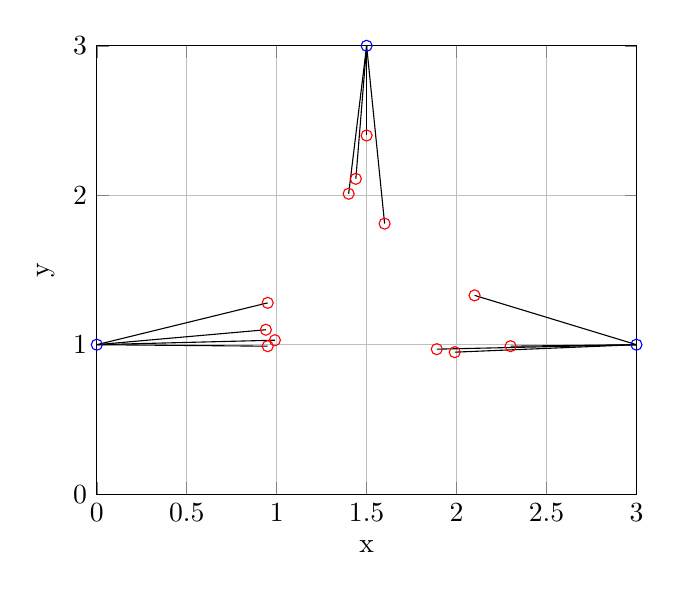
\begin{tikzpicture}
    \begin{axis}
    [
        xlabel={x}, 
        ylabel={y}, 
        grid, 
        xmin=0, 
        xmax=3, 
        ymin=0, 
        ymax=3, 
        tick align=inside
    ]
    \addplot[red, mark=o, only marks] coordinates {
        (0.94, 1.1)
        (0.95, 1.28)
        (0.95, 0.99)
        (0.99, 1.03)
        (1.89, 0.97)
        (1.99, 0.95)
        (2.1, 1.33)
        (2.3, 0.99)        
        (1.5, 2.4)
        (1.4, 2.01)
        (1.44, 2.11)
        (1.6, 1.81)
    };
    \addplot[blue, mark=o, only marks] coordinates {
        (0, 1)
        (1.5, 3)
        (3, 1)
    };
        \addplot[black] coordinates {(0,1) (0.94, 1.1)};
        \addplot[black] coordinates {(0,1) (0.95, 1.28)};
        \addplot[black] coordinates {(0,1) (0.95, 0.99)};
        \addplot[black] coordinates {(0,1) (0.99, 1.03)};
        \addplot[black] coordinates {(3, 1) (1.89, 0.97)};
        \addplot[black] coordinates {(3, 1) (1.99, 0.95)};
        \addplot[black] coordinates {(3, 1) (2.1, 1.33)};
        \addplot[black] coordinates {(3, 1) (2.3, 0.99)};      
        \addplot[black] coordinates {(1.5, 3) (1.5, 2.4)};
        \addplot[black] coordinates {(1.5, 3) (1.4, 2.01)};
        \addplot[black] coordinates {(1.5, 3) (1.44, 2.11)};
        \addplot[black] coordinates {(1.5, 3) (1.6, 1.81)};

    \end{axis}
\end{tikzpicture}
    \caption{Initial $\vmu$ and $\vpi$}
    \label{fig:9.1Ex1}
\end{figure}

\begin{figure}[h]
    \centering
    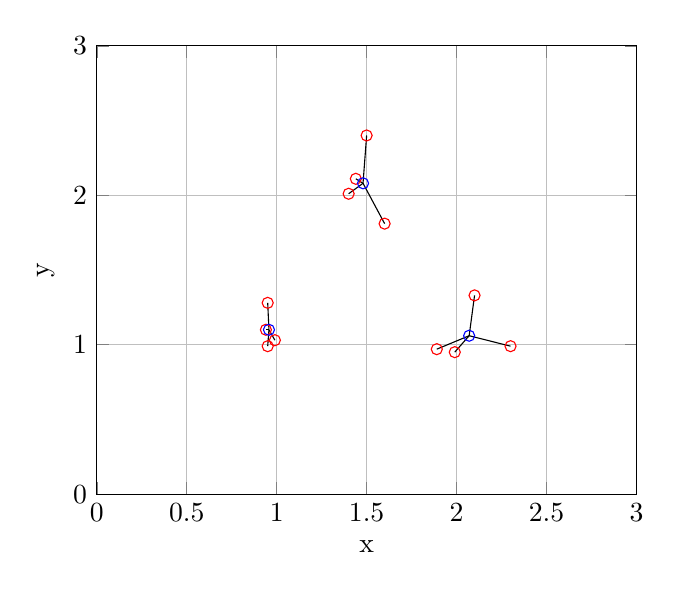
\begin{tikzpicture}
        \begin{axis}
        [
            xlabel={x}, 
            ylabel={y}, 
            grid, 
            xmin=0, 
            xmax=3, 
            ymin=0, 
            ymax=3, 
            tick align=inside
        ]
        \addplot[red, mark=o, only marks] coordinates {
            (0.94, 1.1)
            (0.95, 1.28)
            (0.95, 0.99)
            (0.99, 1.03)
            (1.89, 0.97)
            (1.99, 0.95)
            (2.1, 1.33)
            (2.3, 0.99)        
            (1.5, 2.4)
            (1.4, 2.01)
            (1.44, 2.11)
            (1.6, 1.81)
        };
        \addplot[blue, mark=o, only marks] coordinates {
            (0.957, 1.1)
            (2.07, 1.06)
            (1.48, 2.08)
        };
            \addplot[black] coordinates {(0.957, 1.1) (0.94, 1.1)};
            \addplot[black] coordinates {(0.957, 1.1) (0.95, 1.28)};
            \addplot[black] coordinates {(0.957, 1.1) (0.95, 0.99)};
            \addplot[black] coordinates {(0.957, 1.1) (0.99, 1.03)};
            \addplot[black] coordinates {(2.07, 1.06) (1.89, 0.97)};
            \addplot[black] coordinates {(2.07, 1.06) (1.99, 0.95)};
            \addplot[black] coordinates {(2.07, 1.06) (2.1, 1.33)};
            \addplot[black] coordinates {(2.07, 1.06) (2.3, 0.99)};      
            \addplot[black] coordinates {(1.48, 2.08) (1.5, 2.4)};
            \addplot[black] coordinates {(1.48, 2.08) (1.4, 2.01)};
            \addplot[black] coordinates {(1.48, 2.08) (1.44, 2.11)};
            \addplot[black] coordinates {(1.48, 2.08) (1.6, 1.81)};
    
        \end{axis}
    \end{tikzpicture}
    \caption{$\vmu$ and $\vpi$ after one iteration}
    \label{fig:9.1Ex2p}
\end{figure}

\end{example}

\begin{example}
Given a data set of matrices in $\R^{8\times 8}$ representing an $8$-by-$8$ black and white pixel image of handwritten digits, we would like to run $10$-means clustering, in hope that each digit is reasonably clustered (i.e. two digits are close if they are the same, and far apart if they are different.)

Then, after obtaining a value for $\vmu$, we can run predictions on unlabeled data to predict the digit that it corresponds to it with the center closest to it.
\end{example}

\section{Exercises}

\begin{enumerate}
    \item Suppose a streaming service uses cluster analysis to classify users in order to better tailor ads. Explain why this model would struggle to classify a shared account.
    \item Under what circumstances would a non-convex set would not be classifiable with $k$-means clustering?
    \item Although it was suggested that $M$ could be chosen arbitrarily, give an example where a bad initialization of $M$ would lead to the algorithm not producing reasonable clusters.
\end{enumerate}

\section{Solution To Exercises}
\begin{enumerate}
    \item A possible explanation might be that the metrics used are too irregular if there distinct users have sharp differences on their preferences.
    \item Non-convex sets are not captured precisely if distinct groups are too close, since $k$-means clusters data into spheres. However if the sets are far apart from each other, it is possible for the algorithm to classify data properly.
    \item If the set $M$ is initialized with very similar centers, then the algorithm might converge into overlapping spheres.
\end{enumerate}

\chapter{Feed Forward Neural Networks}

The goal of the following chapters is to introduce different types of neural network. To do so, we first introduce some definitions needed. 

\section{Abstract Neurons}\label{abstractneurons}

\begin{definition}
    An \define{abstract neuron}, or simply \define{neuron}, is a tuple $(\vx,\vw,\phi,y)$ where
    \begin{itemize}
        \item $\vx^\top = (x_0,\cdots,x_n)$ is the \define{input vector}, usually $x_0=-1$
        \item $\vw^\top = (w_0,\cdots,w_n)$ is the \define{weight vector}, with $w_0 = b$, the bias.
        \item $\phi:\R\to\R$ is the \define{activation function} of the neuron.
        \item $y=\phi(\vx^\top\vw)$ is the output of the neuron
    \end{itemize}
\end{definition}

The goal of the neuron is to take a target $z$, and "learn" the target by tunning $\vw$ such that $\phi(\vx^\top\vw) \approx z$ 

\begin{definition}
    A \define{perceptron} is a neuron with input $\vx\in\{0,1\}^n$ and activation function
    \begin{equation*}
        \phi(x) = 
        \begin{cases}
            1 & \text{if } x \geq 0\\
            0 & \text{if } x < 0
        \end{cases}
    \end{equation*}
    $\phi$ is called the \define{Heaviside} step function
\end{definition}

\begin{example}
    Let $f^*:\{0,1\}^2\to\{0,1\}$ be $f^*(x,y)=x\textbf{ and }y$. \\
    A solution using the Heaviside step function uses $\vw^\top = (1.5,1,1)$. Then $\vx^\top\vw = -1.5+x+y$, or equivalently, we have the line $y=1.5-x$
    \begin{figure}
    \centering
    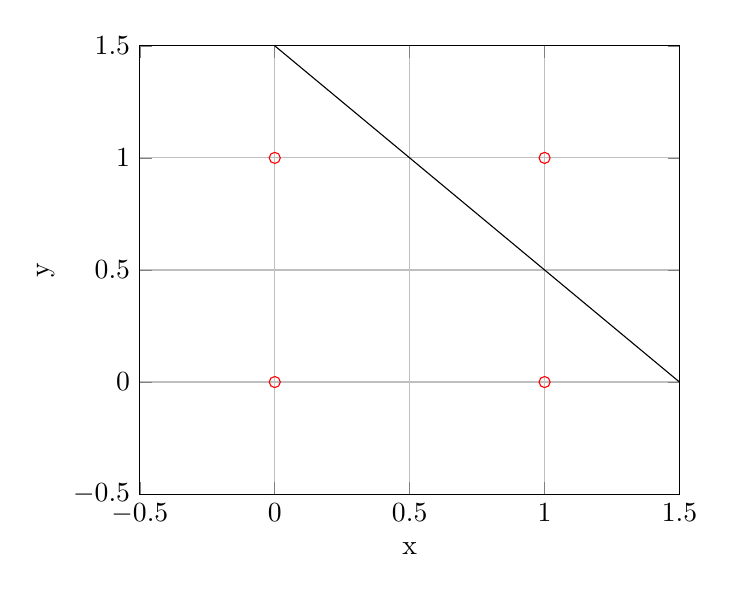
\begin{tikzpicture}
        \begin{axis}
        [
            xlabel={x}, 
            ylabel={y}, 
            grid, 
            xmin=-0.5, 
            xmax=1.5, 
            ymin=-0.5, 
            ymax=1.5, 
            tick align=inside
        ]
        \addplot[red, mark=o, only marks] coordinates {
            (0, 1)
            (0, 0)
            (1, 0)
            (1, 1)
        };
        \addplot[black] coordinates {(0, 1.5) (1.5, 0)};
        \end{axis}
    \end{tikzpicture}
    \caption{Outputs of \textbf{and} operator separated by $y=1.5-x$}
    \label{fig:9.1Ex2}
\end{figure}
\end{example}

\begin{example}
    Let $f^*:\{0,1\}^2\to\{0,1\}$ be $f^*(x,y)=x\textbf{ or }y$. \\
    A solution using the Heaviside step function uses $\vw^\top = (0.5,1,1)$. Then $\vx^\top\vw = -0.5+x+y$, or equivalently, we have the line $y=0.5-x$
    \begin{figure}
    \centering
    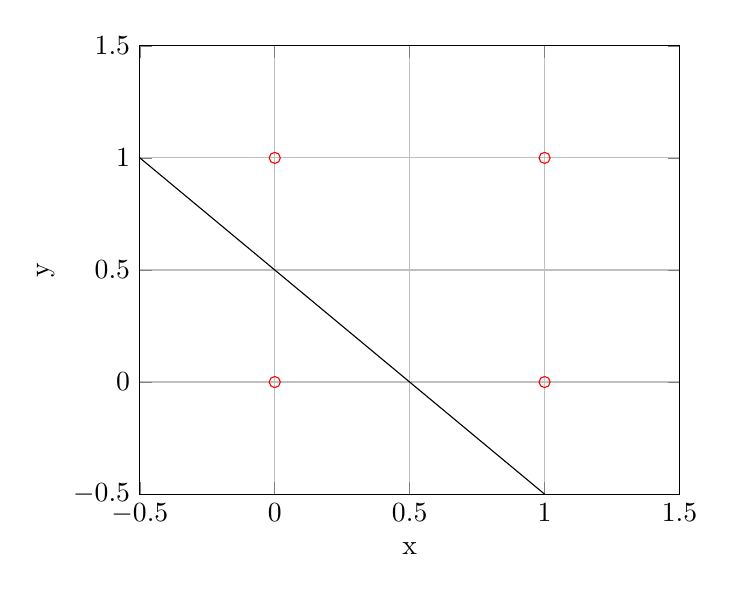
\begin{tikzpicture}
        \begin{axis}
        [
            xlabel={x}, 
            ylabel={y}, 
            grid, 
            xmin=-0.5, 
            xmax=1.5, 
            ymin=-0.5, 
            ymax=1.5, 
            tick align=inside
        ]
        \addplot[red, mark=o, only marks] coordinates {
            (0, 1)
            (0, 0)
            (1, 0)
            (1, 1)
        };
        \addplot[black] coordinates {(-0.5, 1) (1, -0.5)};
        \end{axis}
    \end{tikzpicture}
    \caption{Outputs of \textbf{or} operator separated by $y=0.5-x$}
    \label{fig:9.1Ex2}
\end{figure}
\end{example}

The examples above illustrate that if the points cannot be divided by a line (or hyperplane in higher dimensions) then we cannot learn the function using a single neuron. We will fix this later by using multiple neurons.

\section{The Sigmoid Neuron}

To better predicting the value of binary variable y, we need to make sure there is a strong gradient. So we can use sigmoid output.

\begin{definition}
    A neuron with sigmoid activation $\sigma$ \\
    $\sigma$($w^T$$\vx$) is usually interpreted as the probability that target z = 1.
\end{definition}

Given a supervised dataset X,$\Vec{\vy}$, for $y_i$ $\in$ {0,1} and $\forall$ i sampled from $P_{data}$($\Vec{x}$,$\vy$), we can try to learn target y via prediction.\\

\centerline {y = 1 if $\sigma$($w^T$$\vx$) > 0.5} 
\centerline {y = 0 if $\sigma$($w^T$$\vx$) < 0.5}

Linear Neurons: Neurons with activation $\varphi$(x) = x

\begin{definition}
    ReLU(rectified linear unit)\\
    Activation function
    \begin{equation*}
        ReLU(X) = xH(x) = \begin{cases}
        1 & \quad x < 0, \\
        0 & \quad x > 0.
        \end{cases}
    \end{equation*}
\end{definition}

\begin{center}
    \includegraphics[width=2.1in]{images/Chapter 10/ReLU.png}
\end{center}


\begin{example}
    A Network of Neurons: \\
    \centerline{$f(\Vec{x})=\Vec{x_1}$ x or $\Vec{x_2}$, for $\Vec{x}$ $\in$ $\{0,1\}^2$}\\
    
    \centerline{
       dataset X = $
       \begin{bmatrix}
        0 & 1\\
        1 & 0\\
        0 & 1\\
        1 & 1
    \end{bmatrix}
    $,
    $\Vec{y}$ = $ 
    \begin{bmatrix}
        0\\
        1\\
        1\\
        0
        \end{bmatrix}$}
we can draw points in X in the folowing figure


\begin{center}
    \includegraphics[width=3in]{images/Chapter 10/example1.png}
\end{center}




    Consider a modle f($\Vec{x}$,$\Vec{\theta}$) and cost function J($\theta$) = $\frac{1}{4}$ $\sum{(f^*(\Vec{x})-f(\Vec{x};\theta))}$

\begin{center}
    \includegraphics[width=3in]{images/Chapter 10/betterway.png}
\end{center}
    
    Idea: In $x_1$, $x_2$ - plane, the points are not separable by a line but maybe by transforing $x_1$, $x_2$ $\to$ $h_1$, $h_2$, the points can be separable by a line in the $h_1$, $h_2$ - plane.\\
    \centerline{
        $ \begin{pmatrix}
            h_{1}\\
            h_{2}
        \end{pmatrix} $ = ReLU($W^{(1)}\Vec{x}$ + $\vb^{(1)}$)
        }\\
    \centerline{
        Try $W^{(1)}$ = $ \begin{pmatrix}
            1 & 1\\
            1 & 1\\
        \end{pmatrix} $,
        $\Vec{\vb}^{(1)}$ = $ \begin{pmatrix}
            0\\
            -1
        \end{pmatrix} $
    }\\
    
    Apply to whole dataset.\\
    \begin{equation*}
         ReLU(XW^{(1)} + \Vec{1}\vb^{(1)}{}^T) = ReLU \left(
        \begin{pmatrix}
        0 & 0\\
        1 & 0\\
        0 & 1\\
        1 & 1
        \end{pmatrix} 
        \begin{pmatrix}
        1 & 1\\
        1 & 1
        \end{pmatrix} + 
        \begin{pmatrix}
        0 & -1\\
        0 & -1\\
        0 & -1\\
        0 & -1
        \end{pmatrix} \right)
    \end{equation*}
    \begin{equation*}  
        = ReLU \left(
        \begin{pmatrix}
        0 & 0\\
        1 & 1\\
        1 & 1\\
        2 & 2
        \end{pmatrix} 
        + \begin{pmatrix}
        0 & -1\\
        0 & -1\\
        0 & -1\\
        0 & -1
        \end{pmatrix} \right)
    \end{equation*}
    \begin{equation*}  
        = ReLU\begin{pmatrix}
        0 & -1\\
        1 & 0\\
        1 & 0\\
        2 & 1
        \end{pmatrix}\\
    \end{equation*}
    \begin{equation*}
        = \begin{pmatrix}
        0 & 0\\
        1 & 0\\
        1 & 0\\
        2 & 1
        \end{pmatrix}
    \end{equation*}


\begin{center}
    \includegraphics[width=4in]{images/Chapter 10/idea1.png}
\end{center}



So we can divide the point by y = $\frac{x}{2}$\\

Final output is
        $W^{(2)}$ $\begin{pmatrix}
        h_1\\
        h_2
        \end{pmatrix}$
        + $\vb^{(2)}$.
    Let $W^{(2)}$ = $\begin{pmatrix}
        1\\
        -2
        \end{pmatrix}$,
        $b^{(2)}$ = 0\\
        \begin{equation*}
            ReLU\left(
            \begin{pmatrix}
                0 & 0\\
                1 & 0\\
                1 & 0\\
                2 & 1
            \end{pmatrix}
            \begin{pmatrix}
                1\\
                -2
            \end{pmatrix}\right)
        \end{equation*}
        \begin{equation*}
            =ReLU
            \begin{pmatrix}
                0 \\
                1 \\
                1 \\
                0
            \end{pmatrix}
        \end{equation*}
        \begin{equation*}
            =\begin{pmatrix}
                0 \\
                1 \\
                1 \\
                0
            \end{pmatrix}
        \end{equation*}\\
        Better way to draw this:
    \begin{center}
        \includegraphics[width=3in]{images/Chapter 10/better.png}
    \end{center}
 \end{example}
 
 \begin{definition}
     A partially ordered set(poset) is a pair(P, $\leq$) where P is a set and $\leq$ is a relation on P s.t.\\
     1. x $\leq$ x, $\forall$ x $\in$ P\\
     2. if x $\leq$ y and y $\leq$ x then x = y $\forall$ x, y $\in$ P\\
     3.if x $leq$ y and y $\leq$ z then x $\leq$ z $\forall$ x, y, z $\in$ P
 \end{definition}

    Notation: Write x < y if x $\leq$ y and x $\neq$ y. Call (P, $\leq$) a total order if $\forall$ x, y $\in$ P x $\leq$ y or y $\leq$ x.\\
    
\begin{definition}
    A cover relation is a pair (x, y) s.t. x $\lneq$ y and $\nexists$ z with x < z < y.
\end{definition}

\begin{definition}
    The Hasse diagram of a finite poset (P, $\leq$) consists of a vertex for each x $\in$ P and a directed edge from x to y if and only if x $\in$ y draw from left to right. Write this as H(p).
\end{definition}

\begin{example}
    1.P = \{a, b, c, d\} a $\lneq$ b $\lneq$ c $\lneq$ d
    \begin{center}
        \includegraphics[width=2in]{images/Chapter 10/abcd.png}
    \end{center}
    2. P = \{S $\subseteq$ $\{1,2,3\}$ | S $\neq$ $\emptyset$ \} ordered by containment.
    \begin{center}
        \includegraphics[width=2in]{images/Chapter 10/P123.png}
    \end{center}
\end{example}

\begin{definition}
    A poset is graded if $\exists$ P: P $\rightarrow$ $\mathbb{N}$ (rank function) such that\\
    1. x < y $\implies$ $\rho$(x) < $\rho$(y), $\forall$ x, y $\in$ P\\
    2. x $\leftarrow$ y $\implies$ $\rho$(x) + 1 = $\rho$(y), $\forall$ x, y $\in$ P
\end{definition}

\begin{example}
    \{S $\subseteq$ {1,2,3} | S $\neq$ $\emptyset$ \} is graded \\
    i.e. in a graded poset there is a notiton of "depth"
\end{example}

Following is an example of not graded
\begin{center}
        \includegraphics[width=2in]{images/Chapter 10/nonbigraded.png}
\end{center}


The rank decomposition of a graded poset (P, $\leq$, $\rho$) is
\begin{equation*}
    P = \oplus Pi, Pi = \{ x \in P | \rho(x) = i \}
\end{equation*}

\begin{center}
    \includegraphics[width=2in]{images/Chapter 10/gradedp.png}
\end{center}

A linear extension of a poset (P, $\leq$) is a total ordering $\leq'$ on P s.t. x $\leq'$ y, for any x, y $\in$ P.\\
e.g\\.
\begin{center}
        \includegraphics[width=2in]{images/Chapter 10/linear.png}
\end{center}
b < a < c < d < e\\

\begin{lemma}
    A linear extension of a graded poset is determined by a choice of total ordering of each of its ranks. So there are $\prod_{i \in \mathbb{N}}$ |$P_{i}$|\\
\end{lemma}

Convention Drawing a Hasse diagram determines a linear extension by ordering downwards along ranks.\\
    \begin{center}
        \includegraphics[width=2in]{images/Chapter 10/convention.png}
    \end{center}
    a < b < c < d < e < f\\
So Hasse diagram contains all information.\\


\begin{definition}
    Let $N = (H,F,G)$ be a neural network with depth D and architecture $H$ = (P, $\leq$, $\rho$, $\leq'$).\\
    The feedforward of ${\vx} \in \mathbb{R}^{dim(V)_p^{D}}$ is:\\
        $N{\vx} = G_{D}F_{D-1}...G_{2}F_{1}G_{1}F_{0}{\vx} \in \mathbb{R}^{dim(V)_p^{D}}$
\end{definition}

\begin{example}
    $N$ = \\
     \includegraphics[width=2in]{images/Chapter 10/P123.png}\\
    \\
     Here in this example , ${\vb}^{0} = \begin{pmatrix}
        1\\
        1\\
        1\\
        \end{pmatrix}$ and ${\vb}^{1} = 0$.\\
    So our $N\begin{pmatrix}
        1\\
        1\\
        1\\
        \end{pmatrix} = G^{2}F^{1}G^{1}F^{0}\begin{pmatrix}
        1\\
        1\\
        1\\
        \end{pmatrix}$\\
        So:\\
        $F^{0}{\vx} = \begin{pmatrix}
        1 & -1 & 0\\
        2 & 0 & 3\\
        0 & -2 & -3\\
        \end{pmatrix}{\vx} + \begin{pmatrix}
        1\\
        1\\
        1\\
        \end{pmatrix}$\\
        and:\\
        $F^{1}{\vx} = \begin{pmatrix}
        1 & -2 & 1
        \end{pmatrix}$

    So now we get:\\
    $N\begin{pmatrix}
    1\\
    1\\
    1\\
    \end{pmatrix} = \sigma F^{1}ReLUF^{0} \begin{pmatrix}
        1\\
        1\\
        1\\
    \end{pmatrix} = \sigma F^{1}ReLU \begin{pmatrix}
    1\\
    6\\
    -4\\
    \end{pmatrix} = \sigma  F^{1} \begin{pmatrix}
    1\\
    6\\
    0\\
    \end{pmatrix} = \sigma(-1\phi) = \frac{1}{1+e^{11}}$ which is approximately = 0.0001.
           
        
\end{example}

\begin{example}
Suppose that $N$ has some depth D and $G^{1},...,G^{D}$ are all linear activations ($G^{i}{\vx} = {\vx}$ $\forall i$).\\
Then $N{\vx} = F^{D-1}F^{D-2}...F^{1}F^{0}{\vx}$.\\
    \begin{remark}\\
        The composition of affine maps is an affine map, so $\exists W, {\vb}$ such that\\
            $N{\vx} = W{\vx} + {\vb}$.\\
            (So this Neural network can only fit affine functions, in other words, this is essentially linear regression.)
    \end{remark}
\end{example}

\section{Neural Networks as Learning Algorithms}
Suppose there is a function $f^{*}:\mathbb{R}^{n} \mapsto \mathbb{R}^{k}$ (often k = 1) and we want to approximate or "model" $f^{*}$. Let $N$ be a neural network $N = (H,F,G)$ with depth D and $H = (P, \leq , \rho , \leq' )$ such that\\
 $\#P^{0} = n$ and $\#P^{D} = k$.\\
 \\
 Then we get $F^{i}{\vx} = W^{i}{\vx} + {\vb}^{i}$, where nonzero entries of $W^{i}$, and ${\vb}^{i}$ are treated as parameters.\\
 \\
 Let $W = (W^{0},...,W^{D-1})$ and $B = ({\vb}^{0},...,{\vb}^{D-1})$ and define $f_{model}({\vx};W,B) = N{\vx}$. (feedforward ${\vx}$).\\
 Now how do we find the appropriate values of W,B?\\
 Given a dataset $X \in \mathbb{R}^{mxn}$ and $Y \in \mathbb{R}^{mxk}$, we define a cost function:\\
\\
 $J(W,B) = \frac{1}{m} \sum_{i=1}^{m} L(f_{model}({\vx}^{i};W,B),{\vy}^{i})$.\\
and try to find values for W,B which minimize this cost function using some optimization algorithm.\\
\begin{note}
We will usually need to add a regularization term, which will be mentioned later in this chapter.\\
\\
A common choice for L is:\\
$L(f_{model}({\vx};W,B),{\vy}) = \norm{f_{model}({\vx};W,B) - {\vy}}_{2}^{2}$\\
\end{note}

\section{Neural Networks as a maximum likelihood estimator}
Lets assume X and Y are sampled from a distribution $p_{data}({\vx},{\vy})$ under I.I.D. assumptions.\\
Now let $p_{model}({\vy}|{\vx};\theta)$ be a model for $p_{data}({\vy}|{\vx})$, which has been parameterized by $\theta \in \mathbb{R}^{N}$ for some N.\\
Then $\theta_{ML} = \underset{\theta}{\mathrm{argmin}}(-\sum_{i=1}^{m}log(p_{model}({\vy}^{i}|{\vx}^{i};\theta))) $.\\
\\
\begin{example}
Suppose we choose $P_{model}$ to be Gaussian:\\
$P_{model}({\vy}|{\vx};W,B) =$ N$({\vy};N{\vx},\sum)$ where N is the normal distribution and $N$ is the neural network.\\
\\
Then $P_{model}({\vy}|{\vx};W,B) =$ N$({\vy};N{\vx},\sum)$ = $\frac{1}{\sqrt{2\pi^{n}det\sum}}exp(-\frac{1}{2}({\vy}-N{\vx})\sum^{-1}({\vy}-N{\vx}))$ where\\ $N = (H,F,G)$,\\ $F_{\vx}^{i} = W^{i}{\vx} + {\vb}^{i}$,\\ $W = (W^{0},...,W^{D-1})$, and\\ $B = ({\vb}^{0},...,{\vb}^{D-1})$.\\
\\
Then finding $\theta_{ML} = (W,B)_{ML}$ is equivalent to minimizing our cost function of the form:\\
$J(W,B) = -\sum_{i=1}^{m}log(\frac{1}{\sqrt{2\pi^{n}det\sum}}exp(-\frac{1}{2}({\vy}^{i}-N{\vx}^{i})\sum^{-1}({\vy}^{i}-N{\vx}^{0})))$\\
= $\frac{1}{m}\sum-log(\frac{1}{constant}+\frac{1}{2}({\vy}^{i}-N{\vx}^{i})\sum^{-1}({\vy}^{i}-N{\vx}^{i})$, which $\frac{1}{constant}$ does not affect argmin, so we can ignore this value.\\
Then:\\
$J(W,B) = \frac{1}{m}\sum_{i=1}^{m}\frac{1}{2}({\vy}^{i}-N{\vx}^{i})\sum^{-1}({\vy}^{i}-N{\vx}^{i})$.\\
    \begin{note}
        We can usually take $\sum = id$ by first normalizing the dataset if needed.
    \end{note}
which then we get:\\
$J(W,B) = \frac{1}{m}\sum_{i=1}^{m}\norm{{\vy}^{i}-N{\vx}^{i}}^{2}_{2}$.\\
\\
In the end, we cycle back to our previous cost function.\\
    \begin{note}
        So we can either specify a cost or specify a model for $p_{data}$ and can usually go back and forth between those.
    \end{note}
\end{example}
                     
     

\section{Exercises}
\begin{enumerate}
    \item Given X,${\vy}$, using sigmoid, ReLU, then sigmoid function to rectified linear unit.
       \begin{equation*}  
        X = \begin{pmatrix}
        2 & 1 & 1\\
        0 & 1 & 0\\
        0 & -3 & 2\\
        2 & -2 & 2
        \end{pmatrix},
        \vb^{(1)} = \begin{pmatrix}
         1\\
         0\\
         0\\
         1
        \end{pmatrix},
        \vb^{(2)} = \begin{pmatrix}
         1\\
         1\\
         1\\
         1
        \end{pmatrix},
        \vw^{(1)} =  \begin{pmatrix}
         0.5 & 1 & 2\\
         1 & 2 & 0.5\\
         2 & 0.5 & 1
        \end{pmatrix}
        \end{equation*}
        \begin{equation*}
         w^{(2)} =  \begin{pmatrix}
         1 & 2 & 0.5\\
         1 & 2 & 0.5\\
         1 & 2 & 0.5
        \end{pmatrix}
         \vw^{(3)} =  \begin{pmatrix}
         1\\
         0.5\\
         2
        \end{pmatrix},
        \vb^{(3)} = \begin{pmatrix}
         0\\
         1\\
         1\\
         0
        \end{pmatrix}
        \end{equation*}
    \item Draw a linear extension of poset (P, $\leq$), a < b < c < d < e < f
    \item Explain why we use sigmoid activation function to predict value of binary variable y.
    \item Determine the weight matrices $W^{(0)}, W^{(1)}, W^{(3)}, W^{(4)}$ for the following neural network if all connection weights are worth 1.
    
    \includegraphics[width=3in]{images/Chapter 10/Weights_Exercice.png}
    \item Find the output of the following neural network for 
    $\vx = \begin{pmatrix}
         1\\
         1\\
         1
        \end{pmatrix}$, 
    $\vb^{(0)} = \begin{pmatrix}
         1\\
         1\\
         1\\
         1
         \end{pmatrix}$
    $\vb^{(1)} = \begin{pmatrix}
         0\\
         \end{pmatrix}$


    \includegraphics[width=1.5in]{images/Chapter 10/NN_Exercice.png}
    
\end{enumerate}
\section{Solutions to Exercises}
\begin{enumerate}
    \item Start with plugging in the given data matrix in to the sigmoid equation: 
    \begin{equation*}
         sigmoid(XW^{(1)} + \Vec{1}\vb^{(1)}{}^T) = sigmoid \left(
        \begin{pmatrix}
        2 & 1 & 1\\
        0 & 1 & 0\\
        0 & -3 & 2\\
        2 & -2 & 2
        \end{pmatrix} 
        \begin{pmatrix}
         0.5 & 1 & 2\\
         1 & 2 & 0.5\\
         2 & 0.5 & 1
        \end{pmatrix} + 
        \begin{pmatrix}
        1 & 0 & 1\\
        1 & 0 & 1\\
        1 & 0 & 1\\
        1 & 0 & 1
        \end{pmatrix} \right)
    \end{equation*}
    \begin{equation*}
            =sigmoid
            \begin{pmatrix}
                5 & 4.5 & 6.5\\
                2 & 2 & 1.5\\
                2 & -5 & 1.5\\
                4 & -1 & 6
            \end{pmatrix}
            =
            \begin{pmatrix}
                0.73 & 0.99 & 1.00\\
                0.88 & 0.88 & 0.82\\
                0.88 & 0.01 & 0.82\\
                0.98 & 0.27 & 1.00
            \end{pmatrix}
        \end{equation*}
        \begin{equation*}
         ReLU(XW^{(2)} + \Vec{1}\vb^{(2)}{}^T) = ReLU \left(
        \begin{pmatrix}
                0.73 & 0.99 & 1.00\\
                0.88 & 0.88 & 0.82\\
                0.88 & 0.01 & 0.82\\
                0.98 & 0.27 & 1.00
        \end{pmatrix} 
        \begin{pmatrix}
         1 & 2 & 0.5\\
         1 & 2 & 0.5\\
         1 & 2 & 0.5
        \end{pmatrix} + 
        \begin{pmatrix}
        1 & 1 & 1\\
        1 & 1 & 1\\
        1 & 1 & 1\\
        1 & 1 & 1
        \end{pmatrix} \right)
    \end{equation*}
    \begin{equation*}
            =ReLU
            \begin{pmatrix}
                3.72 & 6.44 & 2.36\\
                3.58 & 6.16 & 2.29\\
                2.71 & 4.42 & 1.86\\
                3.25 & 5.5 & 2.13
            \end{pmatrix}
            =
            \begin{pmatrix}
                1 & 1 & 1\\
                1 & 1 & 1\\
                1 & 1 & 1\\
                1 & 1 & 1
            \end{pmatrix}
    \end{equation*}
    The final output is 
        $\begin{pmatrix}
        h_1\\
        h_2\\
        h_3\\
        h_4
        \end{pmatrix}$ $W^{(3)}$ 
    + $\vb^{(3)}$.
    \begin{equation*}
         sigmoid(XW^{(3)} + \Vec{1}\vb^{(3)}{}^T) = sigmoid \left(
        \begin{pmatrix}
                1 & 1 & 1\\
                1 & 1 & 1\\
                1 & 1 & 1\\
                1 & 1 & 1
        \end{pmatrix} 
        \begin{pmatrix}
         1\\
         0.5\\
         2
        \end{pmatrix} + 
        \begin{pmatrix}
        0\\
        1\\
        1\\
        0
        \end{pmatrix} \right)
    \end{equation*}
    \begin{equation*}
            =sigmoid
            \begin{pmatrix}
                3.5\\
                4.5\\
                4.5\\
                3.5
            \end{pmatrix}
            =
            \begin{pmatrix}
                0.97\\
                0.99\\
                0.99\\
                0.97
            \end{pmatrix}
    \end{equation*}
    \item The line extension of the given poset is:
        \begin{center}
            \includegraphics[width=2in]{images/Chapter 10/convention.png}
        \end{center}
    \item The reason why we choose to use sigmoid activation function is because the gradient is 0 when ${\vv^T}$h + ${\vb}$ outside the unit interval. Gradient equals to 0 means there's no direction to improve the parameter.
    \item
    $$
            W^{(0)} = \begin{pmatrix}
                1 & 1 & 0\\
                1 & 1 & 1\\
                1 & 1 & 1\\
                0 & 1 & 1
            \end{pmatrix},
            W^{(1)} = \begin{pmatrix}
                1 & 1 & 0 & 0\\
                1 & 1 & 1 & 1\\
                0 & 1 & 0 & 1\\
            \end{pmatrix},
            W^{(2)} = \begin{pmatrix}
                1 & 0 & 1\\
                1 & 1 & 1\\
                1 & 1 & 0\\
            \end{pmatrix},
            W^{(3)} = \begin{pmatrix}
                1 & 1 & 1\\
            \end{pmatrix}
 $$
\end{enumerate}

\section{Output Neural}
\begin{definition}
  Given a neural network  $N=(H, F, G)$  with depth  $D$ , for  $\vec{x} \in \mathbb{R}^{\# P_{0}} \cong V_{P}^{(0)}$  (an input vector), the hidden features associcted to  $\vec{x}$  at layer  $i$  are
$$
H F_{N}^{(i)} \vec{x}=G_{i} F_{i-1} \ldots F_{1} G_{1} F_{0} \vec{x}
$$
where  $ H F_{N}^{(0)} \vec{x}=\vec{x}$.  
\end{definition}


\begin{figure}[ht]
\centering
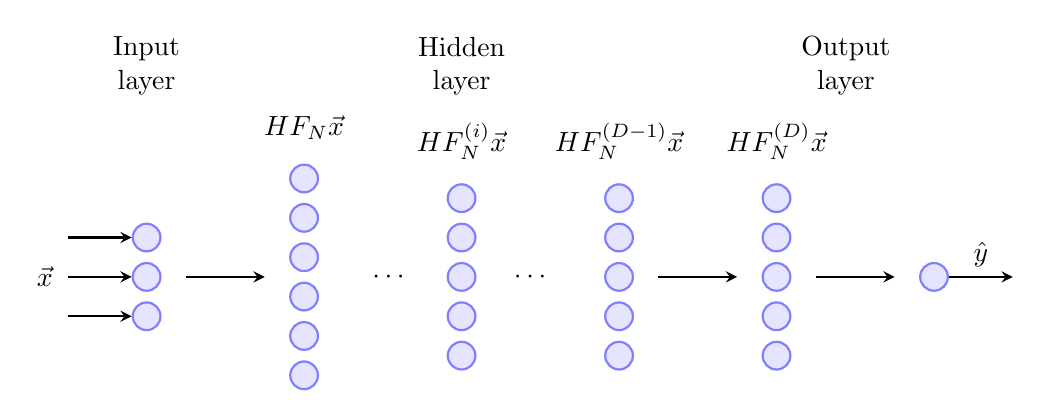
\begin{tikzpicture}
    \node[inputNode, thick] (i1) at (0, 0.5) {};
    \node[inputNode, thick] (i2) at (0, 0) {};
    \node[inputNode, thick] (i3) at (0, -0.5) {};
	
    \node[inputNode, thick] (h11) at (2, 1.25) {};
    \node[inputNode, thick] (h12) at (2, 0.75) {};
    \node[inputNode, thick] (h13) at (2, 0.25) {};
    \node[inputNode, thick] (h14) at (2, -0.25) {};
    \node[inputNode, thick] (h15) at (2, -0.75) {};
    \node[inputNode, thick] (h16) at (2, -1.25) {};

    
    \node[inputNode, thick] (h21) at (4, 1) {};
    \node[inputNode, thick] (h22) at (4, 0.5) {};
    \node[inputNode, thick] (h23) at (4, 0) {};
    \node[inputNode, thick] (h24) at (4, -0.5) {};
    \node[inputNode, thick] (h25) at (4, -1) {};

    \node[inputNode, thick] (h41) at (6, 1) {};
    \node[inputNode, thick] (h42) at (6, 0.5) {};
    \node[inputNode, thick] (h43) at (6, 0) {};
    \node[inputNode, thick] (h44) at (6, -0.5) {};
    \node[inputNode, thick] (h45) at (6, -1) {};

    \node[inputNode, thick] (h31) at (8, 1) {};
    \node[inputNode, thick] (h32) at (8, 0.5) {};
    \node[inputNode, thick] (h33) at (8, 0) {};
    \node[inputNode, thick] (h34) at (8, -0.5) {};
    \node[inputNode, thick] (h35) at (8, -1) {};
	\node[inputNode, thick] (o) at (10, 0) {};
    \node[left=1em of h23, align=center] (t12) {$\cdots$}; 
    \node[right=1em of h23, align=center] (t11) {$\cdots$}; 
    \node[left=2.5em of i2, align=center] (t2) {$\vec{x}$}; 
    \node[above=0.5em of h11, align=center] (t3) {$HF_N\vec x$};     
    \node[above=0.5em of h21, align=center] (t4) {$HF_N^{(i)}\vec x$};   
    \node[above=0.5em of h41, align=center] (t5) {$HF_N^{(D-1)}\vec x$};  
    \node[above=0.5em of h31, align=center] (t5) {$HF_N^{(D)}\vec x$};  
    \draw[stateTransition] (0.5,0) -- (1.5, 0);
    \draw[stateTransition] (6.5,0) -- (7.5, 0);
    \draw[stateTransition] (8.5,0) -- (9.5, 0);
    \draw[stateTransition] (-1, 0.5) -- (i1);
    \draw[stateTransition] (-1, 0)   -- (i2);
    \draw[stateTransition] (-1, -0.5)-- (i3);
    \draw[stateTransition] (o) -- node[above] {$\hat{y}$} (11, 0);
    \node[above=of h21, align=center] (l2) {Hidden \\ layer};
    \node[left=7.9em of l2, align=center] (l1) {Input \\ layer};
    \node[right=10em of l2, align=center] (l3) {Output \\ layer};
\end{tikzpicture}
\end{figure}
So the output neural are responsible for predicting the target from  $H F_{N}^{(D-1)} \vec{x}$ . The choice of activation at the output layer depends on the type of targets possible
(i.e. on  $  p_{\text {data }}(\vec{y})$)

 \begin{example}
     \begin{align*}
\text{Input: }&\vec{x}= \text{ (some statistics on two sports teams) }\\
&y=\left\{\begin{array}{ll}0 & \text { if } \operatorname{team} 1 \text { wins } \\ 1 & \text { if } \operatorname{team} 2 \text { wins }\end{array}\right.
\end{align*}

Dataset  $X, \vec{y}$  of previous result. Goal: predict winners of upcoming games.


Idea: Apply a neural network  $N$  so that
$$
N \vec{x}=p(y=1 \mid \vec{x})
$$

\begin{figure}[ht]
\centering
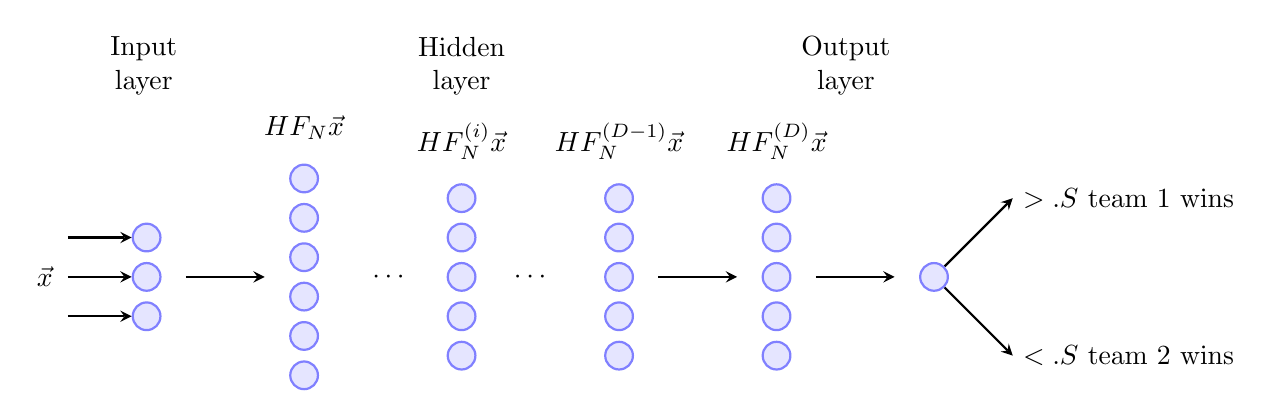
\begin{tikzpicture}
    \node[inputNode, thick] (i1) at (0, 0.5) {};
    \node[inputNode, thick] (i2) at (0, 0) {};
    \node[inputNode, thick] (i3) at (0, -0.5) {};
	
    \node[inputNode, thick] (h11) at (2, 1.25) {};
    \node[inputNode, thick] (h12) at (2, 0.75) {};
    \node[inputNode, thick] (h13) at (2, 0.25) {};
    \node[inputNode, thick] (h14) at (2, -0.25) {};
    \node[inputNode, thick] (h15) at (2, -0.75) {};
    \node[inputNode, thick] (h16) at (2, -1.25) {};

    
    \node[inputNode, thick] (h21) at (4, 1) {};
    \node[inputNode, thick] (h22) at (4, 0.5) {};
    \node[inputNode, thick] (h23) at (4, 0) {};
    \node[inputNode, thick] (h24) at (4, -0.5) {};
    \node[inputNode, thick] (h25) at (4, -1) {};

    \node[inputNode, thick] (h41) at (6, 1) {};
    \node[inputNode, thick] (h42) at (6, 0.5) {};
    \node[inputNode, thick] (h43) at (6, 0) {};
    \node[inputNode, thick] (h44) at (6, -0.5) {};
    \node[inputNode, thick] (h45) at (6, -1) {};

    \node[inputNode, thick] (h31) at (8, 1) {};
    \node[inputNode, thick] (h32) at (8, 0.5) {};
    \node[inputNode, thick] (h33) at (8, 0) {};
    \node[inputNode, thick] (h34) at (8, -0.5) {};
    \node[inputNode, thick] (h35) at (8, -1) {};
	\node[inputNode, thick] (o) at (10, 0) {};
    \node[left=1em of h23, align=center] (t12) {$\cdots$}; 
    \node[right=1em of h23, align=center] (t11) {$\cdots$}; 
    \node[left=2.5em of i2, align=center] (t2) {$\vec{x}$}; 
    \node[above=0.5em of h11, align=center] (t3) {$HF_N\vec x$};     
    \node[above=0.5em of h21, align=center] (t4) {$HF_N^{(i)}\vec x$};   
    \node[above=0.5em of h41, align=center] (t5) {$HF_N^{(D-1)}\vec x$};  
    \node[above=0.5em of h31, align=center] (t5) {$HF_N^{(D)}\vec x$};  
    \draw[stateTransition] (0.5,0) -- (1.5, 0);
    \draw[stateTransition] (6.5,0) -- (7.5, 0);
    \draw[stateTransition] (8.5,0) -- (9.5, 0);
    \draw[stateTransition] (-1, 0.5) -- (i1);
    \draw[stateTransition] (-1, 0)   -- (i2);
    \draw[stateTransition] (-1, -0.5)-- (i3);

    \draw[stateTransition] (o) -- (11, 1)  node[right] {$>.S$ team 1 wins};
    \draw[stateTransition] (o) -- (11, -1)  node[right] {$<.S$ team 2 wins};

    \node[above=of h21, align=center] (l2) {Hidden \\ layer};
    \node[left=8em of l2, align=center] (l1) {Input \\ layer};
    \node[right=10em of l2, align=center] (l3) {Output \\ layer};
\end{tikzpicture}
\end{figure}
Sigmoid activation makes sense here.
\end{example}

% \newpage
% \begin{figure}[ht]
% \centering
% \begin{tikzpicture}
%     \node[inputNode, thick] (i1) at (0, 0.5) {};
%     \node[inputNode, thick] (i2) at (0, 0) {};
%     \node[inputNode, thick] (i3) at (0, -0.5) {};
	
%     \node[inputNode, thick] (h11) at (2, 1.25) {};
%     \node[inputNode, thick] (h12) at (2, 0.75) {};
%     \node[inputNode, thick] (h13) at (2, 0.25) {};
%     \node[inputNode, thick] (h14) at (2, -0.25) {};
%     \node[inputNode, thick] (h15) at (2, -0.75) {};
%     \node[inputNode, thick] (h16) at (2, -1.25) {};

    
%     \node[inputNode, thick] (h21) at (4, 1) {};
%     \node[inputNode, thick] (h22) at (4, 0.5) {};
%     \node[inputNode, thick] (h23) at (4, 0) {};
%     \node[inputNode, thick] (h24) at (4, -0.5) {};
%     \node[inputNode, thick] (h25) at (4, -1) {};

%     \node[inputNode, thick] (h41) at (6, 1) {};
%     \node[inputNode, thick] (h42) at (6, 0.5) {};
%     \node[inputNode, thick] (h43) at (6, 0) {};
%     \node[inputNode, thick] (h44) at (6, -0.5) {};
%     \node[inputNode, thick] (h45) at (6, -1) {};

%     \node[inputNode, thick] (h31) at (8, 1) {};
%     \node[inputNode, thick] (h32) at (8, 0.5) {};
%     \node[inputNode, thick] (h33) at (8, 0) {};
%     \node[inputNode, thick] (h34) at (8, -0.5) {};
%     \node[inputNode, thick] (h35) at (8, -1) {};
% 	\node[inputNode, thick] (o) at (10, 0) {};
%     \node[left=1em of h23, align=center] (t12) {$\cdots$}; 
%     \node[right=1em of h23, align=center] (t11) {$\cdots$}; 
%     \node[left=2.5em of i2, align=center] (t2) {$\vec{x}$}; 
%     \node[above=0.5em of h11, align=center] (t3) {$HF_N\vec x$};     
%     \node[above=0.5em of h21, align=center] (t4) {$HF_N^{(i)}\vec x$};   
%     \node[above=0.5em of h41, align=center] (t5) {$HF_N^{(D-1)}\vec x$};  
%     \node[above=0.5em of h31, align=center] (t5) {$HF_N^{(D)}\vec x$};  
%     \draw[stateTransition] (0.5,0) -- (1.5, 0);
%     \draw[stateTransition] (6.5,0) -- (7.5, 0);
%     \draw[stateTransition] (8.5,0) -- (9.5, 0);
%     \draw[stateTransition] (-1, 0.5) -- (i1);
%     \draw[stateTransition] (-1, 0)   -- (i2);
%     \draw[stateTransition] (-1, -0.5)-- (i3);

%     \node[above=of h21, align=center] (l2) {Hidden \\ layer};
%     \node[left=8em of l2, align=center] (l1) {Input \\ layer};
%     \node[right=10em of l2, align=center] (l3) {Output \\ layer};
% \end{tikzpicture}
% \end{figure}
% $$
% \vec{x}^{(i)}=H F_{N}^{i}(\vec{x})=G^{(i)} F^{(i-1)} \ldots G^{(1)} F_{\Delta}^{(0)} \vec{x}
% $$

\begin{example}
 Input  $\vec{x}$  statstics on sports teams  1 \& 2 
$$
y=\left\{\begin{array}{rc}
1 & \text { team } 1 \text { wins } \\
0 & \text { team } 2 \text { wins }
\end{array}\right.
$$
Idea: want  $N \vec{x}=p(y=1 \mid \vec{x})$ 

\begin{figure}[ht]
\centering
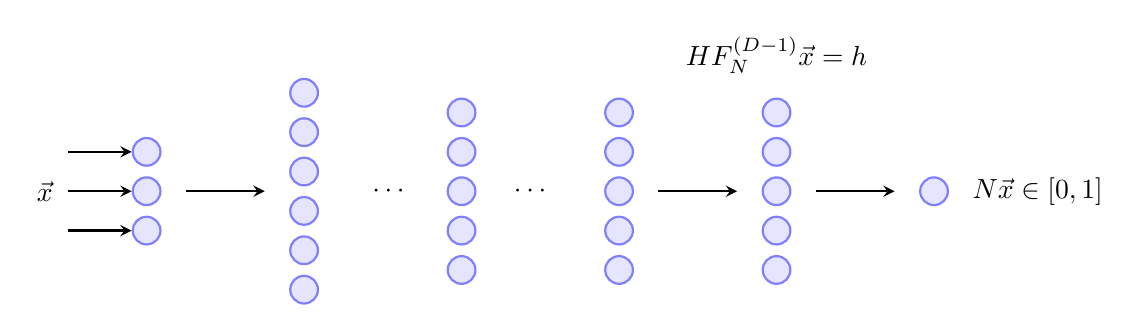
\begin{tikzpicture}
    \node[inputNode, thick] (i1) at (0, 0.5) {};
    \node[inputNode, thick] (i2) at (0, 0) {};
    \node[inputNode, thick] (i3) at (0, -0.5) {};
	
    \node[inputNode, thick] (h11) at (2, 1.25) {};
    \node[inputNode, thick] (h12) at (2, 0.75) {};
    \node[inputNode, thick] (h13) at (2, 0.25) {};
    \node[inputNode, thick] (h14) at (2, -0.25) {};
    \node[inputNode, thick] (h15) at (2, -0.75) {};
    \node[inputNode, thick] (h16) at (2, -1.25) {};

    
    \node[inputNode, thick] (h21) at (4, 1) {};
    \node[inputNode, thick] (h22) at (4, 0.5) {};
    \node[inputNode, thick] (h23) at (4, 0) {};
    \node[inputNode, thick] (h24) at (4, -0.5) {};
    \node[inputNode, thick] (h25) at (4, -1) {};

    \node[inputNode, thick] (h41) at (6, 1) {};
    \node[inputNode, thick] (h42) at (6, 0.5) {};
    \node[inputNode, thick] (h43) at (6, 0) {};
    \node[inputNode, thick] (h44) at (6, -0.5) {};
    \node[inputNode, thick] (h45) at (6, -1) {};

    \node[inputNode, thick] (h31) at (8, 1) {};
    \node[inputNode, thick] (h32) at (8, 0.5) {};
    \node[inputNode, thick] (h33) at (8, 0) {};
    \node[inputNode, thick] (h34) at (8, -0.5) {};
    \node[inputNode, thick] (h35) at (8, -1) {};
	\node[inputNode, thick] (o) at (10, 0) {};
    \node[left=1em of h23, align=center] (t12) {$\cdots$}; 
    \node[right=1em of h23, align=center] (t11) {$\cdots$}; 
    \node[left=2.5em of i2, align=center] (t2) {$\vec{x}$}; 
  
    \node[above=0.5em of h31, align=center] (t5) {$HF_N^{(D-1)}\vec x=h$};  
    \node[right=0.5em of o, align=center] (t6) {$N\vec x\in[0,1]$};
    \draw[stateTransition] (0.5,0) -- (1.5, 0);
    \draw[stateTransition] (6.5,0) -- (7.5, 0);
    \draw[stateTransition] (8.5,0) -- (9.5, 0);
    \draw[stateTransition] (-1, 0.5) -- (i1);
    \draw[stateTransition] (-1, 0)   -- (i2);
    \draw[stateTransition] (-1, -0.5)-- (i3);
\end{tikzpicture}
\end{figure}
Makes sense to use sigmoid activation for  $G^{(D)}$.
\end{example}
\begin{remark}
    This is equvalent  $p$  transforming  $\vec{x}$  to new features  $\vec{h}$  and performing logistic regression on  $\vec{h}$.
\end{remark}

\newpage

\begin{example}
    
$\vec{x}$  statistics about a company $y$ has stock price in 1 week ($y$ has continuous distribution e.g. Gaussian) 


linear activation  $G^{(D)}(y)=y$  makes sense here.

\begin{figure}[ht]
\centering
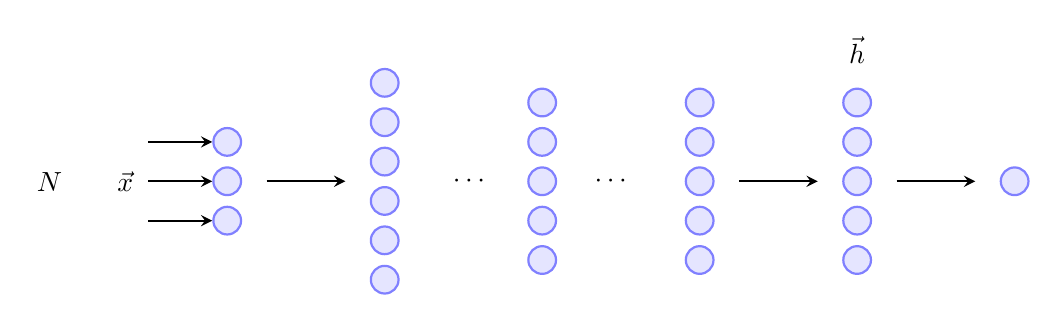
\begin{tikzpicture}
    \node[inputNode, thick] (i1) at (0, 0.5) {};
    \node[inputNode, thick] (i2) at (0, 0) {};
    \node[inputNode, thick] (i3) at (0, -0.5) {};
	
    \node[inputNode, thick] (h11) at (2, 1.25) {};
    \node[inputNode, thick] (h12) at (2, 0.75) {};
    \node[inputNode, thick] (h13) at (2, 0.25) {};
    \node[inputNode, thick] (h14) at (2, -0.25) {};
    \node[inputNode, thick] (h15) at (2, -0.75) {};
    \node[inputNode, thick] (h16) at (2, -1.25) {};

    \node[inputNode, thick] (h21) at (4, 1) {};
    \node[inputNode, thick] (h22) at (4, 0.5) {};
    \node[inputNode, thick] (h23) at (4, 0) {};
    \node[inputNode, thick] (h24) at (4, -0.5) {};
    \node[inputNode, thick] (h25) at (4, -1) {};

    \node[inputNode, thick] (h41) at (6, 1) {};
    \node[inputNode, thick] (h42) at (6, 0.5) {};
    \node[inputNode, thick] (h43) at (6, 0) {};
    \node[inputNode, thick] (h44) at (6, -0.5) {};
    \node[inputNode, thick] (h45) at (6, -1) {};

    \node[inputNode, thick] (h31) at (8, 1) {};
    \node[inputNode, thick] (h32) at (8, 0.5) {};
    \node[inputNode, thick] (h33) at (8, 0) {};
    \node[inputNode, thick] (h34) at (8, -0.5) {};
    \node[inputNode, thick] (h35) at (8, -1) {};
	\node[inputNode, thick] (o) at (10, 0) {};
    \node[left=1em of h23, align=center] (t12) {$\cdots$}; 
    \node[right=1em of h23, align=center] (t11) {$\cdots$}; 
    \node[left=2.5em of i2, align=center] (t2) {$N\qquad\vec{x}$}; 
  
    \node[above=0.5em of h31, align=center] (t5) {$\vec h$};  
    \draw[stateTransition] (0.5,0) -- (1.5, 0);
    \draw[stateTransition] (6.5,0) -- (7.5, 0);
    \draw[stateTransition] (8.5,0) -- (9.5, 0);
    \draw[stateTransition] (-1, 0.5) -- (i1);
    \draw[stateTransition] (-1, 0)   -- (i2);
    \draw[stateTransition] (-1, -0.5)-- (i3);
\end{tikzpicture}
\end{figure}
\end{example}

\begin{remark}
    This is equivalent to performing linear regression on  $HF_{N}^{(D-1)}(\vec{x})$
\end{remark}

\begin{example}
    $\vec{X}=$  vectorized image of an animals  $\left(\begin{array}{c}k \\ \text { types }\end{array}\right) $
$$
y=\left\{\begin{array}{ll}
e_{1} & \text { if cat } \\
e_{2} & \text { if dog } \\
\vdots & \\
e_{k} & \text { if llama }
\end{array}\right. \in \mathbb{R}^k = \langle e_1,e_2,\cdots,e_k \rangle
$$
(call a one hot encoding)
want $N \vec{x}=\hat{y} \text { where } \hat{y}_{i}=p\left(y=e_{i} \mid \vec{x}\right),  \left(\therefore\sum_{i=1}^{k} \hat{y}_{i}=1\right.$

\begin{figure}[ht]
\centering
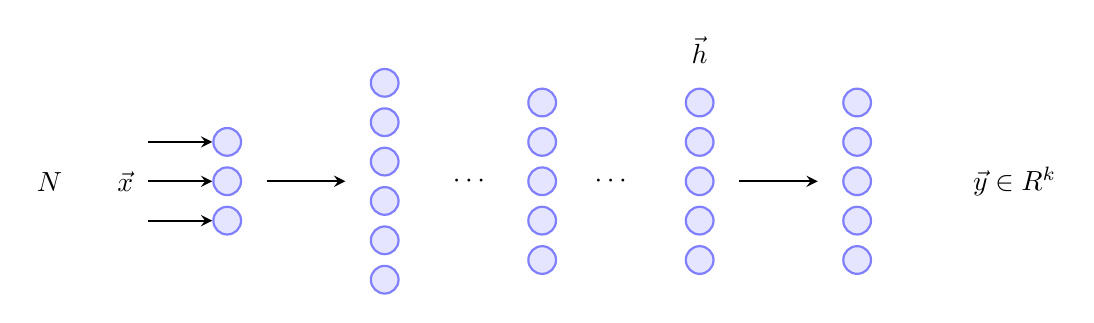
\begin{tikzpicture}
    \node[inputNode, thick] (i1) at (0, 0.5) {};
    \node[inputNode, thick] (i2) at (0, 0) {};
    \node[inputNode, thick] (i3) at (0, -0.5) {};
	
    \node[inputNode, thick] (h11) at (2, 1.25) {};
    \node[inputNode, thick] (h12) at (2, 0.75) {};
    \node[inputNode, thick] (h13) at (2, 0.25) {};
    \node[inputNode, thick] (h14) at (2, -0.25) {};
    \node[inputNode, thick] (h15) at (2, -0.75) {};
    \node[inputNode, thick] (h16) at (2, -1.25) {};

    \node[inputNode, thick] (h21) at (4, 1) {};
    \node[inputNode, thick] (h22) at (4, 0.5) {};
    \node[inputNode, thick] (h23) at (4, 0) {};
    \node[inputNode, thick] (h24) at (4, -0.5) {};
    \node[inputNode, thick] (h25) at (4, -1) {};

    \node[inputNode, thick] (h41) at (6, 1) {};
    \node[inputNode, thick] (h42) at (6, 0.5) {};
    \node[inputNode, thick] (h43) at (6, 0) {};
    \node[inputNode, thick] (h44) at (6, -0.5) {};
    \node[inputNode, thick] (h45) at (6, -1) {};

    \node[inputNode, thick] (h31) at (8, 1) {};
    \node[inputNode, thick] (h32) at (8, 0.5) {};
    \node[inputNode, thick] (h33) at (8, 0) {};
    \node[inputNode, thick] (h34) at (8, -0.5) {};
    \node[inputNode, thick] (h35) at (8, -1) {};
	\node (o) at (10, 0) {$\vec y \in \mathbb{R}^k$};
    \node[left=1em of h23, align=center] (t12) {$\cdots$}; 
    \node[right=1em of h23, align=center] (t11) {$\cdots$}; 
    \node[left=2.5em of i2, align=center] (t2) {$N\qquad\vec{x}$}; 
  
    \node[above=0.5em of h41, align=center] (t5) {$\vec h$};  
    \draw[stateTransition] (0.5,0) -- (1.5, 0);
    \draw[stateTransition] (6.5,0) -- (7.5, 0);
    \draw[stateTransition] (-1, 0.5) -- (i1);
    \draw[stateTransition] (-1, 0)   -- (i2);
    \draw[stateTransition] (-1, -0.5)-- (i3);
\end{tikzpicture}
\end{figure}

Define  $G^{(0)}=  \mathrm{softmax}$ where   $\mathrm{softmax}(\vec{h})=\frac{\exp _{p}\left(h_{i}\right)}{\sum_{j=1}^{k} \exp \left(h_{j}\right)}$ 
Softmax makes sense here.
\end{example}

\begin{remark}
    In each case we are choosing an activation function which will give the gradient nice properties. We want the gradient to have the property that when  $W, B$  are far from "local min, the gradient stays sufficiently large, (so GD does not "get stuck").
\end{remark}


\section{Optimization for Neural Networks}
Let  $N$  be a neural network and  $J(W, B)$  a cost function to measure "proximity" between  $N_{\vec{x}}$  and target  $\vec{y}$  on a dataset  $X, Y$ . To run gradient descent to find good values for $W,B$ we need to compute
$$
\frac{\partial J}{\partial W^{(i)}}, \frac{\partial J}{\partial b^{(i)}} \quad 0 \leq i \leq D-1
$$

Definition The signal ost of layer $i$ for input  $\vec{x}$  is
$$
S^{(i)}=F^{(i)} G^{(i)} \ldots G^{(1)} F^{(0)} \vec{x} \quad S^{(0)}=F^{(0)} \vec{x}
$$
\begin{remark}
    $G^{(i+1)} S^{(i)}=H F_{N}^{(i+1)}(\vec{x})=\vec{x}^{(i+1)}$ 
\end{remark}


\begin{example}

$$
\begin{array}{l}
W^{(0)}=\left(\begin{array}{ll}
w_{11}^{0} & w_{12}^{0} \\
w_{21}^{0} & w_{i 2}^{0}
\end{array}\right) \quad \vec{b}^{(0)}=\left(\begin{array}{l}
b_{i}^{i} \\
b_{2}^{0}
\end{array}\right) \\
W^{(1)}=\left(w_{11}^{\prime} w_{12}^{\prime}\right) \quad \vec{b}^{(1)}=\left(b_{1}^{\prime}\right) \\
S^{(0)}=W^{(0)} \vec{x}+\vec{b}^{(0)} \\
\vec{x}^{(1)}=G^{(1)}\left(s^{(0)}\right)=G^{(1)}\left(W^{(0)} \vec{x}+\vec{b}^{(0)}\right) \\
S^{(1)}=W^{(1)} G^{(1)}\left(S^{(0)}\right)+b^{(1)}=W^{(1)} \vec{x}^{(1)}+b^{(1)} \\
\vec{x}^{(2)}=G^{(2)}\left(s^{(1)}\right)=N \vec{x} \\
\end{array}
$$
    \begin{figure}[ht]
\centering
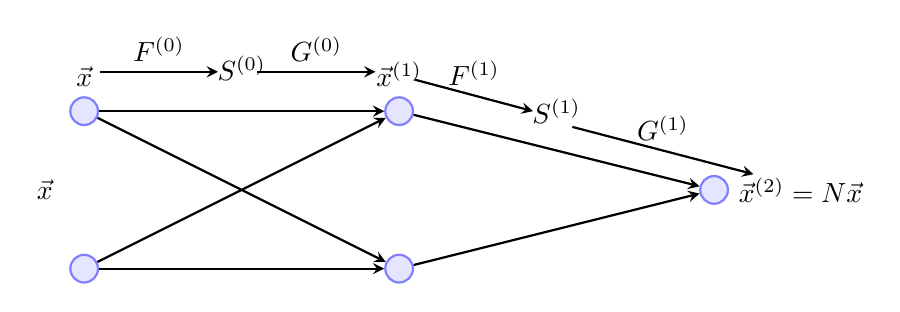
\begin{tikzpicture}
    \node[inputNode, thick] (i1) at (0, 1) {};
    \node[inputNode, thick] (i2) at (0, -1) {};
    \node[inputNode, thick] (h11) at (4, 1) {};
    \node[inputNode, thick] (h12) at (4, -1) {};
    \node[inputNode, thick] (o) at (8, 0) {};
    \node[align=center] (t1) at (-0.5,0) {$\vec{x}$}; 
  
    \draw[stateTransition] (i1) -- (h11);
    \draw[stateTransition] (i1) -- (h12);
    \draw[stateTransition] (i2) -- (h11);
    \draw[stateTransition] (i2) -- (h12);
    \draw[stateTransition] (h11) -- (o);
    \draw[stateTransition] (h12) -- (o);
    
    \node[ align=center] (t1) at (2,1.55) {$S^{(0)}$}; 
    \node[ align=center] (t2) at (6,1) {$S^{(1)}$};
    \node[above=0em of i1, align=center] (t3) {$\vec x$}; 
    \node[above=0em of h11, align=center] (t4) {$\vec x^{(1)}$}; 
    \node[right=0em of o, align=center] (t5) {$\vec x^{(2)}=N\vec x$};

    \draw[stateTransition] (0.2,1.5) -- node[above]{$F^{(0)}$} (1.7,1.5);
    \draw[stateTransition] (2.2,1.5) -- node[above]{$G^{(0)}$} (3.7,1.5);

    \draw[stateTransition] (4.2,1.4) -- node[above]{$F^{(1)}$} (5.7,1);
    \draw[stateTransition] (6.2,0.8) -- node[above]{$G^{(1)}$} (8.5,0.2);
\end{tikzpicture}
\end{figure}
Cost function  $J(W, B)=\sum_{i=1}^{m} L\left(N \vec{x}_{i}, \vec{y}_{i}\right) $. 
Need to find derivetives of  $L(N \vec{x}, \vec{y})$ 
\end{example}

\begin{remark}
    $\displaystyle\frac{\partial}{\partial v}(f \circ g)(v)=\left.\frac{\partial f(w)}{\partial w}\right|_{w=g(v)} \frac{\partial}{\partial v} g(v) $
$$
\text { where }\left.\frac{\partial f(w)}{\partial w}\right|_{w=g(v)}=\frac{\partial f}{\partial g(v)}
$$
\end{remark}

\section{Backpropagation}

Backpropagation is the algorithm we use to train feed forward neural networks. This algorithm efficiently computes the gradient of the loss function with respect to the weights of the network, adjusting the weights and biases of the model. This allows us to use gradient descent or stochastic gradient descent methods to train multilayer networks, updating weights to minimize loss.


We will explore backpropagation for a network defined by the poset $P(n_{0},n_{1},...n_{D})$, i.e., each layer is fully connected to adjacent layers, dataset $X\in\R^{m\times n}, Y\in\R^{m\times k}$ and a loss function
$$J(W,B)=\frac{1}{m}\sum_{i=1}^{m}L(N\vx_{i},\vy_{i})$$

\medskip
Now, let's find expressions for $\delta$, so we may use them to find expressions for the gradient of the loss function.
\begin{ceqn}
    \begin{align*}
        \delta^{(D-1)}&=\frac{\partial L}{\partial S^{(D-1)}}=\frac{\partial L}{\partial N\vx_{i}}\cdot\frac{\partial N\vx_{i}}{\partial S^{(D-1)}} \\
        &=\frac{\partial L}{\partial N\vx_{i}}\cdot\frac{\partial G^{(D)}}{\partial S^{(D-1)}}
    \end{align*}
\end{ceqn}
\begin{remark}
    Use $N\vx=G^{(D)}S^{(D-1)}$
\end{remark}
\smallskip
and for $0\leq l<D-1$:
\begin{ceqn}
\begin{align*}
    \delta^{(l)}&=\frac{\partial L}{\partial S^{(l)}}=\frac{\partial L}{\partial S^{(l+1)}}\cdot\frac{\partial S^{(l+1)}}{\partial S^{(l)}}\\
&=\delta^{(l+1)}W^{(l+1)}\frac{\partial G^{(l+1)}}{\partial S^{(l)}}
\end{align*}
\end{ceqn}
\begin{remark}
    Use $S^{(l+1)} = W^{(l+1)}G^{(l+1)}S^{(l+1)} + b^{(l+1)}$
\end{remark}
\medskip
With these handy values, we can now calculate:
\begin{ceqn}
\begin{align*}
    \frac{\partial L}{\partial W^{(l)}} &= \frac{\partial L}{\partial S^{(l)}}\cdot\frac{\partial S^{(l)}}{\partial W^{(l)}} \\
    &= \sum_{k=1}^{n_{l+1}}{\frac{\partial L}{\partial S_{k}^{(l)}}\cdot\frac{\partial S_{k}^{(l)}}{\partial W^{(l)}}} \\
    &= \sum_{k,j}{\delta_{k}^{(l)}\sum_{j=1}^{n_{l}}{\ME_{kj}\vx_{j}^{(l)}}} \\
    &= \sum_{k=1}^{n_{l+1}}{\delta_{k}^{(l)}\vx_{j}^{(l)}\ME_{kj}} \\
    &= \mathrm{outer}(\delta^{(l)},\vx^{(l)})
\end{align*}
\end{ceqn}

\begin{remark}
    Use $S_{k}^{(l)}=\sum_{j=1}^{n_l}{W_{k,j}^{(l)}x_j^{(l)}}+b_k^{(l)}$ \\
    Note that $\frac{\partial}{\partial W^{(l)}}W_{k,j}^{(l)}=\ME_{kj}$ where $\ME_{kj}$ is a matrix with an entry 1 in $(k,j)$ and zeros elsewhere.
\end{remark}

\smallskip
Similarly, we calculate:

\begin{ceqn}
\begin{align*}
    \frac{\partial L}{\partial b^{(l)}} &= \frac{\partial L}{\partial S^{(l)}}\cdot\frac{\partial S^{(l)}}{\partial b^{(l)}} \\
    &= \frac{\partial L}{\partial S^{(l)}} \\
    &= \delta^{(l)}
\end{align*}
\end{ceqn}

\medskip
Equipped with these partial derivatives with respect to the weight and bias matrices, we can now calculate the gradient for our arbitrary loss function:

$$J(W,B)=\frac{1}{m}\sum_{i=1}^{m}L(N\vx_{i},\vy_{i})$$

$$\frac{\partial J}{\partial W^{(l)}}=\frac{1}{m}\sum_{i=1}^{m}{\mathrm{outer}(\delta_{i}^{(l)},\vx_{i}^{(l)})}$$

$$\frac{\partial J}{\partial b^{(l)}}=\frac{1}{m}\sum_{i=1}^{m}\delta_{i}^{(l)}$$

\section{Regularization}

As we have learned with previous models, we do not want to train our feed forward neural network in such a way that the model is overfitted or underfitted. As such, we can use regularization to calibrate our model and minimize loss.

Let's consider stochastic gradient descent, a variant of gradient descent where only a few samples are selected randomly per iteration, instead of the complete data. We can take a look at the algorithm we use for each step:

\begin{algorithm}
    \caption{Regularization for Stochastic Gradient Descent Step}
    \begin{algorithmic}[1]
            \State Pick $\alpha > 0$
            \State Pick an arbitrary batch $Ba$
            \State Approximate $J(W,B)=\frac{1}{|Ba|}\sum_{i\in Ba}L(N\vx_{i},\vy_{i})$ and append to list of costs
		\For {$i \in Ba$}
        \State Compute [$(\vx_{i}^{(0)}, \S_{i}^{(0)}),\ldots,(\vx_{i}^{(D-1)}, \S_{i}^{(D-1)}),(\vx_{i}^{(D)})$]
        \State Compute [$\delta_{i}^{(D-1)},\ldots,\delta_{i}^{(0)}$]
        \State Compute $\frac{\partial J}{\partial W^{(l)}}=\frac{1}{|Ba|}\sum_{i\in Ba}{\mathrm{outer}(\delta_{i}^{(l)},\vx_{i}^{(l)})}$
		\State Compute $\frac{\partial J}{\partial b^{(l)}}=\frac{1}{|Ba|}\sum_{i \in Ba}\delta_{i}^{(l)}$
		\EndFor		
		\For {$l$ in range($D$)}
        \State $W^{(l)}= W^{(l)} - \alpha \frac{\partial J}{\partial W^{(l)}}$
        \State $b^{(l)}= b^{(l)} - \alpha \frac{\partial J}{\partial b^{(l)}}$
		\EndFor        
	\end{algorithmic} 
\end{algorithm}

If the correct neural network architecture is used, stochastic gradient descent can be used to find weights and biases that provide good performance on training and testing data.

\section{Common Loss Functions}

There are multiple loss (cost) functions we can use to train a feed forward neural network. Let's take a look at a few commonly used functions:

\smallskip
\begin{definition}
    \define{Square Error Loss} is defined by
    $$
    L_{SE}(N\vx,\vy) = ||N\vx-\vy||_{2}^{2}
    $$
\end{definition}
Square Error Loss is mostly used for linear regression, and is one of the simplest loss functions. The function ensures that the trained model has no outliers with huge errors, since a larger weight is assigned to such errors (thanks to the squaring part of the function).

\medskip
\begin{definition}
    \define{Cross Entropy Loss} is defined by
    \begin{ceqn}
    \begin{align*}
        L_{CE}(N\vx,\vy) &= -\vy^\top Log(N\vx) \\
        &= -\sum_{i=1}^{n_D}{\vy_i\log((N\vx)_i)}
    \end{align*}
    \end{ceqn}
\end{definition}
Cross Entropy Loss is used for multiclass classifiers which use softmax output neurons.

\medskip
\begin{definition}
    \define{Binary Cross Entropy Loss} is defined by
    $$
    L_{BCE}(N\vx,\vy) = -\vy^\top\log(N\vx) - (1-\vy)\log(1-N\vx)
    $$
\end{definition}
As its name suggests, Binary Cross Entropy Loss is used for binary classifiers, which use sigmoid output neurons.


\section{Vanishing Gradient Problem}
In practice, the function of a neural network N is non-convex, so there may be flat regions one may"get stuck" in during (stuck-stic) gradient descent.

\begin{center}
\includegraphics[width=4in]{images/Chapter 10/10.5(1).png}

\end{center}

\begin{remark}
Factors that affect the "flatness" of cost function:
\item 1. Choice of the loss function: $$
\begin{cases}
        SE & \text {lot of flat regions} \\
        CE & \text {less flat regions} \\
        BCE & \text {least of flat regions}
        \end{cases}
$$
2. Choice of activation(the ones we discussed so fare are good choices)

Note: Using several sigmoids in hidden layers can cause flatness.

Suggestion: Use ReLu in hidden layers

3. Momentum

4. Weight Initialization

\end{remark}


\subsection{Momentum Method}
Motivation(from physics). Momentum is one of the most popular techniques used to improve the speed of convergence of the Gradient Descent algorithm.

Consider a ball rolling on a surface

\begin{center}
\includegraphics[width=4in]{images/Chapter 10/10.5(2).png}

\end{center}

$$\text {f = potential function,  } {f\,({\vec{x})=m\,g\,x_3}}$$

$$\sum{\vec{F}\,=\,m\,\vec{a}\,\Longrightarrow\,\ddot{\vec{x}}}\,=\,\rho\,\dot{\vec{x}}\,-\,\nabla{f}(\vec{x})$$


To solve: Express as a system of First order ODEs
$$
\dot{\vec{V}}\,=\,-\rho\,\vec{v}\,-\,\nabla{f}(\vec{x})$$
$$\dot{\vec{x}}\,=\,\vec{V}$$

Write this as a finite difference system
(Pick $\nabla{t}$ small enough so that $\rho\,\nabla{t}\,<\,1$)
$$
\vec{V}_{n+1}\,-\,\vec{V}_n\,=-\rho\,\vec{V}_n\,\nabla{t}\,-\,\nabla{f(\vec{x}_n)}\,\nabla{t}
$$
$$
\vec{X}_{n+1}\,-\,\vec{X}_n\,=\,\vec{V}_{n+1}\,\nabla{t}
$$

Let $\epsilon\,=\,\nabla{t}\,$,$\,\,\mu\,=1-\rho\,\epsilon\,$ with$\,\,\,0\leq\mu\,<\,1$
$$
\vec{V}_{n+1}\,=\,\mu\,\vec{V}_n\,-\,\epsilon\,\nabla{f(\vec{x}_n)}
$$
$$
\vec{X}_{n+1}\,=\,\vec{X}_n\,+\,\epsilon\,\vec{V}_{n+1}
$$

let $\vec{V}\,\epsilon\,=\Tilde{\vec{V}}\,\,\,\text{(new scale for velocity)}$
$$
\frac{\tilde{\vec{V}}_{n+1}}{\epsilon}\,=\frac{\mu\,\tilde{\vec{V}}_{n}}{\epsilon}\,-\,\epsilon\,\nabla{f(\vec{x}\,n)}
$$

Define $\alpha\,=\,\epsilon^2$
$$
\tilde{\vec{V}}_{n+1}\,=\,\mu\,\tilde{\vec{V}}_n\,-\,\alpha\,\nabla{f(\vec{x}\,n)}$$
$$
\vec{X}_{n+1}\,=\,\vec{X}_n\,+\,\tilde{\vec{V}}_{n+1}$$

if $\mu=0$, this is just a gradient descent

\begin{example}
The problem with gradient descent is that the weight update at a moment (t) is governed by the learning rate and gradient at that moment only. It doesn’t take into account the past steps taken while traversing the cost space.
$$\nabla{w(t)}\,=\,-\eta\delta(t)$$
The gradient of the cost function at saddle points( plateau) is negligible or zero, which in turn leads to small or no weight updates. Hence, the network becomes stagnant, and learning stops.
(a) How can momentum fix this?


Solution: Imagine you have a ball rolling from point A. The ball starts rolling down slowly and gathers some momentum across the slope AB. When the ball reaches point B, it has accumulated enough momentum to push itself across the plateau region B and finally follow slope BC to land at the global minima C.

(b) How can this be used and applied to Gradient Descent?


Solution: To account for the momentum, we can use a moving average over the past gradients. In regions where the gradient is high like AB, weight updates will be large. Thus, in a way we are gathering momentum by taking a moving average over these gradients. But there is a problem with this method, it considers all the gradients over iterations with equal weight-age. The gradient at t=0 has equal weight-age as that of the gradient at the current iteration t. We need to use some sort of weighted average of the past gradients such that the recent gradients are given more weight-age.

\end{example}



\subsection{Weight Initialization}
Weight initialization is an important consideration in the design of a neural network model.

~\\Neural network models are fit using an optimization algorithm called stochastic gradient descent that incrementally changes the network weights to minimize a loss function, hopefully resulting in a set of weights for the mode that is capable of making useful predictions.

~\\The nodes in neural networks are composed of parameters referred to as weights used to calculate a weighted sum of the inputs.
Neural net performance depends heavily an $W^{(l)}$ weight initialization \underline{especially} if D is large. Depends less on bias initialization $b^{(l)}$ but this depends on architecture.

~\\\textbf{Claim}: 
\textcircled{1} If the initialized values of $W^{(l)}$ are too small, the variance of $J^{(l)}$ decreases at each layer 
\textcircled{2} If initialized weights are too large, variance $s^{(l)}$ amplifies at each layer.


\subsection{Xavier Initialization} Based on the assumption that Var($s^{(\lambda)}$ should remain constant at each layer.

For P($n_{0}$,...,$n_{0}$) entries of $W^{(l)}$ should be sampled from $N(x;0,\frac{2}{n_{l-1}+n_{l}})$.

~\\Many other "suggestions" exist

- Read section 8.4 of the Deep Learning book

- Read section 6.3 of the Deep Learning Architectures

Bias can usually be initialized to $\vec{O}$ \par


~\\\underline{A way to do SGD on neural net N} (for P($n_{0},...,n_{0}$))\\

Pick $\alpha_{step size}$\textless{0}, $\lambda_{reg-parameter}$\textless{0}, $\mu_{momentum}$\textless{0}, max\_iters, batch\_size


For $0\leq {l} \leq D-1$ initialize $W^{(l)}$ by sampling $N(x;0,\frac{2}{n_{l-1}+n_{l}})$
$b^{(o)} = \vec{(O)}$

\hspace{3cm}{initialize $V_{w}^{(l)} = np.zeros(W^{(l)}.shape)$

\hspace{3cm}$V_{b}^{(l)} = np.zeros(b^{(l)}.shape)$}

$epochs = 0$\\

While epochs \textless{max\_iters}:

\hspace{0.5cm}randomly pick $B\subseteq \{1,...,m\} with \|B\| = batch\_size$

\hspace{0.5cm}for $i \in B$:

\hspace{1cm}compute $[(x_{i}^{(0)},s_{i}^{(0)},(x_{i}^{(1)},s_{i}^{(1)}),...,(x_{i}^{(D-1)},s_{i}^{(D-1)}),(x_{i}^{(0)})]$

\hspace{1cm}compute $\delta_{i}^{(D-1)}$,...,$\delta_{i}^{(0)}$

\hspace{0.5cm}compute $\frac{\partial{J}}{\partial{W}^{(l)}}$

\hspace{0.5cm}for $0\leq l \leq D-1$:

\hspace{1cm} $V_{w}^{(l)}$ =$ \mu V_{w}^{(l)}-\alpha \frac{\partial{J}}{\partial{W}^{(l)}}$

\hspace{1cm} $V_{b}^{(l)}$ =$ \mu V_{b}^{(l)}-\alpha \frac{\partial{J}}{\partial{b}^{(l)}}$

\hspace{1cm} $W^{(l)} = W^{(l)} + V_{W}^{(l)}$

\hspace{1cm} $b^{(l)} = b^{(l)} + V_{b}^{(l)}$

\hspace{0.5cm}append cost to list of costs

return W, B, costs

\begin{example}
Derive Xavier Initialization
$$W_{i,j}^{[l]}\,=\,N(0,\,\frac{1}{n^{[l-1]}}$$

Solution:
\begin{center}
\includegraphics[width=4in]{images/Chapter 10/10.5(3).png}

\end{center}

\end{example}

\begin{example}
How is a$ W_{i}$ calculated when using Xavier initialization?
For a current Layer, let s be the output connections of the layer and e the input connections, then: $ f(W)= \frac{2}{e+s} $

~\\Solution:

In the case of Xavier initialization (also called "Glorot normal" in some software), the parameters are initialized as random draws from a truncated normal distribution with mean 0 and standard deviation

$\sigma = \sqrt{\frac{2}{a+b}}$

where a is the number of input units in the weight tensor, and b is the number of output units in the weight tensor.
\end{example}

\section{Exercises}
\begin{enumerate}
    \item Given $N\vx=[1.0, 0.8, 0.2]$ and $\vy=[1, 1, 0]$, compute the per-example loss for the following functions:
    \begin{enumerate}
        \item Square Error Loss $L_{SE}(N\vx, \vy)$
        \item Cross Entropy Loss $L_{CE}(N\vx, \vy)$
    \end{enumerate}
    \item Given $N\vx=[0.7]$ and $\vy=[1]$, find the Binary Cross Entropy Loss $L_{BCE}(N\vx, \vy)$
    \item How does squared error affect backpropagation? Derive an expression for $\delta^{(D-1)}$ where $L=L_{SE}$
\end{enumerate}

\subsection{Solutions}
\begin{enumerate}
    \item The per-example loss for the functions is:
    \begin{enumerate}
        \item $L_{SE}(N\vx, \vy) = 0.08$
        \item $L_{CE}(N\vx, \vy) = 0.2231435513142097$
    \end{enumerate}
    \item $L_{BCE}(N\vx, \vy) = 0.10536051565782628$
    \item First, let us compute the gradient of the loss function with respect to $N\vx$:
    \begin{align*}
        L_{SE}(N\vx,\vy) &= ||N\vx-\vy||_{2}^{2} \\
        \frac{\partial L_{SE}}{\partial N\vx} &= 2(N\vx-\vy)^\top
    \end{align*}
    Then, we can substitute to get
    \begin{align*}
        \delta^{(D-1)} &= \frac{\partial L_{SE}}{\partial N\vx}\cdot\frac{\partial N\vx}{\partial S^{D-1}} \\
        &= 2(N\vx-\vy)^\top\cdot\frac{\partial N\vx}{\partial S^{D-1}}
    \end{align*}
\end{enumerate}

\chapter{Convolutional Neural Networks}

\section{Introduction}

\subsection{Idea} In order to introduce convolutional neural networks, let's explore the role they play in neural networks.
A neural network architecture should be chosen in accordance to the type of structure of input data. Consider the following example.

\begin{example}
A data matrix X containing data such as statistics on houses with no real structure may use a fully connected architecture. Instead, let's take the example where X is a matrix with rows  of image pixel data. \\\\ Take this image to be a black and white image thay may be represented by a 3x3 matrix of pixels where each pixel is a level of "darkness" defined by the values: 0,1,2,3.\\

\includegraphics[scale=0.40]{images/Chapter 11/pic1.png}
\quad
\\
Pixels may be placed in a row by arranging the columns in order of their index as features.\\\\
\includegraphics[scale=0.40]{images/Chapter 11/pic2.png}
\\\\
We get the vector $(x_1,x_2,x_3,x_4,x_5,x_6,x_7,x_8,x_9)$.
Note that in the 3x3 matrix, $x_4$ is near $x_1$ and $x_7$, but the vector looses this structure. \\\\
This is our motivation for introducing a new type of layer to our neural network called a convolutional layer, in order to preserve a particular "structure" of the image. 

\end{example}


\section{Convolutional Layers}
\subsection{Convolutional Layer with 1D Inputs}
%---------------definition----------------------------------------------------------
\begin{definition}
%undefined control sequence?
    A discrete 1-D signal is a sequence $y=(y_i)_{i\in\mathbb{Z}}$ of real numbers and is $L^1$-finite if $\sum|y_k| < \infty$ and compact if there exists N such that $|k| >$ N $\Rightarrow y_k=0$.
    A 1-D kernel is a compact support signal of weights, w. Where $w = (w_i)_{i\in\mathbb{Z}}$. Since usually we want w to be a probability distribution, then $\Sigma_{i}w_i = 1$.
\end{definition}
%----------------------------------------------------------------------------------
%undefined control sequence?
Thus, the convolution, often called the cross correlation in signal processing, of y and w is $z=y*w$ where $z_{j} = \sum_{k\in\mathbb{Z}} y_{y+k}w_{k}$
%---------------example 2----------------------------------------------------------
\begin{example} \quad
\\
let
$w_i = \begin{cases}
    1/2 &\text{if} \quad i=0,1\\
    0 &\text{else}
\end{cases}$
\\
So $(y+w)_i=\sum_{k\in\mathbb{Z}} y_{i+k}w_k=\frac{y_i+y_{i+1}}{2}$
\end{example}
%-----------------------------------------------------------------------------------
\noindent
\\
More generally,
$w_i = \begin{cases}
    1/M &\text{if} \quad i=0,...,M-1\\
    0 &\text{else}
\end{cases}$
\\
%undefined control sequence?
Now $(y+w)_i=\sum_{k\in\mathbb{Z}} y_{i+k}w_k=\frac{y_i+y_{i+1}+...+y_{i+M-1}}{M}$
\\
\begin{example} \quad
\\
let $y=(1,2,3,4,5,6)$ and $w=(\frac{1}{2},\frac{1}{2})$
\\
Here $y+w = (\frac{1}{2},\frac{3}{2},\frac{5}{2},\frac{7}{2},\frac{9}{2},\frac{11}{2},3)=\frac{y_i+y_{i+1}}{2}$
\\
The operation is as follows
\\\\
$\begin{pmatrix}
\frac{1}{2}&\frac{1}{2} & & & & & &\\
& \frac{1}{2}&\frac{1}{2} & & & \text{\huge0}& &\\
&& \frac{1}{2}&\frac{1}{2} & & & &\\
&&& \frac{1}{2}& \frac{1}{2} & & &\\
&&&&\frac{1}{2} &\frac{1}{2} & &\\
&&\text{\huge0}&&&\frac{1}{2} &\frac{1}{2} &\\
&&&&&&\frac{1}{2} &\frac{1}{2}
\end{pmatrix}$
$\begin{pmatrix}
1\\2\\3\\4\\5\\6
\end{pmatrix}$
=
$\begin{pmatrix}

\frac{1}{2}(0) + \frac{1}{2}(1)\\
\frac{1}{2}(1) + \frac{1}{2}(2)\\
\frac{1}{2}(2) + \frac{1}{2}(3)\\
\frac{1}{2}(3) + \frac{1}{2}(4)\\
\frac{1}{2}(4) + \frac{1}{2}(5)\\
\frac{1}{2}(5) + \frac{1}{2}(6)\\
\frac{1}{2}(6) + \frac{1}{2}(7)\\
\end{pmatrix}
$
=
$
\begin{pmatrix}
\frac{1}{2}\\
\frac{3}{2}\\
\frac{5}{2}\\
\frac{7}{2}\\
\frac{9}{2}\\
\frac{11}{2}\\
3\\
\end{pmatrix}
$
\end{example}
\quad
\\
\noindent
When we use this in a neural network layer, we usually ignore the first and last component. We may also ignore some parts on the inside or only use alternating entries.

\subsection{Convolutional Layer with 3D Inputs}
\begin{example}\label{ex:CNNanimal}
In this example, we look at a neural network which uses two convolutional layers that takes images of animals and outputs a prediction of cat, dog, bear or pig.

\begin{figure}[H]
    \centering
    \includegraphics[scale=0.35]{images/Chapter 11/convolutionalNNexample.png}
    \caption{Neural network using convolutional layers to predict images of cat, dog, bear and pig.}
    \label{fig:11.1}
\end{figure}
The input consists of images of animals stored as $H\times K$ dimensions with $3$ color channels containing its associated RGB data. As discussed in the previous section, every signal passing through a convolutional layer will increase the number of features multiplicatively. This can be see in the formula to compute the $l$-th signal $Z^{(l)}$ given kernel $W^{(l)}$, bias $b^{(l)}$ and previous signal $Z^{(l-1)}$ which has $f_in$ features:
$$Z_{i,j,c,(f_{\text{in}},f_{\text{out}})}^{(l)} = G \left[ \left( \sum_{s,p}Z^{(l)}_{i+p,j+s,c,f_{\text{in}}} W_{p,s,c,(f_{\text{in}},f_{\text{out}})}^{(l)} \right) + b^{(l)}_{i,j,c,(f_{\text{in}},f_{\text{out}})}\right].$$

\noindent In this case, and in general, we find that
\begin{ceqn}
    \begin{align*}
        H^{(2)} &\leq H^{(1)} \leq H\\
        K^{(2)} &\leq K^{(1)} \leq K\\
        f^{(1)}f^{(2)} &\geq f^{(1)} \geq 1
    \end{align*}
\end{ceqn}
$H^{(l)}$ and $K^{(l)}$ is nonincreasing since we are applying convolution (see [relevant section when it gets written]). Sometimes, we want to preserve the size of $H^{(l)}$ and $K^{(l)}$ in all layers of our network. Moreover, the number of nodes $N$ in the example can be very large and computationally costly. To mitigate this problem, we introduce a padding and pooling process into our neural network.\\
\end{example}
\subsection{Padding}
\begin{definition}\label{def:Def11.1.1}
    For any matrix $\textbf{A} \in \mathbb{R}^{m,n}$, a \define{$p-$padding} applied to $\textbf{A}$ is the transformation $\textbf{I}_L\textbf{A}\textbf{I}_R$, where $\textbf{I}_L \in \mathbb{R}^{m+2p\times m}$ and $\textbf{I}_R \in \mathbb{R}^{n \times n+2p}$ such that
    $$(\textbf{I}_L)_{i,j} = \begin{cases} 1 & \text{ if } i = j-1 \text{ and } p+1 \leq i \leq m + 2p - 1\\ 
    0 & \text{ else } \end{cases}$$
    and
    $$(\textbf{I}_R)_{i,j} = \begin{cases} 1 & \text{ if } j = i+1 \text{ and }  p+1\leq j \leq n+2p-1\\ 
    0 & \text{ else } \end{cases}$$
\end{definition}
In simpler terms, if we have a matrix $\textbf{A} = \begin{bmatrix} a_{1,2} & a_{2,2} \\ a_{2,1} & a_{2,2} \end{bmatrix}$ and we apply $1-$padding to this, we will obtain a result of the form
$$\textbf{A}_{\text{padded}} =
\begin{bmatrix}
0 & 0 & 0 & 0 \\
0 & a_{1,1} & a_{1,2} & 0 \\
0 & a_{2,1} & a_{2,2} & 0 \\
0 & 0 & 0 & 0
\end{bmatrix}
$$
That is, we ``surround" the entries of $\textbf{A}$ with zeros.\\

\noindent Now suppose we have a $4 \times 4$ image, and we perform a convolution with stride $1$ and kernel of size $(2 \times 2)$. Then
$$
(4 \times 4) \ast_{(1,1)} (2 \times 2) = (3 \times 3)
$$
% To apply a 1-padding, we ``surround" our $(4 \times 4)$ input matrix with zeros, i.e.

% \begin{ceqn}
%     \begin{align*}
%     H = 
%         \begin{bmatrix}
%             0 & 0 & 0 & 0 & 0 & 0 \\
%             0 & H_{1,1} & H_{1,2} & H_{1,3} & H_{1,4} & 0\\
%             0 & H_{2,1} & H_{2,2} & H_{2,3} & H_{2,4} & 0\\
%             0 & H_{3,1} & H_{3,2} & H_{3,3} & H_{3,4} & 0\\
%             0 & H_{4,1} & H_{4,2} & H_{4,3} & H_{4,4} & 0\\
%             0 & 0 & 0 & 0 & 0 & 0 
%         \end{bmatrix}
%         %     \ast_{(1,1)}
%         % \begin{bmatrix}
%         % W_{1,1} & W_{1,2} \\
%         % W_{2,1} & W_{2,2}
%         % \end{bmatrix}
%     \end{align*}
% \end{ceqn}

\noindent Then by applying convolution to this with kernel of size $(2 \times 2)$, the result is of size $(5 \times 5)$. Unfortunately, the size is not preserved, and we instead get an increase in the image size. However, there is a $p$ value to pad which preserves the size faithfully, and we investigate the general case for a square filter. \\

\begin{proposition}
For a matrix $\textbf{A} \in \mathbb{R}^{H \times K}$ and kernel $\textbf{W} \in \mathbb{R}^{h \times k}$, if $h = k$ and $h$ is odd, then a $p-$padding with $p = \frac{h-1}{2}$ applied to $\textbf{A}$ preserves its size after convoluting with $\textbf{W}$.
\end{proposition}
\begin{proof}
Since the size of $\textbf{A}$ after convoluting with $\textbf{W}$ is $(H+2p)-h+1 \times (K+2p)-h+1$, solving $H+2p-h+1 = H$ yields $p = \frac{h-1}{2}$. The restriction that $h$ is odd ensures that $p$ is an integer.
\end{proof}

\begin{definition}
    A padding which preserves size is called ``same" padding.
\end{definition}

\subsection{Pooling}
When dealing with very large matrices, it is often useful to reduce their size to achieve better computational efficiency whilst preserving pertinent data of the original matrix. In neural networks which receive matrices of variable data sizes, pooling can also be used to compress them into similar sizes to compute. This is the motivation behind pooling.

\begin{definition}
    A \define{local pooling} consists of partitioning (in some way) $\textbf{A}^{m \times n}$ and computing a local statistic (e.g. maximum, minimum or average).
\end{definition}

\begin{example}
    Given matrix
    $$\textbf{A} = 
    \begin{bmatrix}
        1& 2& 3 &1\\
        1 &5&2 &7 \\
        10& 1& 2& 4\\
        8& 9& 1 &8
    \end{bmatrix},
    $$we pool $\textbf{A}$ by partitioning it into four squares of size $2 \times 2$ each (that is, $A_{1} = \{1,2, 1,5 \}$, $A_{2} = \{ 3,1,2,7\}$, $A_{3} = \{ 10,1,8,9\}$, $A_{4} = \{ 2,4,1,8\}$) and computing the maximum of each partition and store the result into a $2 \times 2$ matrix:
    \begin{ceqn}
        \begin{align*}
            \textbf{A}_{\text{pool}} &= \begin{bmatrix} \max\{ i : i \in A_{1}\} & \max\{ i : i \in A_{2}\} \\
            \max\{ i : i \in A_{3}\} & \max\{ i : i \in A_{4}\}
            \end{bmatrix}\\
            & =
            \begin{bmatrix}
                5 & 7 \\
                10 & 8
            \end{bmatrix}
        \end{align*}
    \end{ceqn}
\end{example}

\begin{definition}
    A \define{global pooling} is a local pooling between two or more matrices.
\end{definition}
\begin{example}
    Global pooling is highly useful in reducing the rank of a tensor. In \textbf{Example} \ref{ex:CNNanimal}, given the 4-tensor signal $Z^{(l)}_{i,j,c,(f_{\text{in}},f_{\text{out}})}$, globally pooling over $i,j$ with respect to maximum yields $Z'^{(l)}_{c,(f_{\text{in}},f_{\text{out}})}$ which is a 2-tensor.
\end{example}

\begin{example}
To illustrate the power of pooling in terms of computational efficiency, we return to the neural network given in \textbf{Example} \ref{ex:CNNanimal}, and introduce pooling to reduce the size of our image at each step.
  \begin{figure}[H]
    \centering
    \includegraphics[scale=0.35]{images/Chapter 11/poolingNetwork.png}
    \caption{Neural network using convolutional layers and pooling to predict images of cat, dog, bear and pig. Note that the image size decreases at each step.}
    \label{fig:11.1}
\end{figure}
\noindent Now the fully connected layer at the last step involves only a single scalar output of magnitude $3f^{(1)}f^{(2)}$, instead of flattening a $H^{(2)} \times K^{(2)} \times 3 \times f^{(1)}f^{(2)}$ in the original architecture. It is good practice is to pool the data after each convolutional operation, as consecutive convolutional operations are computationally costly.
\end{example}

\section{Exercises}
\begin{enumerate}
    \item For matrices $\textbf{X}_1, \ldots, \textbf{X}_n$ with entries in $\mathbb{R}$ and size $m_{\textbf{X}_j}$ and $n_{\textbf{X}_j}$ respectively of $\textbf{X}_j$, define $\max\{{\textbf{X}_1,\ldots,\textbf{X}_n}\} = \max\{{i : i \in \textbf{X}_1 \vee \ldots \vee i \in \textbf{X}_n}\}$, $\min\{{\textbf{X}_1,\ldots,\textbf{X}_n}\} = \min\{{i : i \in \textbf{X}_1 \vee \ldots \vee i \in \textbf{X}_n}\}$ and $\text{avg}\{{\textbf{X}_1,\ldots,\textbf{X}_n}\} = \frac{1}{n}\sum_{s,t}(\textbf{X}_j)_{s,t}$.\\
    
    Compute the global pool of $\textbf{A},\textbf{B}$ and $\textbf{C}$ below, storing your result in $\textbf{v} \in \mathbb{R}^3$ where $\textbf{v} = ( \max\{\textbf{A},\textbf{B},\textbf{C} \}, \min\{\textbf{A},\textbf{B},\textbf{C} \},\text{avg}\{\textbf{A},\textbf{B},\textbf{C} \} )$.
        $$\textbf{A} = \begin{bmatrix}
                1 & 2 \\
                -3 & 4
            \end{bmatrix},\;\textbf{B} = \begin{bmatrix}
                13 & -2 \\
                6 & 1
            \end{bmatrix},\;\textbf{C} = \begin{bmatrix}
                1 & 2 \\
                7 & 5
            \end{bmatrix}$$
            
    \item Given $\textbf{I}_L$ and $\textbf{I}_R$ defined in \textbf{Definition }\ref{def:Def11.1.1}, explicitly write down the entries of $\textbf{I}_L$ and $\textbf{I}_R$ for the $1-$padding of 
    $$\textbf{A} = \begin{bmatrix}
        5 & 3 \\
        8 & 2
    \end{bmatrix}.$$
    
    \item Write an algorithm or a pseudocode which computes the $p-$padding of a matrix. The inputs should consist of the matrix itself and $p$, and output should consist of the padded matrix.
\end{enumerate}

\section{Solutions to Exercises}
\begin{enumerate}
    \item $\textbf{v} = (13,-3,\frac{37}{3})$
            
    \item $$\textbf{I}_L = \begin{bmatrix}
        0 & 0 \\ 1 & 0 \\ 0 & 1 \\ 0 & 0
    \end{bmatrix}, \textbf{I}_R = \textbf{I}_L^{\top}$$
    
    \item Inputs are matrices $\textbf{X}$, and a natural number $p$. We will use Python-like pseudocode and Numpy methods, although their operations can be generalized to any language which support such features.
    \begin{algorithm}
    \caption{$p-$padding(\textbf{X},$p$)}
    \begin{algorithmic}[1]
        \State $m,n$ = \text{\textbf{X}.shape[0], \textbf{X}.shape[1]}
        \State $\textbf{I}_L, \textbf{I}_R$ = \text{np.eye(m)},\;\text{np.eye(n)}
        \State rowZero = np.atleast\_2d(np.zeros($\textbf{I}_L$.shape[1]))
        \State colZero = np.atleast\_2d(np.zeros($\textbf{I}_R$.shape[1]))
        \State colZero = colZero.$\top$
        \State $\textbf{I}_L$ = np.concatenate(($\textbf{I}_L$,rowZero), axis=0)
        \State $\textbf{I}_L$ = np.concatenate((rowZero,$\textbf{I}_L$), axis=0)
        \State $\textbf{I}_R$ = np.concatenate(($\textbf{I}_R$,colZero), axis=1)
        \State $\textbf{I}_R$ = np.concatenate((colZero,$\textbf{I}_R$), axis=1)
		\If {$p > 1$}
		\State \Return $p-$padding($\textbf{I}_L\textbf{X}\textbf{I}_R, p-1$)
		\EndIf
        \State \Return $\textbf{I}_L\textbf{X}\textbf{I}_R$
	\end{algorithmic} 
\end{algorithm}
\end{enumerate}










\chapter{Recurrent Neural Networks}

\section{Introduction}
\noindent Consider the following situation: You are writing an email and you want to do an auto-complete. In this scenario the input would be an incomplete sentence and the output would be the next word in the sentence.\\
\\For example, let the input be:"How are". The answer/output of the auto-complete would be: "you". \\


\noindent A feedforward neural network is not good at solving this kind of problem. The reason is feedforward neural networks can only take fixed-sized inputs, however, a sequence can come in any length so the same network needs to be able to process any input length. Also, since sequences come in varying lengths, parameters need to be shared across each cell, a property a neural network would not support. In an RNN, the parameters in each cell are shared across the number of cells.   \\

\subsection{What is an RNN?} 
 An RNN is a type of artificial neural network using sequential data for problems such as language translation, speech recognition, image captioning, etc. They are different from feedforward neural networks with their "memory" cells as information stored from previous inputs which also influences the current input and the output.  \\

\underline{State System:} Consider a dynamical system of the form:\\
\centerline{\\$\vh_t = f(\vh_{t-1}; \theta$ for $t \geq 1, (h_0 $ given)}
~\\ where 

- $h_t$ is the hidden state at time $t$

- $f: \R^{k} \times \R^{m}$    (Borel Measureable)

- $\theta $ is a parameter of $f$ and is independent of $t$ \\ \\ \\ \\ \\

\begin{example} 
Let $f(x,\theta) = \sigma(\theta x),  \theta \in \R,  |\theta| < 1$\\
Consider $h_0=2, \theta=0.5$\\
$h_1 = \sigma(1) \approx 0.73$\\
$h_2 = \sigma(0.73 \times 0.5 ) \approx 0.59$\\
$\vdots$\\
$h_{100} = 0.5708 \ldots$\\
It converges to $0.5708$  (true for any value of $h_0$).
\end{example} 
% .i.e. $H^{(l)}$ and $K^{(l)}$ has size $\frac{H^{(l-1)}-h}{a}+1$ and $\frac{K^{(l-1)}-k}{a}+1$ respectively.
\subsection{Representing a dynamic state system graphically} A dynamic system can be driven by an external signal $X_t$. The values of X could be the words in a sentence and can be represented by the following statement:
$$\vh_t=f(\vh_{t-1}, X_t; \theta)$$
There are two ways to "graph" a dynamic system, the unfolded diagram on the right and the circuit diagram on the left. The circuit diagram is essentially a compressed version of the unfolded diagram.

\begin{figure}[H]
    \centering
    \includegraphics[scale=0.25]{images/Chapter12/circuit_and_unfolded_diagram.png}
    \caption{Circuit diagram (left) and Unfolded diagram (right) are two equivalent ways to represent a Recurrent Neural Network. At each time step ($\blacksquare$), input x is incorporated into state h such that the next state h is influenced by both the current x input and previous x inputs.}
    \label{fig:12.1}
\end{figure}
\section{Recurrent Neural Networks (RNNs)}

An RNN is a state system $(h_{t-1}, X_t; \theta)$ together with a presented way to associate an output $Y_t$ at each time step $(t>0)$.

~\\\underline{Notation:}

- $h_t:$ Hidden State

- $X_t: t^{th}$ input 

- $Y_t: t^th$ output

~\\\underline{Standard Equations}

$$h_t = tanh(Wh_{t-1} + UX_{t} + b)$$
$$Y_t = Vh_t + C$$
$$\theta = (\MW, \MU, \vb,\vc)$$

~\\ where

- $\MW=$ hidden-to-hidden parameters

- $\MU=$ input-to-hidden parameters

- $ \MV=$ hidden-to-output parameters (fixed)

- $\vb,\vc =$ bias vectors

\noindent We can also think of an RNN as a sequence of ordinary feed-forward Neural Networks each with one hidden layer as displayed by the following image:

\begin{center}
$\begin{pmatrix}
 h_0\\
 X_1
\end{pmatrix} \longrightarrow	h_1 \longrightarrow	Y_1$\\
$\begin{pmatrix}
 h_1\\
 X_2
\end{pmatrix} \longrightarrow	h_2 \longrightarrow	Y_2$\\
  $\vdots$
\end{center}
\subsection{Loss Function}
How do we actually apply a loss function to an RNN? Consider an RNN with inputs $x_{1}...x_{T}$ and outputs $y_{1}...y_{T}$ and let's consider a target $z_{1}...z_{T}$ \\

A common choice for the loss function is 

$$ L \left[ \left( y_{1}...y_{T} \right), \left( z_{1}...z_{T} \right) \right] = \sum_{t=1}^{T} \frac{1}{2} \lVert y_{t} - z_{t} \rVert_{2}^2 $$

but one can also use Cross Entropy Loss, Binary Cross Entropy Loss, etc., depending on the situation and context. The loss function would be applied to each state and added up for the total loss.

% $$G \left[ \left( \sum_{s,p}Z^{(l)}_{i+p,j+s,c,f_{\text{in}}} W_{p,s,c,(f_{\text{in}},f_{\text{out}})}^{(l)} \right) + b^{(l)}_{i,j,c,(f_{\text{in}},f_{\text{out}})}\right].$$


\begin{figure}[H]
    \centering
    \includegraphics[scale=0.25]{images/Chapter12/RNN_with_loss.png}
    \caption{Loss is calculated between the true y values and the RNN predicted o values at each time step. If one wants a single output from the RNN, the loss can be calculated only between the last y and o values in the sequence.} 
    \label{fig:12.2}
\end{figure}

\begin{example}
    Given a restaurant review, classify if the review is positive or negative.\\
    Review: "It was great"
\end{example}

The RNN will take each of the words as input simultaneously and outputs a binary prediction of positive or negative. 





\begin{figure}[H]
    \centering
    \includegraphics[scale=0.25]{images/Chapter12/sentiment_analysis.png}
    \caption{Given the sequence of words, the RNN makes a binary prediction of positive or negative.}
    \label{fig:12.2}
\end{figure}


\section{RNN backpropagation}
Now, we will be looking at RNN Back-propagation, which is called back propagation through time, where the gradients goes backward at each time steps. One can unroll the computational graph easily by applying the generalized back-propagation algorithm.

\begin{example}
consider an RNN with 2 steps:

\begin{figure}[H]
\centering
  \includegraphics[width=0.35\textwidth]{images/Chapter12/RNNbackprograph.png}
\end{figure}

Where 
\begin{align*}
    a_1=Wh_0+UX_1+b\\
    a_2=Wh_1+UX_2+b\\
    h_1=tanh(a_1)\\
    h_2=tanh(a_2)\\
    Y_1=Vh_1+c\\
    Y_2=Vh_2+c
\end{align*}

using square error loss
\begin{align*}
L=\frac{1}{2}(Y_1-Z_1)^2+\frac{1}{2}(Y_2-Z_2)^2=L_1+L_2
\end{align*}
We want to compute
\begin{align*}
\nabla_\theta L=(\frac{\partial L}{\partial W},\frac{\partial L}{\partial V},\frac{\partial L}{\partial U},\frac{\partial L}{\partial b},\frac{\partial L}{\partial c})
\end{align*}Note that $L_1$ depends on $W$ only through $h_1$, and $L_2$ depends on $W$ through $h_1$ and $h_2$, so

\begin{align*}
\frac{\partial L}{\partial W}=\frac{\partial L_1}{\partial W}+\frac{\partial L_2}{\partial W}=\frac{\partial L1}{\partial h_1} \frac{\partial h_1}{\partial W}+\frac{\partial L_2}{\partial h_1} \frac{\partial h_1}{\partial W}+\frac{\partial L_2 }{\partial h_2}\frac{\partial h_2}{\partial W} 
\end{align*}

\begin{align*}
\frac{\partial L}{\partial V}=\frac{\partial L_1}{\partial V}+\frac{\partial L_2}{\partial V}=\frac{\partial L_1}{\partial Y_1}\frac{\partial Y_1}{\partial V}+\frac{\partial L_2}{\partial Y_2}\frac{\partial Y_2}{\partial V} \\
\Rightarrow \frac{\partial L}{\partial V}=(Y_1-Z_1)h_1+(Y_2-Z_x)h_2=\sum_{t}(Y_t-Z_t)h_t\\
\end{align*}

\begin{align*}
\frac{\partial L}{\partial U}=\frac{\partial L_1}{\partial U}+\frac{\partial L_2}{\partial U}=\frac{\partial L_1}{\partial h_1}\frac{\partial h_1}{\partial U}+\frac{\partial L_2}{\partial h_1}\frac{\partial h_1}{\partial U}+\frac{\partial L_2}{\partial h_2}\frac{\partial h_2}{\partial U}\\
\Rightarrow \frac{\partial L}{\partial U}=\frac{\partial L_1}{\partial h_1}\frac{\partial h_1}{\partial U}+\frac{\partial L_2}{\partial h_2}\frac{\partial h_2}{\partial h_1}\frac{\partial h_1}{\partial U}+\frac{\partial L_2}{\partial h_2}\frac{\partial h_2}{\partial U}\\
\end{align*}

\begin{align*}
\frac{\partial L}{\partial b}=\frac{\partial L_1}{\partial b}+\frac{\partial L_2}{\partial b}=\frac{\partial L_1}{\partial h_1}\frac{\partial h_1}{\partial b}+\frac{\partial L_2}{\partial h_1}\frac{\partial h_1}{\partial b}+\frac{\partial L_2}{\partial h_2}\frac{\partial h_2}{\partial b}\\
\Rightarrow \frac{\partial L}{\partial b}= \frac{\partial L_1}{\partial h_1}\frac{\partial h_1}{\partial b}+\frac{\partial L_2}{\partial h_2}\frac{\partial h_2}{\partial h_1}\frac{\partial h_1}{\partial b}+\frac{\partial L_2}{\partial h_2}\frac{\partial h_2}{\partial b}
\end{align*}

\begin{align*}
\frac{\partial L}{\partial c}=\frac{\partial L_1}{\partial c}+\frac{\partial L_2}{\partial c}=\frac{\partial L_1}{\partial Y_1}\frac{\partial Y_1}{\partial c}+\frac{\partial L_2}{\partial Y_2}\frac{\partial Y_2}{\partial c}\\
\Rightarrow \frac{\partial L}{\partial c}=(Y_1-Z_1)+(Y_2-Z_2)=\sum_{t}(Y_t-Z_t)
\end{align*}



With the above computed, it is suffice to compute the following:

\begin{align*}
\frac{\partial L_1}{\partial h_1}=\frac{\partial L_1}{\partial Y_1}\frac{\partial Y_1}{\partial h_1}=(Y_1-Z_1)V\\[1em]
\frac{\partial L_2}{\partial h_2}=\frac{\partial L_2}{\partial Y_2}\frac{\partial Y_2}{\partial h_2}=(Y_2-Z_2)V\\[1em]
\frac{\partial h_1}{\partial W}=\frac{\partial }{\partial W} \tanh (a_1)=sech^2(a_1)\frac{\partial a_1}{\partial W}\\
=(1-\tanh ^2(a_1))=(1-h_1^2)h_0\\[1em]
\frac{\partial h_2}{\partial W}=\frac{\partial }{\partial W} \tanh (a_2)=sech^2(a_2)\frac{\partial a_2}{\partial W}\\
=(1-\tanh ^2(a_2))=(1-h_2^2)h_1\\[1em]
\frac{\partial h_2}{\partial h_1}=\frac{\partial }{\partial h_1} \tanh (a_2)=sech^2(a_2)\frac{\partial a_2}{\partial h_1}=(1-h_2^2)W\\[1em]
\frac{\partial h_1}{\partial U}=\frac{\partial }{\partial U} \tanh (a_1)=(1-h_1^2)\frac{\partial a_1}{\partial U}=(1-h_1^2)X_1\\[1em]
\frac{\partial h_2}{\partial U}=\frac{\partial }{\partial U} \tanh (a_2)=(1-h_2^2)\frac{\partial a_2}{\partial U}=(1-h_2^2)X_2\\[1em]
\frac{\partial h_1}{\partial b}=\frac{\partial }{\partial b}\tanh (a_1)=sech^2(a_1)\frac{\partial a_1}{\partial b}=(1-h_1^2)\\[1em]
\frac{\partial h_2}{\partial b}=\frac{\partial }{\partial b}\tanh (a_2)=sech^2(a_2)\frac{\partial a_2}{\partial b}=(1-h_2^2)
\end{align*}
\end{example}

\section{Exercises}
\begin{enumerate}
    \item What are Recurrent Neural Networks (RNN) used for and why can't we just use a Neural Network?
            
    \item How is Loss calculated in an RNN?
    
    \item Write an algorithm or pseudocode to model a state system with inputs hidden state $h_0$, $\theta$, and time step T to indicate the number of iterations where $f(x,\theta) = \sigma(\theta x), \theta \in \R,  |\theta| < 1$.\\
    
      
\end{enumerate}



\section{Solutions to Exercises}

\begin{enumerate}
    \item  A feedforward neural network is not good at solving this kind of problem because it only can take a fixed length as input, however, a sequence has varying lengths. We need a model that is specialized in learning sequential dependencies between values in the sequence. An RNN is used for processing and handling chunks of a sequence.

    \item  Loss is calculated by summing each individual loss at each time step. The loss function is applied to each actual y value and the output of each cell.  

    \item Here is the pseudocode function for stateSystem.\\

    \begin{algorithm}
    \caption{$stateSystem(\textbf{h},theta, T)$}
    \begin{algorithmic}[1]
        \State i = 0
        \State def stateSystem(h, theta, T):
            \State \indent h = h * theta
            \State \indent if $i == T$ then
		\State  \indent \indent return h
            
	\end{algorithmic} 
\end{algorithm}
   


\end{enumerate}

\end{document}